\fontfamily{phv}\selectfont
\newcommand{\dir}{../preface}

%========================= PREFACE ========================= 
\ifthenelse{\boolean{edthesis}}
{
   \begin{prefacepart}
   \pagenumbering{roman} 
}
{
  \frontmatter
}

\ifthenelse{\boolean{edthesis}}{\begin{singlespace}}{}


\thispagestyle{empty}

\begin{minipage}{\textwidth}
\end{minipage}
\begin{center}
\vspace{2cm}
{ \Huge Modular Cell-based and Cell-free systems with adaptable logic as core processing machinery
  \par
  \vspace{0.5cm} 
{\Large Felipe Aguilera Millacura  \par}
}
\end{center}
\vfill
\begin{center}
\vspace{6cm}    
\centerline{
\includegraphics[width=0.35\textwidth]{\dir/UoECentredLogoCMYKv1160215.png}}
\vspace{0.5cm}
Thesis submitted in fulfillment of\\
the requirements for the degree of\\ 
Doctor of Philosophy\\
University of Edinburgh \\
2021
\end{center}

\newpage
\thispagestyle{empty}

\ifthenelse{\boolean{edthesis}}{\end{singlespace}}{}


\doublespacing
\chapter{Declaration}
\vspace*{2\baselineskip}
I declare that this thesis has been composed solely by myself and that it has not been submitted, in whole or in part, in any previous application for a degree. Except where states otherwise by reference or acknowledgment, the work presented is entirely my own.

\vspace{6\baselineskip}
\begin{flushright}
\hspace*{\fill}
Felipe Aguilera Millacura
\newline
March 2021
\end{flushright}


\cleardoublepage

\chapter{Abstract}
\markboth{\MakeUppercase{Abstract}}{\MakeUppercase{Abstract}}

While Synthetic Biology represents a promising approach to solve real-world problems, the use of genetically modified organisms (GMO) is still a cause of legal and environmental concerns. Cell-free systems (CFS) are an emerging technology where cell extracts are used instead of genetically modified cells, thus, not presenting a "living prospect" applicable to current legal regulations. Since there is a need for development of novel systems using the cell-free approach and considering that most attempts have been focused on mimicking normal cell behaviour, this work has as its principal aim to generate modular cell-free and cell-based systems capable of not only detecting substances present in the environment, such as heavy metals or antibiotics, but also analysing them via the usage of engineered behaviours, such as logic gates. In vivo logic gates, for instance, have proven difficult to combine into larger devices. Here we present a cell-based logic system, ParAlleL, which decomposes a large genetic circuit into a collection of small subcircuits working in parallel, each subcircuit responding to a different combination of inputs. A final global output is then generated by a combination of the responses. Using ParAlleL, for the first time a completely functional 3-bit full adder and full subtractor were generated using \textit{Escherichia coli} cells, as well as a calculator-like display that shows a numeric result, from 0 to 7, when the proper 3-bit binary input is introduced into the system. This parallel approach facilitates the design of cell-based logic gates by the decomposition of complex processes into their maincomponents, avoiding the need for complex genetic engineering. Cell-free systems, on the other hand, have emerged as a possible solution but much work is needed to optimize their functionality and simplify their usage for Synthetic Biology. Here we present a transcription-only genetic circuit (TXO), which is independent of translation or post-translational maturation. RNA aptamers are used as reaction output allowing the generation of fast, reliable and simple-to-design transcriptional units. TXO cell-free reactions and their possible applications are shown to be a promising new tool for fast and simple bench-to-market genetic circuit and biosensor applications.

Additionally, this thesis presents a versatile cell-free system based on the master survivalist bacteria \textit{Cupriavidus metallidurans} CH34, capable of not only sensing environmental variables, such as heavy metals, but also synthesizing proteins and producing bioplastics. This novel cell-free chassis follows the discovery of the unstable genome that this bacterium carries, which is also explained here, offering novel possibilities of development considering the cell free approach. 
\chapter{Lay Abstract}
\markboth{\MakeUppercase{Lay Abstract}}{\MakeUppercase{Lay Abstract}}

In an era where Genetically Modified Organisms (GMOs) are a mainstream topic within society,
there is a need for different approaches without the usage of living organisms. One of the 
most promising technologies is the use of Cell-free systems, which don't imply a living prospect
applicable to current legal or moral society restrictions.

During Cell-free preparation the cell wall is ripped off, the insides collected, and the cell
catalysts used to produce new kinds of molecules and biological processes without the evolutionary
constraints of using intact living cells.

In this work novel cell-based and cell-free system approach were developed. These allow the detection
of pollutants, such as heavy metals or antibiotics, which are used as input signals and later analysed
in binary using logic gates, just as it happen in computers. 

Simple biological molecules, such as RNA, are used to accelerate the detection process, allowing us to
avoid imitating ordinary cell conduct, which is the most common scientific rationale to solve these kind 
of problems. RNA aptamers are used as outputs allowing the generation of fast, reliable and simple-to-design
detection units. These cell-free reactions and their possible applications become a promising new tool for
fast and simple bench-to-market genetic circuit and biosensor applications.

Working with computer-like behaviour, a system that decomposes large operations into smaller ones is here explained.
This system allows faster analysis by processing information in a collection of small subcircuits instead of a large
one, just like it happens in a Graphical Processing  unit (GPU), also known as parallel computing. This was further 
demonstrated by creating a calculator-like display that shows a numeric result, from 0 to 7, when the proper 3 bit 
binary input is introduced into the system. This parallel approach facilitates the analysis avoiding the need for 
complex genetic engineering, solving some legal and ethical implications.

Additionally, a versatile cell-free system based on the extremely tolerant bacteria \textit{Cupriavidus  metallidurans} CH34
is shown here. This is able of not only sensing environmental variables, such as heavy metals, but also synthesize proteins
and produce bioplastic. This novel cell-free chassis comes after the discovery of the unstable genome that this bacteria carries,
which is also explained in this work, offering novel possibilities of development considering the cell free approach.
\chapter{Acknowledgements}
\markboth{\MakeUppercase{Acknowledgements}}{\MakeUppercase{Acknowledgements}}


Firstly, I would like to express my sincere gratitude to my supervisor Prof. Christopher E. French for the continuous support of my PhD research, for his patience, motivation, and immense knowledge. I could not have imagined having a better supervisor and mentor for my PhD study, as his guidance helped me performing the research and writing of this thesis.
My sincere thanks to Dr. Rojas and Dr. Janssen. It would not be possible to be here writing this thesis without the opportunity given to join their respective research teams, enlightening me during my first glances in research.
I thank my fellow labmates for the stimulating discussions, their constant support and encouragement and for all the fun we have had during the last four years. A special thanks to Alejandro, Chao-Kuo, Jan, Marcos, Prabu, Antreas, Dariusz, Paulina, Christopher, Eric, Florentina and Mengxi who helped me during different stages of my PhD. A special recognition to all master and undergraduate students formed in our lab, who motivated me with their enthusiasm and even sometimes silly questions. Thanks to Bethan, Konstantinos, Gedis, Athan, Franklin, Brendan, Teri, Niels, Alexander, Cal, Nuoya, Juro, Jovanna and Stefano. 
To my ELE-EAP mates and instructors: Yermek, Nurlan, Daniyar, Korlan, Mohammed, Dayoung, Dauren, Soyoung, Ainur, Kuanish, Bakyt, Aigerim, Philip, Peter and Barbara. And also to the CodeClan mates: Dhileas, Jennie, Rhiannon, Ric, Kostas, Jonathan, Kuba, Miles, David, Stephanie, Del, Aileen, and Mhairi.
Most importantly, I would like to thank my family for the unconditional support. To Griselda and Francisco who are my major motivation to succeed in life. To my dad and cousins who convinced me to visit Chile while doing my PhD. Specially to Camila and Cassandra. To my aunts and uncles for the love given. To all my friends who even though the distance always tried to keep in touch, an honorific mention to Valeska, Ariel and Cristian for their incredible support. Thanks also to Macarena, Leyla and Merari who kept me rational and sane during the harsh times. Finally, thanks to Maria Victoria who always believed in me even more than what I did myself. Thanks to all of you I am able to finish this PhD thesis and, hence, this is also part of your success. Your support and patience contributed to make the impossible possible.

This research would not be feasible without the support of the 'Agencia Nacional de Investigacion y Desarrollo (ANID, formerly CONICYT)' and its program 'Formación de Capital Humano Avanzado' who made me a beneficiary of the 'Becas Chile-PhD 72170403'.

\chapter{Agradecimientos}

\markboth{\MakeUppercase{Agradecimientos}}{\MakeUppercase{Agradecimientos}}
Primero, me gustaría expresar mi sincera gratitud a mi supervisor, el Prof. Christopher E. French por el continuo apoyo otorgado durante mis estudios de PhD, por su paciencia, motivación e inmenso conocimiento. No habría poder tenido un mejor supervisor y mentor para mis estudios Doctorales, ya que su guía me ayudo a realizar la investigación y el escrito de esta tesis.
Mis sinceros agradecimientos al Dr. Rojas y el Dr. Janssen. No podría ser posible el estar escribiendo esta tesis sin la oportunidad que me entregaron al permitirme formar parte de sus respectivos equipos de investigación, iluminándome durante mis primeros pasos.
Agradezco a mis compañeros de laboratorio por las estimulantes conversaciones, su constante apoyo y palabras de aliento, y por toda la diversión que tuvimos durante los últimos cuatro años. Un agradecimiento especial a Alejandro, Chao-Kuo, Jan, Marcos, Prabu, Antreas, Dariusz, Paulina, Christopher, Eric, Florentina y Mengxi quienes me ayudaron durante diferentes etapas de mi PhD. Un reconocimiento especial a todos los estudiantes de maestría y pregrado formados en nuestro laboratorio, quienes me motivaron con su entusiasmo e incluso con algunas preguntas tontas. Gracias a Bethan, Konstantinos, Gedis, Athan, Franklin, Brendan, Teri, Niels, Alexander, Cal, Nuoya, Juro, Jovanna y Stefano. 
A mis compañeros e instructores del ELE-EAP: Yermek, Nurlan, Daniyar, Korlan, Mohammed, Dayoung, Dauren, Soyoung, Ainur, Kuanish, Bakyt, Aigerim, Philip, Peter y Barbara. También a mis compañeros de CodeClan: Dhileas, Jennie, Rhiannon, Ric, Kostas, Jonathan, Kuba, Miles, David, Stephanie, Del, Aileen, y Mhairi.
Me gustaría agradecer a mi familia por su apoyo incondicional. A Griselda y Francisco por ser mi mayor motivación para salir adelante en la vida. A mi padre y primos quienes me convencieron en visitar Chile mientras realizaba mi PhD. Especialmente a Camila y Cassandra. A mis tías y tíos por el cariño entregado. A todos mis amigos, que aun a la distancia trataron siempre de mantener el contacto, una mención honorifica a Valeska, Ariel y Cristian por su increíble apoyo. Gracias también a Macarena, Leyla y Merari quienes me mantuvieron racional y cuerdo durante los tiempos difíciles. Finalmente, gracias a María Victoria quien creyó siempre en mi incluso más de lo que yo mismo hacía. Gracias a todos ustedes hoy soy capaz de terminar esta tesis, y por lo tanto, esta victoria también es suya. Vuestro apoyo y paciencia contribuyó a hacer lo imposible posible.
Esta investigación no seria factible sin el apoyo de la 'Agencia Nacional de Investigación y Desarrollo (ANID, ex CONICYT)' y su programa 'Formación de Capital Humano Avanzado' quienes me hicieron benefactor de la 'Beca Chile-PhD 72170403'.

{\setlength{\parskip}{0ex plus 0.5ex minus 0.2ex}

\ifthenelse{\boolean{edthesis}}
 {
  \begin{singlespace}
 }{}

\tableofcontents
\listoftables
\listoffigures
\ifthenelse{\boolean{edthesis}}
 {
  \end{singlespace}
 }{}
}

\ifthenelse{\boolean{edthesis}}
 {
   \end{prefacepart}
   \pagenumbering{arabic} 
}
{
   \mainmatter
}
%========================= CHAPTERS ========================= 
\renewcommand{\dir}{../introduction/chapter/}
INTRODUCTION

\chapter{General Overview}

Since the beginning of time life has made its way through multiple adverse conditions. Organisms have evolved from single cells interacting directly with their environment, to specialised multicellular entities that respond specifically to different stimuli. Even though cells can specialise their functions by differentiating into diverse cell-types, by aggregating into tissues, generating organs and/or forming a variety of organisms, they all respond to the same paradigm. DNA is used to save and protect the hereditary information, which is later transcribed into functional orders in the form of RNA, being most of the time translated into protein products that execute those final orders.

This process was broadly studied in the twentieth century in order to explain how life works. DNA was discovered to be the main source of information, in a double helix format, carrying and saving all necessary instructions to secure life over generations \citep{watson1953molecular}. It was discovered a few years later that the incorporation of the deoxyribonucleotides, from the triphosphates of deoxyadenosine, deoxyguanosine, deoxycytidine and thymidine, into the deoxyribonucleic acid was catalysed by an enzyme, the DNA polymerase, which was purified at that time directly from \textit{Escherichia coli} cell-free extracts \citep{lehman1958enzymatic}. 

Proteins were further investigated as the final output of DNA's translation of information, backed by the discovery of the green fluorescent protein (GFP), purified for the first time from the \textit{Aequorea victoria} jellyfish \citep{shimomura1962extraction}, which allowed tracking and detection of fusion proteins in real-time. Shimomura's achievement was inspired by the work carried out by \citet{dubois1885fonction} where crude extracts from an Elaterid, \textit{Pyrophorus}, and a Clam, \textit{Pholas}, made possible the generation of luminescence in solutions containing dissolved oxygen, now known as the luciferin-luciferase reaction and one of the first instances where enzymatic functionality was proved in vitro. 

Even though the first enzyme was discovered by \citet{payen1833memoir}, at that time they were known as "ferments" and mentioned by Louis Pasteur as "responsible for fermentation but strongly dependent on living organisms, as without  live  yeast,  no  fermentation  can exist". This assumption was based on his unsuccessful attempt to isolate the mentioned active principle from living yeasts \citep{manchester1995louis}. It was not until 40 years later that the term enzyme was used \citep{kuhne1877behavior} and made popular by \citet{buchner1897alkoholische} who found that sugar was fermented by yeast extracts even when there was no living yeast cells in the mixture (Figure \ref{fig.intro1}), thus achieving the first cell-free fermentation, to which he added later works with coagulases, catalases, lactases and toluene degrading extracts \citep{buchner1907cell}. 

\begin{figure}[htb]
  \centering
  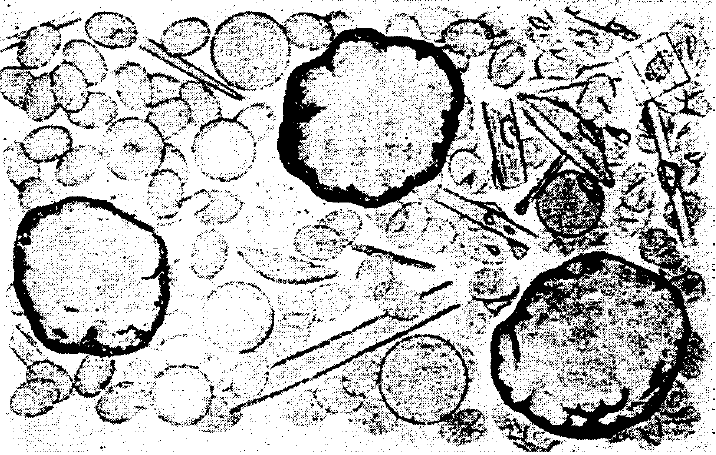
\includegraphics[width=0.7\textwidth]{introduction/chapter/figs/cells_extract.png}
  \caption{Diagrammatic representation of the crushing process: yeast ground with quartz sand and diatomite until the cells burst, the contents thereof emerging in the form of mucous lumps from the cell membrane. Illustration reproduced from \citet{buchner1907cell}}
  \label{fig.intro1}
\end{figure}


Endonucleases were another type of enzyme that revolutionised molecular biology. Endonucleases were discovered in the early 1960s \citep{arber1962host} by using one-step lysates from a $\lambda$ and/or P1 phage infected non-lysogenic \textit{Escherichia coli} K12 bacteria. Recognised as the "molecular scissors" protecting bacteria from bacteriophages, these restriction enzymes working in conjunction with methylases were capable of protecting the DNA of bacteria. Since the isolation of the first endonuclease from dialysed lysates of \textit{Escherichia coli} K, these started to be called restriction enzymes for their ability to "restrict" entrance of foreign genetic material, cutting it in as little as 10 to 30 seconds \citep{meselson1968dna}. Their specificity was later confirmed by \citet{kelly1970restriction} who described the 6 bp specific cleavage site of an endonuclease isolated from \textit{Haemophilus influenzae Rd} (Figure \ref{fig.intro2}). Enzyme later named as HindII by using the genus and species name of the host organism in a three-letter code, followed by the strain or type identification \citep{smith1973suggested}. The understanding of how restriction enzymes cut DNA, and how host DNA tries to protect itself became the basis of modern genetic engineering. 

\begin{figure}[!ht]
  \centering
  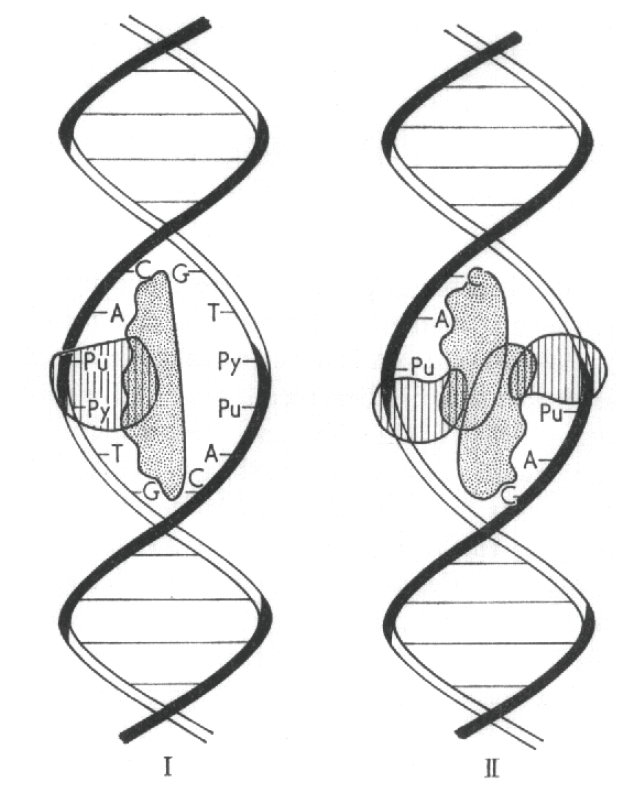
\includegraphics[width=0.7\textwidth]{introduction/chapter/figs/dnase.png}
  \caption{Recognition of a symmetrical nucleotide sequence by endonuclease R. Two possible models. Model I. A single enzyme molecule specifically binds to the base sequence GpTpPypPupApC.The active site of the enzyme (shaded area) catalyzes 5’-phosphoryl, 3’-hydroxyl cleavage of the phosphodiester bond between Py and Pu. The enzyme then detaches and attacks the other strand which (because of symmetry) contains the same base sequence. An even duplex break results. (Note: since endonuclease R is inactive on single-stranded DNA, it is necessary to assume in this model that the enzyme in some way “senses” the bihelical configuration of the substrate). 
  Model II. The enzyme is composed of two identical subunits (related by a g-fold rotational axis of symmetry) which bind to the sequence pPupApC on opposite strands of the DNA duplex. Each subunit is actually a dimer constructed from a “recognition” subunit (stippled) and a "nuclease" subunit (shaded). The recognition subunits bind to A and C, while the nuclease subunits bind to Pu. Hydrolysis of the phosphodiester bonds between Py and Pu by the nuclease subunits results in a duplex break. Illustration reproduced from \citet{kelly1970restriction}}
  \label{fig.intro2}
\end{figure}

Recombinant DNA molecules were created for the first time by the fusion of genetic material from more than one species \citep{jackson1972biochemical}. Here the DNA from two viruses, SV40 and $\lambda$, and the galactose operon of \textit{E. coli}  was cut creating “sticky ends” and the ends annealed and sealed with the addition of DNA polymerase and DNA ligase, forming one covalently closed-circular DNA molecule (Figure \ref{fig.intro3}). This was further confirmed by observing via gel electrophoresis, and comparing with previous SV40 viral genome observations performed by \citet{danna1971specific}, who created this now well-known visualization technique (Figure \ref{fig.intro4}), and gave a vital foundation for the later generation of genomic mapping.

\begin{figure}[!ht]
  \centering
  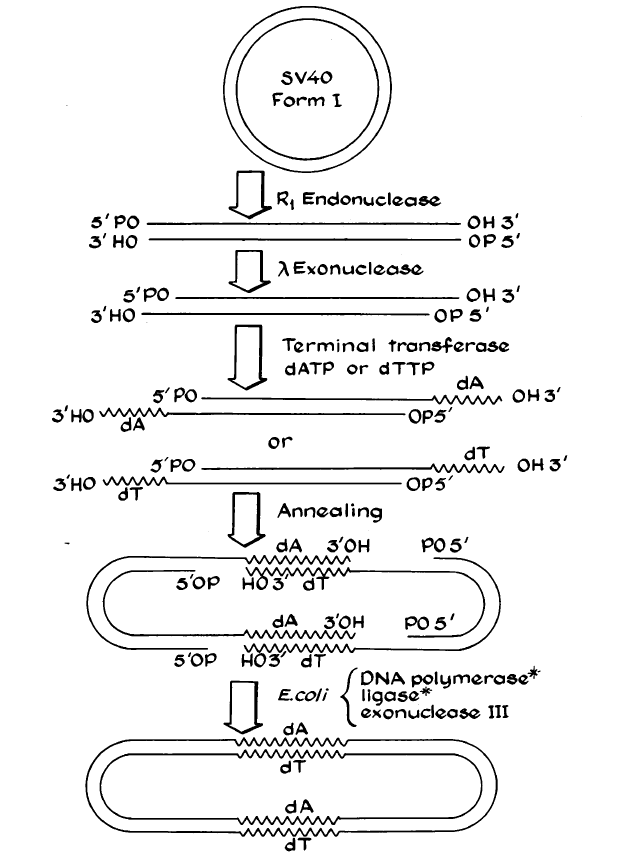
\includegraphics[width=0.7\textwidth]{introduction/chapter/figs/recombinant.png}
  \caption{General protocol for producing covalently closed
SV40 dimer circles from SV40(I) DNA. *The four deoxynucleoside triphosphates and NAD are also present for the DNA polymerase and ligase reactions, respectively. Illustration reproduced from \citet{jackson1972biochemical}}
  \label{fig.intro3}
\end{figure}

The introduction of recombinant DNA into living organisms was achieved by \citet{cohen1973construction}, proving that DNA can not only replicate naturally, despite being artificially introduced into another organism, but also can ligate in vivo. Since this work also proved that reassociated molecules carrying antibiotic resistance genes are capable of replication, can circularize and can be recovered as functional plasmids by appropriate selection, it establishes the principles of recombinant DNA technology and opens a new era of scientific discovery. 

A novel method for determining nucleotide sequences in DNA was described by \citet{sanger1977dna} making use of the 2',3'-dideoxy and arabinonucleoside analogues of the normal deoxynucleoside triphosphates, which act as specific chain-terminating inhibitors of DNA polymerase. Allowing to determine the sequence from 15 to around 200 nucleotides from the priming site with reasonable accuracy using a single primer \ref{fig.intro6}.

\begin{figure}[!ht]
  \centering
  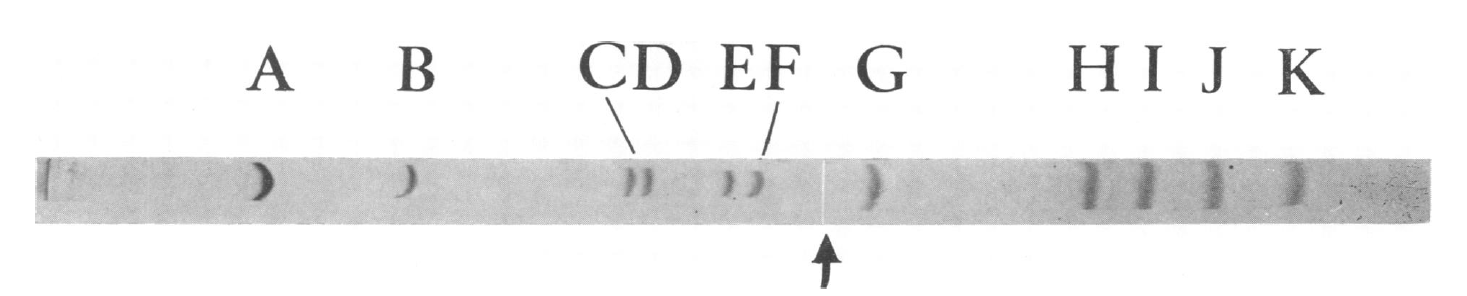
\includegraphics[width=0.7\textwidth]{introduction/chapter/figs/electrophoresis.png}
  \caption{Radioautographic analysis of SV40 DNA digested with \textit{H. influenzae} restriction endonuclease. 1 $\mu$g of SV40 [$^{14}$C]-DNA I (3 X 10$^4$ cpm/$\mu$g) was digested (see Fig. 2) for 6 hr in a volume of 55 $\mu$l; 0.0015 unit of enzyme was added at 0 time and at 1, 2, 3, 4, and 5 hr. 20 $\mu$l of sample was electrophoresed for 12.3 hr and the radioautogram was prepared as described in Methods \citep{danna1971specific}. The origin is at the left. The arrow below the radioautogram indicates a transverse cut made in the gel prior to slicing. Illustration reproduced from \citet{danna1971specific}}
  \label{fig.intro4}
\end{figure}

 As seen, molecular biology and genetic engineering have its genesis in a test tube looking for the origins of life in a liquid format; and cell extracts are present since their inception, hence, also in Synthetic Biology. The first \textit{in vitro} translation via the usage of cell-extracts \citep{miller1970visualization} demonstrated that RNA and protein synthesis can occur almost simultaneously in the cell, process that can be completely replicated in a test tube \ref{fig.intro7}. Thus, the usage of cell-free technology is not a new approach, and neither is Synthetic Biology. For instance, one of the first mentions of Synthetic Biology as a term can be traced back to \citet{leduc1912biologie}, who sought to synthesise life "by directing the physical forces which are its cause" and strongly stated that "It is in the physico-chemistry of liquids that an explanation of the phenomena of life is to be sought". 
The interconnection between liquids and life was a current of thought shared also by \citet{haldane1926mathematical} who proposed that the primordial sea served as a vast chemical laboratory powered by solar energy. Furthermore, \citet{oparin1924proiskhozhedenie} mentions that the first living beings found organic compounds, abiogenically formed, even highlighting that on the one hand, the synthesis of proteins requires the presence of nucleic acids while, on the other, the synthesis of nucleic acids requires the presence of proteins (enzymes).  By mixing inorganic constituents, nucleic acids and proteins, many authors looked for the ultramicroscopic particle endowed with catalytic and self-replicating properties of which the influences were able to permeate the entire cell, named at that time as genes \citep{muller1922variation}. Mixing of genes and other biomolecules would allow the synthesis of macronutrients, such as lactose achieved by Rohman (1919) by using extracts from mammary gland \citep{wasteneys1930enzymatic}. 



\begin{figure}[!ht]
  \centering
  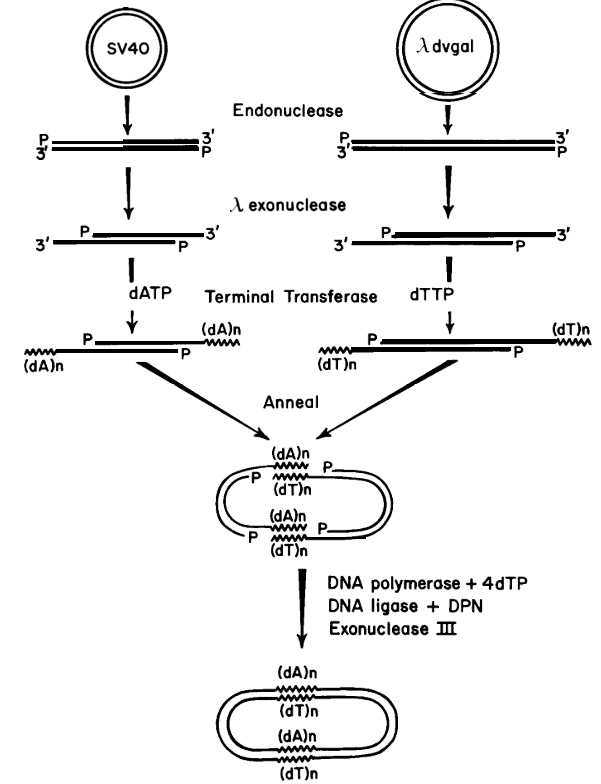
\includegraphics[width=0.7\textwidth]{introduction/chapter/figs/cohen.png}
  \caption{The construction of SV40-$\lambda\delta$ gal recombinant DNA. Illustration reproduced from \citet{berg1981dissections}}
  \label{fig.intro5}
\end{figure}

Looking for genes and the origin of life is that Teleonomy born reinstating the apparent purposefulness of structures and functions in living organisms, usually triggered by natural processes like natural selection. In 1961, after the “Cold Spring Harbor symposia on quantitative biology” \citet{monod1961general} tried to reconsider the problem of cellular regulation, summarising the discussions held and concluding that certain systems which appeared entirely different from one another are in fact submitted to similar, if not identical, controls that are in turn organised into different but also specific circuits. Basing themselves into Henri-Michaelis kinetics and Haldane equations they reintroduce mass action as one of the controlling factors in any enzyme-catalysed reaction, explaining that enzyme activity molecularly depends on their environment for their activation and inhibition (explaining competitiveness, allosteric reactions and feedbacks), molecular conversion (from zymogens to active enzymes and/or change in specificity), synthesis (associated to controlled compartments), stabilisation (connected to a wide variety of "circuits", endowed with any desired degree of stability), the gene expression that controls it (mentioning regulators, operators, operons, activators and transcriptional units) and the possible existence of an intermediate step between DNA and ribosomes, named messenger RNA, which existence was later confirmed by \citet{hurwitz1963role}. 


\begin{figure}[!ht]
  \centering
  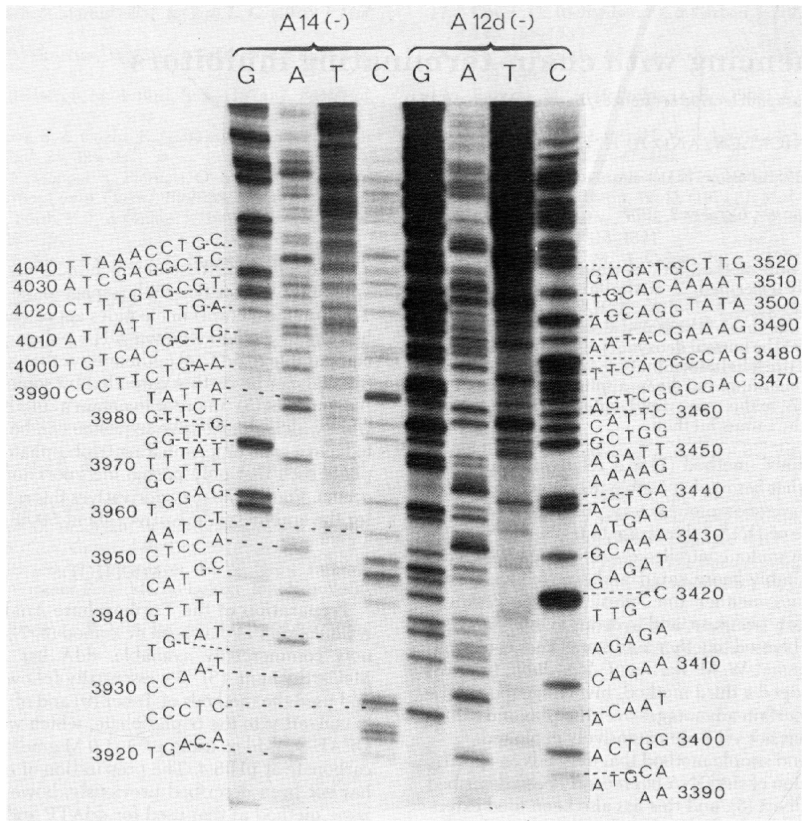
\includegraphics[width=0.7\textwidth]{introduction/chapter/figs/sanger.png}
  \caption{Autoradiograph of the acrylamide gel from the sequence determination using restriction fragments A12d and A14 as primers on the complementary strand of $\phi$X174 DNA. The inhibitor used were (left to right). The inhibitors used were (left to right) ddGTP, ddATP, ddTTP and araCTP. Electrophoresis was on a 12\% acrylamide gel at 40 mA for 14 hr. The top 10 cm of the gel is not shown. The DNA sequence is written from left to right and upwards beside the corresponding bands on the radioautograph. Illustration reproduced from \citet{sanger1977dna}}
  \label{fig.intro6}
\end{figure}

The rise of the “omics” era together with the perfectioning and widespread of complete-genome sequencing techniques led to what is currently known as Synthetic Biology \citep{cameron2014brief}, where the genetic knowledge is applied to create novel architectures going even further than what can be found in living organisms. On the start of the 21st century two synthetic genetic circuits were published, a toggle switch requiring external but transient induction instead of a sustained over time as occurs in living systems \citep{gardner2000construction} and a repressilator that uses decontextualised but naturally occurring genetic components to generate oscillatory transcriptional networks \citep{elowitz2000synthetic}.

Natural systems can be explained by studying simple synthetic circuits. For example, expression at single cell-level shows that noise plays an important role in bacteria during gene expression \citep{elowitz2002stochastic}; RNA circuits with engineered riboregulators showed the possibility to block recognition of the RBS using a \textit{cis}-repressed mRNA (crRNA) and further activation via a trans-activating RNA (taRNA) that hybridises with the crRNA, showing post-transcriptional control in both in vitro and in vivo \citep{isaacs2004engineered}; cell–cell communication and intracellular signal processing has also been explained  using synthetic multicellular consortia capable of pattern formation \citep{basu2005synthetic}; Novel discoveries in transcriptional regulation using genetic circuits allowed the generation of unnatural genetic networks \citep{alon2007network}.

Since site-specific recombination leaves short sequences in the final construct (recombination site), new cloning techniques were developed to have more accurate and efficient ways of genetic circuit generation.  Golden gate allows to create up to 256 different 4 nt overhangs using an alternative subcloning strategy that uses Type IIs restriction enzymes \citep{engler2008one}, which can cleave DNA outside of their recognition site and leave DNA overhangs consisting of any sequence allowing to clone with unique insert precision. Another assembly method that revolutionized the industry was Gibson assembly. By using a 5’ exonuclease, a DNA polymerase, and a DNA ligase this technic allows the assembly of synthetic and natural genes, genetic pathways and even entire genomes in an isothermal single reaction method \citep{gibson2009enzymatic}. 

With the advances in cloning strategies, synthetic circuits started becoming more advanced and complex. RNA devices able to execute higher-order cellular information processing operations from standard components were engineered as devices functioning as logic gates (AND, NOR, NAND, or OR gates) and signal filters, even exhibiting cooperativity \citep{win2008higher}. Multicellular biocomputing was achieved by using genetically encoded NOR gates via the generation of quorum sensing molecules by simple genetic circuits distributed in multiple cells, generating complex computation, such as XOR and EQUALS functions) in multicellular consortia \citep{tamsir2011robust}. 

Via the construction of single input–single output RNA devices, consisting of a sensor component, made of an RNA aptamer, an actuator component, made of a hammerhead ribozyme, and a transmitter component, made of a sequence that couples the sensor and actuator components, simple RNA devices that function as single-input Buffer and Inverter gates that convert a molecular input to increased and decreased gene expression output were created \citep{win2008higher}. More advances in RNA usage for genetical engineering was achieved by \cite{jinek2012programmable} revolutionising the industry. Here the system providing adaptive immunity against viruses and plasmids on bacteria and archaea was used to create a dual-RNA-guided DNA endonuclease. Clustered regularly interspaced short palindromic repeats (CRISPR) associated with the Cas endonuclease allows to cleave sequence-sepecific DNA generating an RNA programmable genome editing technic. 

\citet{paige2011rna} designed synthetic fluorescent RNA aptamers that mimic fluorescent proteins without the need for translation. The secondary structure of these aptamers presents a loop in which a fluorophore is trapped, conferring the same intramolecular immobilization that confers fluorescence in fluorescent proteins \citep{paige2011rna, strack2013superfolding}. The usage of RNA instead of proteins as output signal enhances the efficiency and response of synthetic circuits which added to recent advances in RNA technology broadens the possibility of their usage.

The expanded knowledge beyond the cell functionality created a path for the creation of Cell-free Synthetic Biology \citep{hodgman2012cell}. Cell-free expression systems are a powerful tool based in the early studies about expression originated in the 1960s-1970s with the added knowledge from current research. Cell-free systems are a powerful tool in applications where cell-based expression is too variable, slow, difficult to store or prohibitive due to legislation on the release of genetically modified organisms. 

\begin{figure}[!ht]
  \centering
  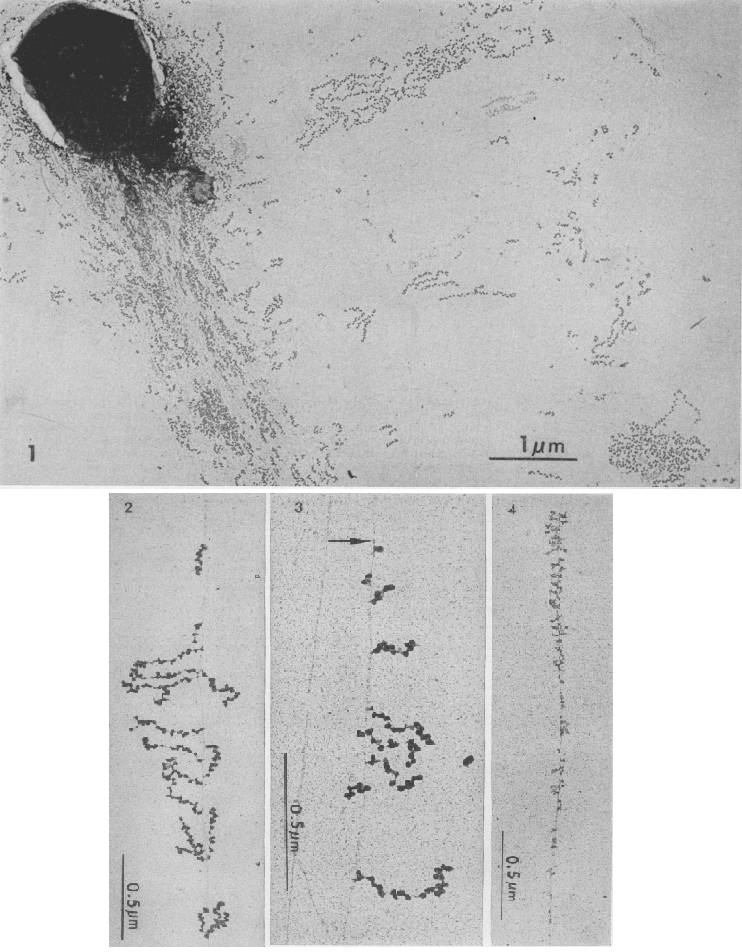
\includegraphics[width=0.7\textwidth]{introduction/chapter/figs/miller.png}
  \caption{Electron micrograph showing a portion of the extruded contents of an osmotically ruptured \textit{E. coli} cell. Fragile cells (2) were burst by rapid dilution (1:50) into distilled water adjusted to pH 9. The burst cells were immediately centrifuged (3200 rev/min at 19.3 cm radius for 3 to 5 minutes) through a O.1 M sucrose plus 10 percent formalin (pH 8.5) cushion onto carbon coated grids. The grids were rinsed in 0.4 percent Kodak Photo-flo, dried, and stained for 1 minute each in 1 percent phosphotungstic acid and 1 percent uranyl acetate, with both stains dissolved in 70 percent ethanol. The grids were then rinsed briefly in 95 percent ethanol, 100 percent ethanol, and isopentane and air-dried. Illustration reproduced from \citet{miller1970visualization}}
  \label{fig.intro7}
\end{figure}

This thesis tries solving diverse issues currently present in Synthetic Biology. Firstly, it starts by proposing an alternative approach to biological logic-gate creation, ParAlleL, which decomposes a large genetic circuit into a collection of small subcircuits, solved in parallel. Rather than having a single type of cell (or genetic material) doing the computation, here is used separate versions (subcircuits) each reacting to a different combination of inputs and generating the desired response by combination of each final output. This system allows the processing of up to 3 input bits, the pattern formation of a digital-like display and a Full adder and substractor.
Secondly, since the simplicity of cell-free systems can become a disadvantage when complex processes need to be performed or where genetic pathways from non-model organisms or obtained by metagenomic studies need to be expressed, here is also presented a novel cell-free system generated from the non-model bacteria \textit{Cupriavidus metallidurans} with heavy metal sensing capability for arsenic, mercury, cadmium, copper, zinc once coupled to RNA aptamers, and further discusses about Tx-only cell free systems. 
Finally, to reinforce the need of cell-free systems here is also explained the need for cell free systems generated from non-model  organisms by explaining how genetical engineering on subjects like \textit{Cupriavidus metallidurans} can trigger the generation of unintentional genomic changes hardening their usage in Synthetic Biology which is also later discussed in greater extension.
\renewcommand{\dir}{../chapter1/chapter/}
\chapter{ParAlleL: A Novel Population-Based Approach to Biological Logic Gates}

\section{Foreword}

This chapter refers to the work developed as a proof of concept for a parallel genetic circuit. Here multiple antibiotic resistance markers are transformed inside \textit{Escherichia coli} JM109 and used as a response to inputs of up to three bits. Each antibiotic represents either a binary zero or one notation. Once the subcircuit cells are mixed properly in a compartmentalised way, cells show binary consensus response in a death/alive format.

The work was published as a research article entitled “ParAlleL: A Novel Population-Based Approach to Biological Logic Gates” in the peer-reviewed journal Frontiers in Bioengineering and Biotechnology. Sections from 2.2 to 2.9 encompass the published manuscript including its Supplementary Information. Additional information, official links and repositories are mentioned within the chapter text. 

\section{Abstract}

In vivo logic gates have proven difficult to combine into larger devices. Our cell-based logic system, ParAlleL, decomposes a large circuit into a collection of small subcircuits working in parallel,
each subcircuit responding to a different combination of inputs. 
A final global output is then generated by a combination of the responses. Using ParAlleL, for the first time a completely functional 3-bit full adder and full subtractor were generated using 
\textit{Escherichia coli} cells, as well as a calculator-style display that shows a numeric result, 
from 0 to 7, when the proper 3 bit binary inputs are introduced into the system. 
ParAlleL demonstrates the use of a parallel approach for the design of cell-based logic gates that facilitates 
the generation and analysis of complex processes, without the need for complex genetic engineering.

\section{Introduction}

A major challenge in the field of synthetic biology is the construction of complex logic circuits that analyze variables as in electronics; where a single circuit accepts one or more binary inputs to generate one or more binary outputs. A cell-based logic network consists of engineered cells producing an output macromolecule only if the corresponding pattern of inputs is present. The mechanism of analysis is commonly based on the use of transcriptional regulators, transcription factors, polymerases, receptors, or recombinases \citep{brenner2018synthetic}. Some examples of genetic circuits mimicking computational behavior are toggle switches, oscillators, boolean logic gates, feedback controllers, and multiplexers. Although there are genetic circuits that simulate computational behavior, the complex engineering of their biological chassis is affected by gene expression noise, mutation, cell death, undefined, and changing extracellular environments and improper interactions with the cellular context \citep{andrianantoandro2006synthetic}. Furthermore, complex genetic engineering is necessary when multiple input variables are analyzed, limiting the processing capacity of the system.


Biological multiplexers analyze one or more signals over a common transmission line using interconnected transcription factors, recombinases, antisense RNA, or CRISPR-like technology \citep{nielsen2014multi,roquet2016synthetic,brenner2018synthetic}. However, complex genetic engineering is needed for wiring the basic computational units, becoming inefficient for moving beyond simple NOT or AND logic gates or for scaling to 3 bit logic circuits. The complexity of the genetic engineering required can be reduced by using distributed logic circuits, where the computation is distributed among several physically separated cellular consortia that each sense only one signal and respond by secreting a communication molecule \citep{regot2011distributed}. As a circuit responds to one signal, but not another, due to spatial distribution, a change in the state of the system can be triggered as response, making synthetic learning possible \citep{macia2017synthetic,shipman2017crispr}. Even though the consortium approach makes Boolean circuit design simpler, it still shows a slow response and considerable complexity since each cell needs to recognize, synthesize and secrete a wiring molecule \citep{macia2016implementation}.

Here we propose an alternative logic architecture, which decomposes a large circuit into a collection of small subcircuits acting in parallel (hereafter ParAlleL). Rather than having a single type of agent (such as a genetically engineered cell) doing the computation, ParAlleL has separate types of agent that each react to a different combination of inputs. A final output is then generated by combination of the responses, making all kinds of binary operation possible. As an example, here we show the implementation of this concept using cells resistant to different combinations of antibiotics, with the response indicated by growth. This is used to demonstrate a completely functional 3 bit full adder and full subtractor, as well as a calculator-style display that shows digits from 0 to 7 based on three binary input bits.

\section{Methodology}

\subsection{Reagents and Stock Solution Preparations}

Antibiotic stock solutions were prepared as follows: 100 mg/ml carbenicilin disodium salt (Sigma-Aldrich \#C1389), 50 mg/ml kanamycin sulfate (PanReac Applichem \#A1493), 20 mg/ml chloramphenicol (Acros Organics \#22792), 10 mg/ml tetracycline hydrochloryde (Duchefa Biochemie \#T0150), 10 mg/ml gentamicin sulfate (Melford \#G0124), and 50 mg/ml spectinomycin.HCl (LKT Labs \#S6018). Developing solution contained 0.1 \%w/v bromothymol blue (Sigma-Aldrich \#114421) and 400 mM Trizma base pH7.5 (Sigma-Aldrich \#T1503).

\subsection{Generation of Subcircuit Cells}

\textit{E. coli} JM109 was transformed with 200–300 pg of plasmid pSB4A5 (AmpR) or pSB4C5 (ChlR) (Registry of Standard Biological Parts) and selected on 100 $\mu$g/ml carbenicilin (Am) or 20 $\mu$g/ml chloramphenicol (Ch), respectively. Cells carrying the first bit plasmid were made chemically competent \citep{chung1989one} and transformed with 200–300 pg of the 2nd bit plasmid, pSB1T3 (TetR) or pSB1K3 (KanR) (Registry of Standard Biological Parts). Selection was performed with the first antibiotic (Am or Ch) and the addition of 10 $\mu$g/ml Tetracycline (Tc) or 50 $\mu$g/ml kanamycin (Km), obtaining the two-bit combinations Km/Am (KA), Tc/Am (TA), Km/Ch (KC), and Tc/Ch (TC). This set of strains is sufficient to implement all two-bit binary operations.

The third bit layer was generated by transforming these four strains with pSEVA631 (GenR) \citep{silva2012standard} (GenBank JX560348) or pMO9075 (SpmR) \citep{keller2011methods}. Resulting strains were selected on the 2-bit antibiotic combinations plus 10 $\mu$g/ml gentamicin (Gm) or 50 $\mu$g/ml spectinomycin (Sm). This gave 8 strains, designated ATG (Am/Tc/Gm), AKG (Am/Km/Gm), ATS (Am/Tc/Sm), AKS (Am/Km/Sm), CTG (Ch/Tc/Gm), CTS (Ch/Tc/Sm), CKG (Ch/Km/Gm), CKS (Ch/Km/Sm) based on their resistance markers. This set of strains is sufficient to implement all three-bit binary operations. Plasmid specifications are listed in Figure \ref{fig.parallel4}, Tables \ref{table:11}, \ref{table:12}, with further information about these antibiotics in Table \ref{table:13}. Plasmid sequences are available in different formats at https://doi.org/10.7488/ds/2497.

\subsection{Three-Bit Logic Operations}

Tests were performed in 96-well microplates by inoculating cells (1:100) in LB broth (100 $\mu$L) supplemented with 1\%w/v D(+)-glucose (Fisher Chemical \#G0500). Plates were incubated for 18 h at 37$^{\circ}$C without shaking and then developed by addition of the developing solution (0.1\%w/v bromothymol blue in 400 mM Tris, pH 7.5) in a ratio 1:20. Images were obtained using a Kodak ESPC315 Flatbed scanner. Design of the calculator-like display, full adder, and subtractor are shown in Figures \ref{fig.parallel2}, \ref{fig.parallel3}. Raw figures were deposited at https://doi.org/10.7488/ds/2497.

\section{Results}

In the distributed logic system of ParAlleL each input bit has two forms, ZERO and ONE, each of which is essential to certain output agents and inhibitory to others. Thus each agent reacts only to a certain combination of input bits, allowing generation of any arbitrary pattern of outputs for any pattern of inputs. In the implementation shown here, each input bit comes in two forms, each being an antibiotic lethal to sensitive strains. In this case, bit A is represented by ampicillin for zero, chloramphenicol for one, bit B by kanamycin for zero, tetracycline for one, and bit C by gentamicin for zero, spectinomycin for one. Thus, four strains are needed to implement any operation with two input bits, and eight strains for three input bits. In contrast to other cell-based logic schemes, only very minimal genetic engineering is required, essentially transformation with 3 different antibiotic resistance markers.

Cells show a global response concordant with the behavior expected for a 1 bit, 2 bit, or 3 bit system (Figure \ref{fig.parallel1}). For instance, when the input 101 (chloramphenicol, tetracycline and spectinomycin) is added to the system growth is only observed in the corresponding CTS cells, which carry the proper resistance markers. The response time of the system is around 12 h (Figure \ref{fig.parallel5}) but plates were developed at 18 h to avoid false negatives or positives.

\begin{figure}[h]
  \centering
  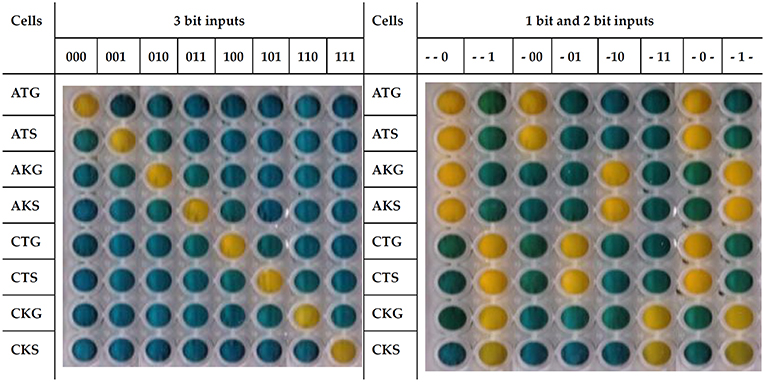
\includegraphics[width=0.7\textwidth]{chapter1/chapter/figs/fbioe-07-00046-g001.jpg}
  \caption{ParAlleL responding to 1 bit, 2 bit, and 3 bit inputs. ParAlleL subcircuit cells were spatially distributed in different wells (vertically) and exposed to specified 1 bit, 2 bit, or 3 bit inputs (top of each column). Cells were inoculated (1:100) in LB supplemented with 1\% w/v glucose. After 18 h of incubation at 37$^\circ$C, plates were developed by addition of 0.05 volumes of the developing solution.}
  \label{fig.parallel1}
\end{figure}

In order to further test the ParAlleL system, a digital calculator-like display was designed (Figure \ref{fig.parallel2}A). In this case, multiple subcircuit cells are mixed in one well and the global response displays a number from 0 to 7 when the proper binary input is applied. Numbers represent the total eight possible values encoded within 3-bit binary inputs.

\begin{figure}[htbp]
  \centering
  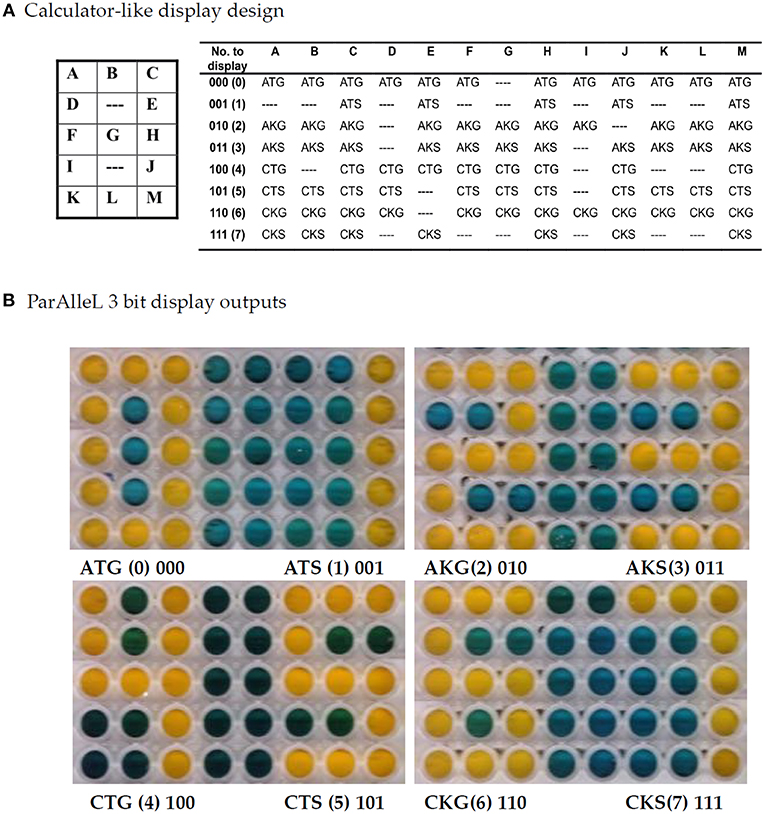
\includegraphics[width=0.7\textwidth]{\dir figs/fbioe-07-00046-g002.jpg}
  \caption{Digital calculator-like display using 3 bit ParAlleL. Figure shows all numerals from zero to seven based on the 8 binary inputs provided. (A) Subcircuit cells were mixed and distributed in a 3 × 5 matrix and inoculated (1:100) in LB supplemented with 1\%w/v glucose. Plate was developed after 18 h of incubation, by addition of 0.05 volumes of developing solution. (B) Output number results obtained by addition of each 3 bit antibiotic combination.}
  \label{fig.parallel2}
\end{figure}

Input configuration versatility was proven by representing bit A in this case by gentamicin for zero, spectinomycin for one, bit B by kanamycin for zero, tetracycline for one, and bit C by ampicillin for zero, chloramphenicol for one. For instance, once input 110 represented by Ch/Km/Gm is added in the system, the number 6 is displayed (Figure \ref{fig.parallel2}).

Finally, a full adder and a full subtractor were designed. A full-adder adds three binary inputs, often denoted as A, B, and C$_{in}$, generating a Sum result (S) and a Carry-out (C$_{out}$). A full subtractor, on the other hand, has a minuend (X), a subtrahend (Y) and an additional Borrow-in (B$_{in}$) as inputs. The subtraction operation produces a difference (D) and a Borrow (B$_{out}$) (Figure \ref{fig.parallel3}).
\begin{figure}[htbp]
  \centering
  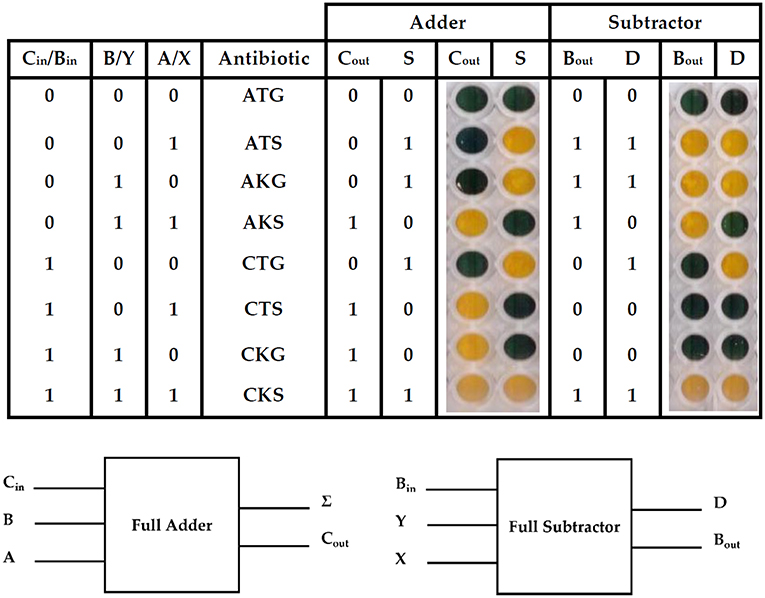
\includegraphics[width=0.7\textwidth]{\dir figs/fbioe-07-00046-g003.jpg}
  \caption{Full adder and subtractor using the 3 bit ParAlleL system. The figure shows results of addition and subtraction using the ParAlleL for 3 bit system. Cells were mixed and inoculated (1:100) in LB supplemented with 1\%w/v glucose. After 18 hours of incubation, the plate was developed by addition of the 0.05 volumes of developing solution.}
  \label{fig.parallel3}
\end{figure}

In order to generate the full adder and subtractor, multiple subcircuit cells were mixed and distributed in two different wells (Figure \ref{fig.parallel3}). One well represents the solution (S) or difference (D) and a second one the carry (C$_{out}$) or borrow (B$_{out}$), for the adder and subtractor, respectively (Figure \ref{fig.parallel3}). A yellow color represents growth and a positive output 1, a blue color represents no growth and a binary 0 output instead.

\section{Conclusions/Discussion}

Subcircuits that solve complex calculations in parallel have been extensively used for computation in order to reduce the total computation time. Translating this approach to biological systems would allow us to analyze complex processes, currently difficult in synthetic biology, as multiple simple sub-circuits.

In our proof of concept, we present a biological information processing system, ParAlleL, capable of exploiting the parallelism in mixed bacterial cultures. ParAlleL decomposes the analysis of 2 and 3 bit complex inputs, into 4 and 8 sub circuits, respectively (Figure \ref{fig.parallel1}). Each sub-circuit corresponds to a different \textit{E. coli} strain carrying a different combination of antibiotic resistance markers (Table \ref{table:11}). As an example, in the 3 bit system the input 000 is represented by the antibiotics ampicillin, tetracycline and gentamicin (Figure \ref{fig.parallel1}). When this input is entered into the system, all cells that are not encoded for responding to 000 will die, but cells carrying the proper plasmid combination, pSB4A5, pSB1T3, and pSEVA621 will not (Figures \ref{fig.parallel1}, \ref{fig.parallel2}), therefore, a live/dead response (output) is achieved in all sub circuits, the output of each well being one (growth) or zero (failure to grow) (Figure \ref{fig.parallel2} and Figure \ref{fig.parallel4}).

\begin{figure}[htbp]
  \centering
  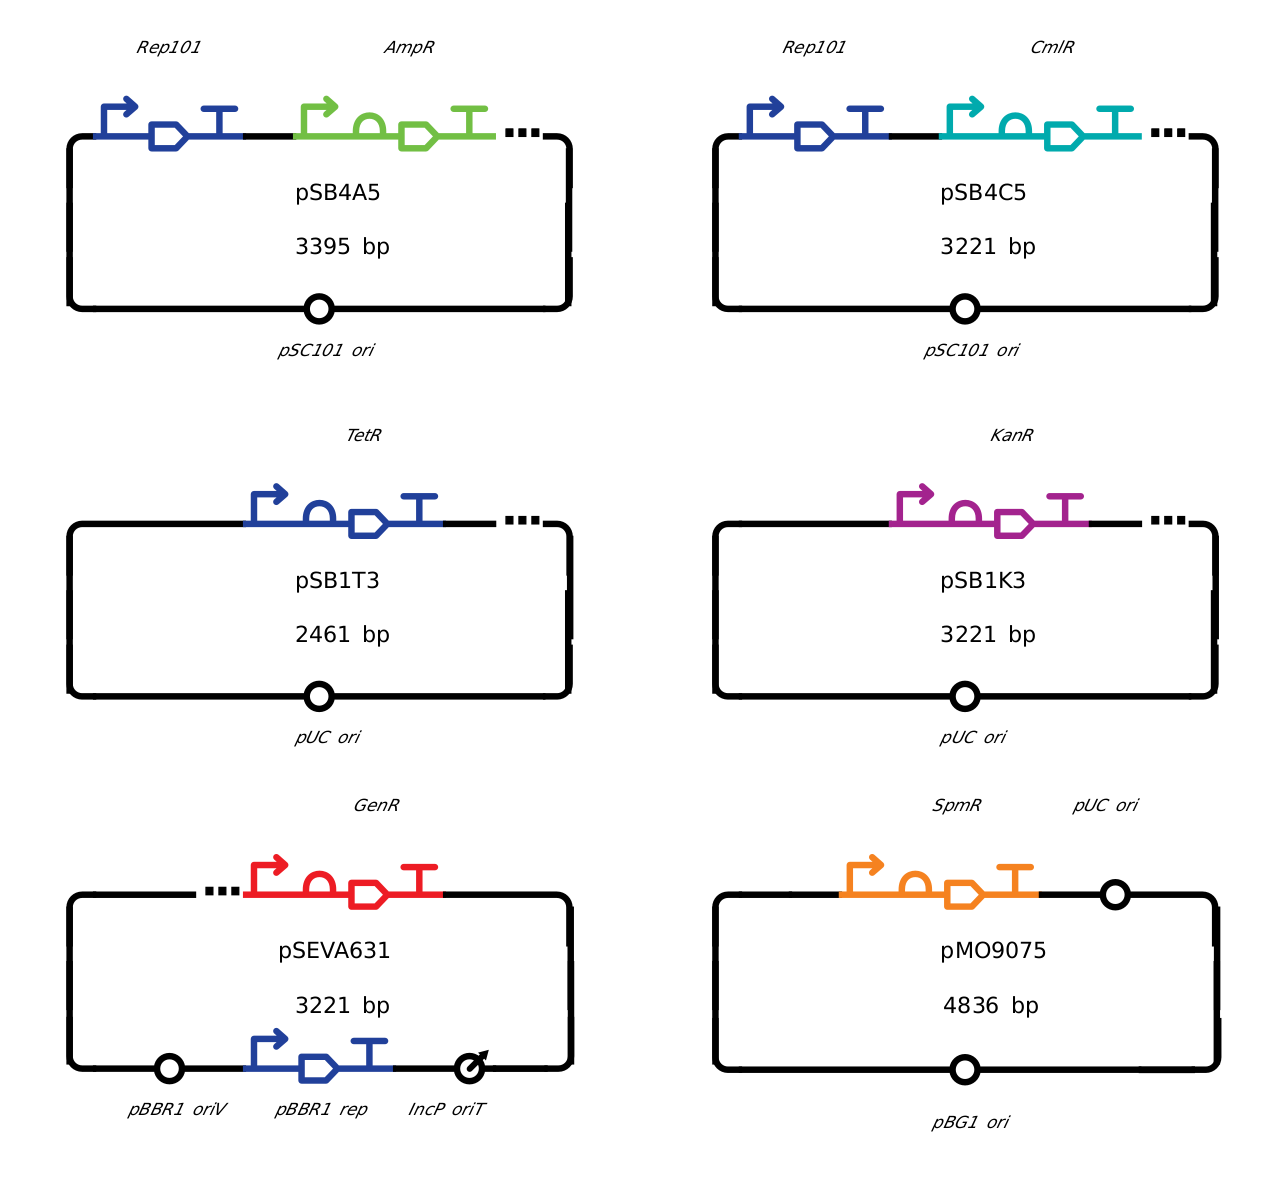
\includegraphics[width=0.7\textwidth]{\dir figs/plasmids.png}
  \caption{Plasmids carried by subcircuit cells. Plasmids carrying antibiotic resistances for Ampicillin (pSB4A5); Chloramphenicol (pSB4C5); Tetracycline (pSB1T3); Kanamycin (pSB1K3); Gentamicin (pSEVA631) and Spectinomycin (pMO9075) represented in SBOL format. Plasmid sequences available at https://doi.org/10.7488/ds/2497.}
  \label{fig.parallel4}
\end{figure}

ParAlleL uses cellular consortia instead of a single type of cell. A similar approach has been developed by \citet{macia2016implementation} using eukaryotic cells, and even showing the possibility of generating transient memory. However, that approach requires a sophisticated design as it relies on a secreted intermediate molecule (hormone-like) that must be kept at the right production level, and that should be previously activated by X (Repressor) and Y (SsrA-tagged protein) degradation. Furthermore, since the output of the circuit is distributed among different consortia, the concentration of the secreted molecule can differ according to the number of cells simultaneously producing it. This kind of multicellular approach and others based on single cells require sophisticated wiring design \citep{silva2008mining,siuti2013synthetic,macia2016implementation,macia2017synthetic}. By contrast, ParAlleL requires very minimal genetic modification and little tuning to obtain reliable outputs (Figures \ref{fig.parallel2}, \ref{fig.parallel3}).

\begin{figure}[htbp]
  \centering
  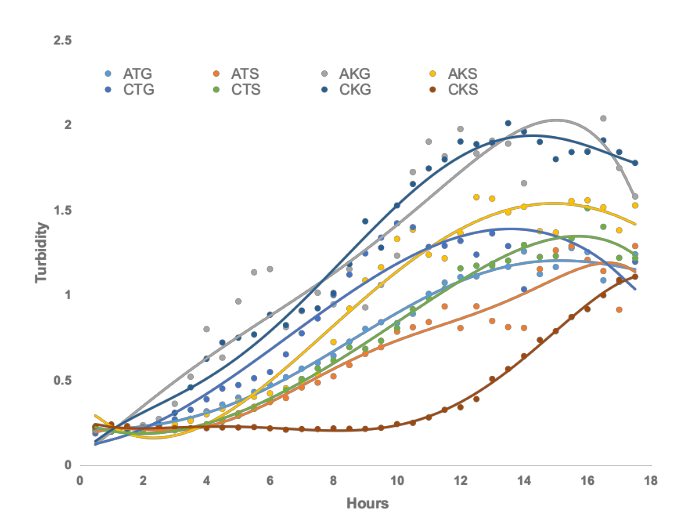
\includegraphics[width=0.7\textwidth]{\dir figs/growth.png}
  \caption{ParAlleL subcircuit cell growth curves. Growth curves of the 3-bit subcircuit cells in LB + 0.1\% glucose with their respective antibiotic combinations. A: Carbenicilin (100 $\mu$g/mL), C: Chloramphenicol (20 $\mu$g/mL) T: Tetracycline (10 $\mu$g/mL), K: Kanamycin (50 $\mu$g/mL), G: Gentamicin (10 $\mu$g/mL). S: Spectinomycin (50 $\mu$g/mL). Overnight culture (0.01 volume) was used as inoculum.}
  \label{fig.parallel5}
\end{figure}


The implementation of ParAlleL presented here is simple, but its further development to useful applications presents a number of challenges. Firstly, expansion to 4 bits and beyond would require further well-behaved and non-cross-reacting antibiotic resistance markers, and would probably lead to even greater disparities in growth rate than those observed in the three-bit system (Figure \ref{fig.parallel5}). This could be addressed, and the flexibility and usefulness of the system increased, by moving away from direct use of antibiotics to a system using tightly controlled inducible promoters, each controlling a lethal “death gene,” such as \textit{ccdB}, with either the presence or absence of the inducer leading to lethality. In this way the system could be made to respond to different combinations of useful inputs, for example in the construction of multiplexed biosensors.

However, to achieve the full potential of ParAlleL, it will be necessary to generate layered systems in which the output from one layer serves as input to another layer. This might be accomplished via quorum sensing, but the implementation would be rather complex and limited. A more attractive option is to transfer the same concept, using a set of agents which each responds to a single combination of inputs, to an alternative system. For example, the concept could be implemented in a cell-free system, in which inputs may be present as small molecules interacting with transcription factors, or as DNA or RNA oligonucleotides. Outputs from the first layer, in the form of DNA or RNA molecules generated by DNA replication (e.g., PCR) or transcription, could then serve as inputs to a second layer. For example, in a PCR-based approach, one of a set of templates would be amplified based on which primer oligonucleotides were added; the output PCR product could then be processed to generate another set of oligonucleotides, or used directly to initiate priming on a second set of templates via formation of three-way junctions. Alternatively, in a transcription-based system, output RNAs from a first layer computation could act as guide RNAs directing binding of CRISPR-based transcription factors to further templates to generate a new set of guide RNAs, eventually leading to production of an output RNA such as a mRNA leading to translation of a visually detectable signal.

Another interesting aspect of ParAlleL is that, since the final output is the result of a population-based calculation, these systems may show a level of “Byzantine fault tolerance,” allowing reliable outcomes even in the face of levels of noise which are unavoidable in biological systems. This would represent a new level of robustness in biological computation systems.

\section{Data Availability}
All datasets generated for this study are included in the manuscript and/or the supplementary files. More Data is available at https://doi.org/10.7488/ds/2497

\section{Acknowledgments}

The authors acknowledge the valuable assistance of Dr. Louise Horsfall for supplying the pMO9075 plasmid and Dr. Aitor De las Heras for supplying the pSEVA631 plasmid. A pre-print version of the manuscript has been published on bioRxiv (Millacura et al., 2018).
\section{Supplementary Material}

The Supplementary Material for this article can be found online at: https://www.frontiersin.org/articles/10.3389/fbioe.2019.00046/full
\#supplementary-material

\begin{table}[htb]
%\captionsetup{labelformat=empty}
\caption{Plasmids used for generating ParAlleLsubcircuit strains.\\}
\label{table:11}%
{%\hspace*{-5cm}
\begin{tabular*}{\columnwidth}{@{}lllll@{}}
\hline
\textbf{Plasmid} & \textbf{Antibiotic} & \textbf{ORI} & \textbf{PCN$^*$}  & \textbf{Reference}\\
\hline
pSB4A5 & AmpR & pSC101 & 5 & $^{**}$Part:pSB4A5\\
pSB4C5 & CmlR & pSC101 & 5 & $^{**}$Part:pSB4C5\\
pSB1T3 & TetR & pMB1(der) & 100-300 & $^{**}$Part:pSB1T3\\
pSB1K3 & KanR & pMB1(der) & 100-300 & $^{**}$Part:pSB1K3\\
pSEVA631 & GenR & pBBR1 & medium & $^{***}$JX560348\\
pMO9075 & SpmR & pBG1 & low & \cite{keller2011methods}\\

\\
\hline
\hline
\end{tabular*}
}
\\
{
\footnotesize{$^*$PCN: Plasmid Copy Number}\\
\footnotesize{$^{**}$https://parts.igem.org/}\\
\footnotesize{$^{***}$https://www.ncbi.nlm.nih.gov/nuccore/}
}
\end{table}




\begin{sidewaystable}[ht]
%\captionsetup{labelformat=empty}
\caption{Antibiotics and resistance cassettes used on ParAlleL.\\}
\label{table:12}%
{%\hspace*{-5cm}
\begin{tabular*}{\columnwidth}{@{}lllll@{}}
\hline
\textbf{Antibiotic} & \textbf{Class} & \textbf{Mode of action} & \textbf{Resistance}   \\
 & &  & 
\\
\hline
Ampicillin & $\beta$-lactam & Bactericidal; Inhibits  cell  wall synthesis & $\beta$-lactamase (\textit{bla}) gene \\
Kanamycin  & Aminoglycoside & Bactericidal; Binds 30S ribosomal subunit;  & Neomycin phospho-\\
  &  & causes mistranslation & transferase II   \\
Chloramphenicol & Chloramphenicol & Bacteriostatic;    Binds    50S ribosomal subunit; & Chloramphenicol\\
 &  & inhibits peptidyl translocation & acetyl transferase \\
Tetracycline  & Tetracycline & Bacteriostatic;    Binds    16S ribosomal subunit; & Tetracycline efflux \\
  &  & inhibits protein synthesis (elongation step)  & protein  \\
Gentamicin & Aminoglycoside & Irreversibly binding the 30S subunit of the & Gentamicin-3-N-acetyl-\\
 &  & bacterial ribosome &  transferase \\
Spectinomycin & Aminocyclitol & It binds to the 30S and interrupts protein & Spectinomycin adenyl-\\
 &  & synthesis  affecting  16S rRNA & transferase \\
\\
\hline
\hline
\end{tabular*}
}
\\
{
%\footnotesize{}
}
\end{sidewaystable}


\begin{table}[ht]
%\captionsetup{labelformat=empty}
\caption{Plasmid incompatibility groups.\\}
\label{table:13}%
{%\hspace*{-5cm}
\begin{tabular*}{\columnwidth}{@{}lllll@{}}
\hline
\textbf{Incompatibility group} & \textbf{Regulation} & \textbf{Comment} \\
\hline
pBR322/ColE1/pMB1 & Inhibitor-target RNAI & Control processing of \\
& &  pre-RNAII into prime \\
IncFII, pT181 & RNA & Affecting synthesis of\\
 &  &  RepA protein \\
R6K$^*$ & Iteron binding & Sequestering of RepA \\
Rts1, P15A*, RK2 &  & protein\\
\\
\hline
\hline
\end{tabular*}
}
\\
{
%\footnotesize{}
}
\end{table}






\renewcommand{\dir}{../chapter2/chapter/}
\chapter{TXO: Transcription-Only genetic circuits as a novel cell-free approach for Synthetic Biology}

\section{Foreword}

In order to avoid using the cell-based approach, genetic circuits were prepared as cell-free systems using extracts from the non-model bacteria \textit{Cupriavidus metallidurans}. Cells were lysed using a non-ionic method allowing us to recover functional transcriptional regulators. Diverse heavy metals were detected by a mix of cell extract and small synthetic constructs carrying inducible promoters. Fluorescent RNA aptamers were used as output signal for the system, accelerating the observed response to a few minutes.

This work is currently under review as a research article entitled “TXO: Transcription-Only genetic circuits as a novel cell-free approach for Synthetic Biology” in the peer-reviewed journal NAR Synthetic Biology. Sections from 3.2 to 3.9 show the manuscript to be published including its Supplementary Information. Additional information, official links and repositories are mentioned within the chapter text. 

\section{Abstract }

While synthetic biology represents a promising approach to solve real-world problems, the use of genetically modified organisms is a cause of legal and environmental concerns. Cell-free systems have emerged as a possible solution but much work is needed to optimize their functionality and simplify their usage for Synthetic Biology. Here we present TXO, transcription-only genetic circuits, independent of translation or post-translation maturation. RNA aptamers are used as reaction output allowing the generation of fast, reliable and simple-to-design transcriptional units. TXO cell-free reactions and their possible applications are a promising new tool for fast and simple bench-to-market genetic circuit and biosensor applications.


\section{Introduction}

Cells, including microbial, plant and mammalian cells, have been long engineered for responding to a plethora of environmental factors, benefiting from their intrinsic ability to process the entire cycle from the recognition of a specific target, to analysis of the information, and generation of an output signal \citep{khalil2010synthetic}. However, cell-based systems present also unavoidable disadvantages during their usage, including the risk of releasing genetically modified organisms (GMOs) into the environment, accumulation of mutations and genetic instability, uncontrollable side-reactions within the cell, and issues with viability maintenance during long-term storage \citep{bousse1996whole,gupta2019cell,kaur2015advances, yagi2007applications}.
In order to solve these issues, cell-free systems (CFS), also known as transcription-translation (TX-TL) systems, have emerged as a promising alternative. CFS not only inherit most of the benefits from cell-based systems, but also avoid major challenges that they face. Typically, CFS are based on non-living cell-extracts or reconstituted systems that by not presenting a living prospect solve problems related to biosafety, cross-reactivity and long-term functionality maintenance. CFS are rather robust to factors that pose cellular stress, including sensitivity to toxic pollutants and to the typical “overload problem” observed when foreign “genetic circuits” are introduced into the cell \citep{borkowski2016overloaded}.
TX-TL systems share with cells a problem hindering their usage in real-time detection. Response time in TX-TL systems may need a long time for transcription, translation and post-translational maturation to occur, in order to finally produce a detectable signal. For instance, Pardee and colleagues \citep{pardee2016rapid} developed a cell-free paper toehold-switch sensor for detection of the Zika virus that takes hours for the final visual results to come out \citep{borkowski2016overloaded}. Paper-based cell-free sensors that detected heavy metals and gamma-hydroxybutyrate by expressing sfGFP needed at least one hour for producing a measurable response \citep{grawe2019paper}. Considering the need for in-situ field analysis, an improvement of cell-free systems response time is necessary \citep{ejeian2018biosensors,justino2017recent}.
Since CFS are open and easily modifiable systems \citep{niederholtmeyer2013implementation}, time-consuming translation and post-translational modification can be removed, allowing novel approaches with faster signal generation. Alternative output signals independent of translation and post-translational modification can provide the system with a simpler composition, lower resource requirements and, most importantly, a shorter response time. Here, we introduce a transcription-only (TXO) cell-free system using RNA aptamers as output signals rather than translated proteins.
Fluorescent RNA aptamers are short ribonucleotide sequences that upon binding a specific compound, enhance (amplify) or dequench its fluorescence. RNA aptamers, such as Spinach \citep{paige2011rna}, iSpinach \citep{autour2016ispinach} and Broccoli \citep{filonov2014broccoli} have shown excellent properties for generating bright and stable fluorescence. In the past few years, RNA aptamers have been widely applied in live-cell imaging \citep{neubacher2019rna} and biosensing \citep{cho2009applications}. However, these previously reported aptamer-based sensors acted as both sensing elements (binding to target molecules) and signal generator at the same time \citep{dehghani2018aptamer,razmi2018recent}, requiring aptamers specifically designed for each target. 
In TXO systems the functions for input detection (sensing), processing (analysis) and output generation (reporting) are decoupled, creating modular systems where aptamers can be used as universal signal generators. To exemplify the versatility of such system, here we used a simple cell-free extract from the microorganism \textit{Cupriavidus metallidurans} CH34, which carries most of the necessary heavy-metal (e.g., Hg$^+$, Pb$^{2+}$, Cu$^{2+}$, Zn$^{2+}$, Ni$^{2+}$, among others) responsive transcription factors and the RNA polymerase which they control \citep{monchy2007plasmids}. Since all necessary transcription factors are provided directly by the cell-free extract only the synthetic transcription unit must be changed to detect these different metal ions. Combining of the easy to design TXO system, with the high sensitivity of the sensing elements and the fast output signal generation provided by RNA aptamers, TXO is a promising tool for accelerating bench-to-market Synthetic Biology, most specifically where in-situ, simple to design and rapid applications are needed.


\section{Methodology}

\subsection*{Reagents and culture conditions}
Fluorophores DFHBI (Tocris \#5609), DFHO (Tocris \#6434), DMABI and 2-HBI (provided by Dr. Jaffrey’s laboratory at Cornell University) were dissolved in DMSO (Fisher Scientific \#BP231) to prepare 2 mM stock solutions (for further information see Table \ref{table:32}). Our optimised transcription/detection buffer (OTDB) was prepared as a 10X stock as follows: Tris base 400 mM pH 7.5 adjusted with HCl (Sigma-Aldrich, \#T1503); MgCl$_2$·6(H$_2$O) 60 mM (Sigma-Aldrich, \#M2670); DTT 100 mM (Melford, \#MB1015) and Spermidine 20 mM (Alfa Aesar, \#A19096.03). Metal-ion solutions were prepared from soluble salts of analytical grade: CuSO$_4$·5H$_2$O (Sigma-Aldrich \#C8027), Arsenite NaAsO$_2$ (Sigma-Aldrich \#202673), Pb(NO$_3$)$_2$ (Sigma-Aldrich \#228621), HgCl$_2$ (Sigma-Aldrich \#215465), ZnCl$_2$ (Sigma Aldrich \#229997) and NiCl$_2$·6H$_2$O (Fisher Scientific \#AC27051) in double-deionised water and filter-sterilised before use.


\subsection*{Strains and cell-free extract preparation}

\textit{C. metallidurans} CH34 cells were cultivated on a Tris-buffered mineral medium (MM284) \citep{mergeay1985alcaligenes} supplemented with succinate 0.4 \%w/v, at 30$^{\circ}$C with constant shaking at 180 RPM. Escherichia coli JM109 cells were grown on Luria Broth (LB) at 37$^{\circ}$C. For cell-extract preparation, cells were collected at middle exponential phase (OD 0.6-0.8) by centrifugation at 3,900 × g and 4$^{\circ}$C for 10 min. Cells were resuspended in one tenth of the centrifuged volume in a non-ionic lysis buffer, which contains Triton X-100 0.1\%v/v (Sigma-Aldrich \#T9284), Tris base (40 mM) adjusted to pH 7.5 with HCl and lysozyme 50 mg/mL (Sigma-Aldrich \#L6876) for 30 min at 4$^{\circ}$C. The lysed extract was centrifuged at 12,000 × \textit{g}, 4$^{\circ}$C for 20 min and the supernatant was immediately used or saved at -80$^{\circ}$C for later use.

\subsection*{Construction of RNA aptamers}

Aptamer sequences (see Table \ref{table:3.1}) protected within the F30 scaffold (upper and lower sections) were synthesised as 120 bp oligonucleotide sequences (Sigma-Aldrich), and then extended using the 5 bp shared on the 3’ of each oligonucleotide for the annealing (see Figure \ref{NAR-fig1} and Table \ref{table:331}) A PCR reaction adding a T7 promoter/terminator pair on each aptamer (see Table \ref{table:3.1}) was carried out using Q5 High-Fidelity DNA Polymerase (New England Biolabs Inc.(NEB) \#M0491) and the following protocol: 95$^{\circ}$C for 5 min (1 cycle), 95$^{\circ}$C for 20 s, 54$^{\circ}$C for 10s and 72$^{\circ}$C for 20 s (35 cycles), with a final elongation at 72$^{\circ}$C for 5 min. Amplification was analysed in a 1.5 \% (w/v) agarose gel and purified from the PCR reaction using the QIAquick PCR Purification Kit (Qiagen, \#28104), and subsequently cloned in to the pMini-T plasmid using the PCR Cloning Kit (NEB \#E1202). Plasmids were extracted from \textit{E. coli} JM109 transformed cells using the QIAprep Spin Miniprep Kit (Qiagen) and sequence verified by Sanger sequencing using the BigDye Terminator v3.1 Cycle Sequencing Kit (Thermo Fisher Scientific) and an Applied Biosystems 3730XL DNA Analyzer (Edinburgh Genomics). 

\begin{figure*}[ht]
\begin{center}
\hspace*{0cm}
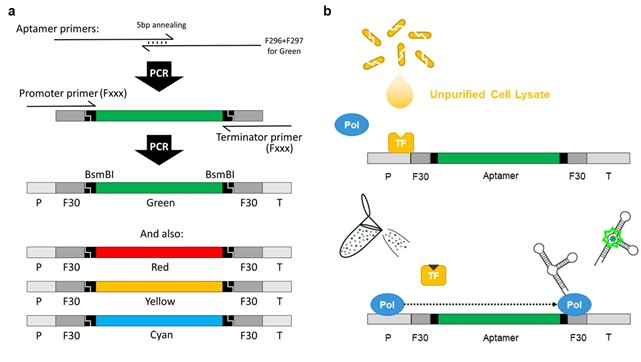
\includegraphics[height=220px]{./chapter2/chapter/figs/Imagen1.jpg}
\end{center}
\caption{Schematic diagrams of TXO cell free system with minimal requirements. \textbf{(a)} Sequence and production process of diverse RNA aptamers via PCR, showing addition of BsmBI sites for further Golden Gate manipulation. \textbf{(b)} In a TXO system there are minimal requirements such as an inducer, moderator/repressor, RNA polymerase and a final RNA output herewith represented as a fluorescent aptamer.}
\label{NAR-fig1}
\end{figure*}

\subsection*{Biosensor transcriptional unit design}

Diverse inducible promoters and a T7 terminator were added at the ends of the aptamer F30::iSpinach via PCR \citep{autour2016ispinach}. The PCR was carried out using Phusion High-Fidelity DNA Polymerase (NEB \#M0530) and oligonucleotides containing the promoters from clusters \textit{copAB}, \textit{arsBCD} from \textit{E. coli} MG1655 and \textit{merTPAD}, \textit{pbrAB}, \textit{czcN}, \textit{cnrH} from \textit{C. metallidurans} CH34 (see Table \ref{table:32}). Amplified products were analysed and cloned for replication as described above.

\subsection*{RNA aptamer expression and detection.}

Some previous protocols for in vitro transcription of fluorescent RNA aptamers \citep{paige2011rna, autour2016ispinach} include purification and concentration steps that complicate the use of aptamers for real-time detection. A combination of both main steps, expression and detection, was achieved at room temperature (25$^{\circ}$C) by using the OTDB buffer. In vitro transcription and detection assays were carried out using OTDB 1X, NTPs (2 mM each), Fluorophores 10 $\mu$M (see Table \ref{table:3.1}), NEB T7 RNA Polymerase (1.5 U/$\mu$L), linear target DNA (650 nM), using 15 $\mu$L total reaction volume in 384 Well Small Volume$^{TM}$ LoBase Black Microplates (Greiner Bio-One). Fluorescence was measured using a FluoStar Omega (BMG Labtech) plate reader, 10 mm bandpass, using 20 flashes per well and an orbital averaging of 4 mm, with 5 seconds of orbital shaking prior to each measurement, and filters as close as possible to the wavelength specified in literature (see Table \ref{table:3.1}). Fluorescence was thereafter imaged using a Safe Imager$^{TM}$ Blue-Light Transilluminator (Invitrogen) with an amber filter unit and a digital camera (Sony, DSC-RX100).

\subsection*{Heavy metal detection by TXO assays}

Transcriptional regulators MerR (Q5NUU7), PbrR (Q58AJ5), CzcS (Q44007)/CzcR (Q44006), CnrH (P37978), ArsR (Q1LCN6) and CueR (A0A2L0XBJ2) were provided into the working reaction directly in the form of cell extract from \textit{C. metallidurans} CH34 cells (30 \%v/v). Reactions were supplemented with increasing concentrations (0.3 $\mu$M, 2 $\mu$M and 7 $\mu$M) of Hg$^{2+}$, Cu$^{2+}$, Co$^{2+}$, Ni$^{2+}$, Pb$^{2+}$ and As$^{3+}$, in the form of the metallic salts mentioned before. Cell free metal contact induction was performed in 384 Well Small VolumeTM LoBase Black Microplates (Greiner Bio-One) at 25$^{\circ}$C, using DFHBI (10 $\mu$M) as fluorophore, and analysed in a FluoStar Omega (BMG Labtech) plate reader as described above.


\section{Results}

\subsection*{Fluorogenic RNA aptamers and TXO systems}

Commonly, cell-free systems are associated with the use of TX-TL systems instead of living cells for the production of valuable compounds or the generation of translational biosensors. Their dependence on translation, however, increases the complexity and cost of the minimal reaction mixture needed for them to work. In order to generate an alternative approach, we evaluated the use of multiple fluorescent RNA aptamers as possible output signals for the generation of transcription-only cell-free systems.

\begin{table}[ht]

\caption{RNA Aptamers and their respective characteristics}
\label{table:3.1}%
{%\hspace{1.5cm}
\begin{tabular*}{\columnwidth}{@{}llllll@{}}
\hline
\textbf{Aptamer} & \textbf{Emitted} & \textbf{Size} & \textbf{Ex/Em} & \textbf{Fluoro-} & \textbf{Reference}
\\
& \textbf{Colour} & \textbf{(bp)} & \textbf{(nm)} & \textbf{phore} & 
\\
\\
\hline
Broccoli & Green & 47 & 470/530 & DFHBI & \cite{filonov2014broccoli}
\\
Broccoli2X & Green & 157 & 470/530 & DFHBI & \cite{filonov2015gel}
\\
Spinach2 & Green & 95 & 480/520 & DFHBI & \cite{paige2011rna}
\\
iSpinach* & Green & 78 & 480/520 & DFHBI & \cite{autour2016ispinach}
\\
Corn & Orange & 45 & 480/520 & DFHO & \cite{song2017imaging}
\\
2-4** & Cyan & 100 & 400/460 & DMABI & \cite{paige2011rna}
\\
17-3*** & Yellow & 101 & 400/550 & DMABI & \cite{paige2011rna}
\\
6-8**** & Red & 101 & 400/600 & 2-HBI & \cite{paige2011rna}
\\
\hline
\hline
\end{tabular*}
}
\\
{Ex/Em extracted from respective Ref. Hereafter named *Green, **Cyan, ***Yellow, ****Red due to their protection within the F30 scaffold. Further fluorophores information available in Table \ref{table:32}. Eight previously characterised fluorescent aptamers were initially screened (see Table \ref{table:3.1}).}
\end{table}
 These were synthesised as 120 bp oligonucleotides and amplified in an overlapping PCR using the 5 bp that they share at their 3’ end (see Material and Methods and Figure \ref{NAR-fig1}). Additionally, unprotected aptamers (Green, Cyan, Yellow, Red, Corn) were inserted within the F30 RNA scaffold, an engineered version of the naturally occurring \textit{phi}-29 viral RNA three-way junction motif, not cleaved by cellular nucleases \citep{filonov2014broccoli}. Additionally, BsmBI sites were added at both ends of each aptamer to allow insertion or replacement of the RNA aptamers via Golden Gate assembly if required in future applications (see Figure \ref{NAR-fig1}). RNA expression and fluorescence detection were performed at room temperature (25$^{\circ}$C) in order to simulate field conditions as closely as possible. Furthermore, in order to simplify their use we combined the expression and detection steps by using the novel OTDB buffer (see Materials and Methods), avoiding purification steps needed in some previous cell-free publications. Aptamers were selected primarily by difference in the colour emitted (green, red, orange, yellow, cyan), stability once protected within the F30 scaffold \citep{filonov2014broccoli}, length, fluorophore needed, and expression level under our previously mentioned experimental conditions (see Table \ref{table:3.1}).
The linear PCR-generated fragments can be immediately used for in vitro transcription and fluorescence detection. We tested the expression of nine different aptamers with five different fluorophores using a plate reader and an inexpensive blue light/red filter system (see Figure \ref{NAR-fig2}). While previous studies regarded aptamers to be specific for a fluorophore (see Table \ref{table:3.1}), we have found that cross-reactivity is much higher. As shown in Figure \ref{NAR-fig2}a, Spinach, Broccoli and their derivatives, engineered to bind DFHBI, were found to fluoresce with DMABI and DFHO with their respective colours. Broccoli2x was the most unspecific even increasing the fluorescence of ROX, which we were using as positive fluorescence control. On the other hand, DFHO was the most promiscuous fluorophore, which also displayed background fluorescence with the negative control. PS2.M is a rybozyme used as negative control during this experiment. The aptamer fluorescence appeared very quickly after induction of transcription; after just a few minutes of incubation at room temperature, there was a significant difference between some aptamers and the negative control (see Figure \ref{NAR-fig2}b). However, the fluorescent signal kept increasing for 100 minutes (Figure \ref{NAR-fig2}b), indicating that the RNA polymerase remained active and the NTP pool was not exhausted for this period. Additionally, all F30::aptamers presented high stability over time when left on the bench at room temperature and without further protection. Aptamer-fluorophore complexes were stable for weeks without bleaching or loss of fluorescence (See Figure \ref{fig34}).


\begin{figure*}[ht]
\begin{center}
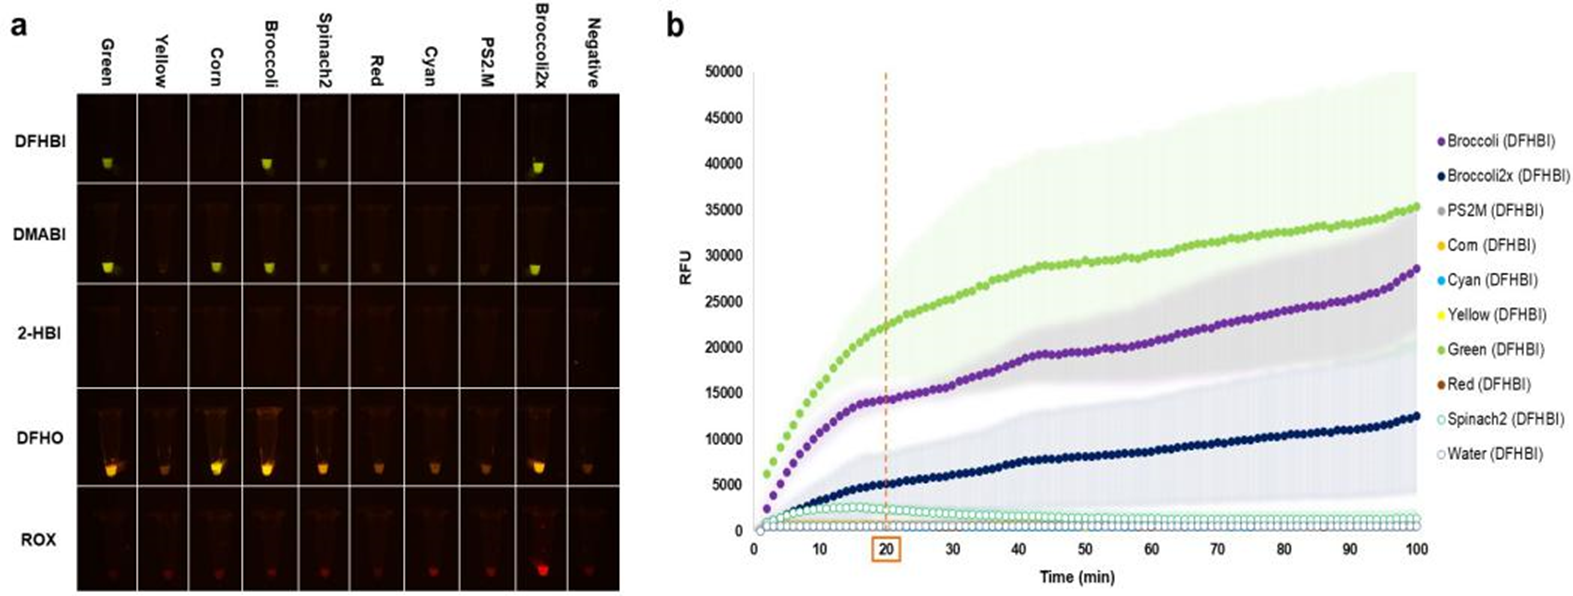
\includegraphics[height=140px, width=300px]{chapter2/chapter/figs/Imagen2.png}
\end{center}
\caption{Fluorescent RNA aptamers expression. \textbf{(a)} Aptamers showing different colours under a blue light/red filter system after plate reader fluorescent measurement (16.5 h) and being observed by naked eye without the need for further equipment. A longer exposed image can be found in Figure \ref{fig34}.
\textbf{(b)} Expression of diverse RNA aptamers over time detected at 480/520 nm. Coloured shades represent the variability (MAD) of three independent tests. }
\label{NAR-fig2}
\end{figure*}

\subsection*{TXO cell-free biosensors}
Short aptamers such as the Green aptamer allow incorporation into transcriptional units with ease and simplicity (see Materials and Methods). Considering the stability and optimization of the Green aptamer (F30::iSpinach) for expression under in vitro conditions, further experiments were performed with this aptamer. The Green aptamer (F30::iSpinach) was amplified via PCR under the control of diverse heavy metal inducible promoters and the T7 polymersase promoter as control (P$_{t7}$, P$_{cue}$, P$_{ars}$, P$_{mer}$, P$_{pbr}$, P$_{czc}$, P$_{cnr}$, see Material and Methods). Linear PCR products were used in reactions with different heavy metal concentrations (5 $\mu$M, 25 $\mu$M and 100 $\mu$M) with transcription factors and native RNA polymerase supplied from cell lysates (see Figure \ref{NAR-fig3}). Using our TXO cell free system concentrations as low as 2 $\mu$M were detected for lead, mercury, zinc, and arsenite. Nickel, on the other hand, was detected at 0.3 $\mu$M. All of them reached a 2 fold-change in fluorescence after just 20 min of initiation of the transcription reaction (see Figure \ref{NAR-fig3}) which kept increasing over time reaching after three hours values up to 10-times higher (see Figure \ref{NAR-figS2}).

\begin{figure*}[t]
\begin{center}
\hspace*{0cm}
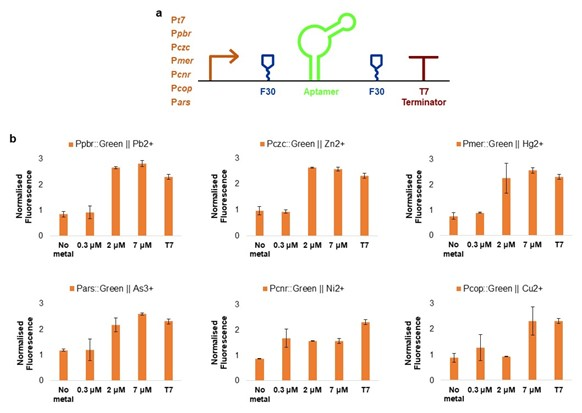
\includegraphics[width=380px]{chapter2/chapter/figs/Imagen3.jpg}
\end{center}
\caption{Heavy metal detection by TXO Cell-free biosensors. Detection of Pb$^{2+}$, Hg$^{2+}$, Zn$^{2+}$, Ni$^{2+}$, Cu$^{2+}$ and As$^{3+}$
using the TXO reaction Cell-free system and the Green RNA aptamer cloned with each specified promoter (P\textit{pbr}, P\textit{mer}, P\textit{cnr}, P\textit{czc}, P\textit{cop}, and P\textit{ars}). Constructs were induced using increasing concentrations of the specified heavy-metal. Excitation/Emission of 480/520 nm. Data points at 20 minutes; the time course can be found in Figure \ref{NAR-figS2}. Error bars represent the variability (MAD) of three independent tests.}
\label{NAR-fig3}
\end{figure*}


\section{Discussion / Conclusions}
TXO systems maintain the advantages of cell-free TX-TL systems in terms of uniformity and avoidance of regulatory issues related to live GMOs, and further increase the simplicity and speed of response at the expense of reduced flexibility, since new proteins can not be generated within the system. Hence, they are well suited to applications where simplicity and rapid response are paramount; for example, biosensors and diagnostics for use in field and point-of-care applications. Lack of translational capability means that reporters for system output must be in the form of nucleic acids. We tested eight previously described fluorescent aptamer-fluorophore systems and found that all could generate visible fluorescent responses in an optimized buffer system as a result of transcription with no further processing. Several of the aptamers showed the ability to bind a wider range of fluorophores than what has previously been reported; for example, Broccoli2X binds 4 out of the 5 fluorophores analysed (Figure \ref{NAR-fig2}a and \ref{fig34}), surprisingly including ROX (5-Carboxy-X-rhodamine N-succinimidyl ester) commonly used for basal line generation during routine fluorescent assays, such as qPCR. Using TXO systems fluorescent responses can be generated in a matter of minutes, as compared to an hour or more for reported TX-TL systems based on generation of fluorescent proteins or enzymes with chromogenic substrates \citep{borkowski2016overloaded,bernhard2013cell,carlson2012cell,kwon2015high,salehi2017cell,salehi2018biosensing}. Thus, we conclude that aptamer-fluorophore complexes are a suitable output for TXO synthetic biology systems.
A further advantage of TXO systems is simplicity, meaning that they can be very rapidly generated and tested, even more so than TX-TL systems \citep{pardee2016rapid}. The aptamer-based reporter genes are small enough that they can be easily generated by annealing and extension of oligonucleotides (see Figure \ref{NAR-fig1}). PCR was used to add metal-responsive promoters to DNA encoding the F30::iSpinach reporter (‘Green’), and the PCR products were used directly for assays, with the necessary transcription factors being supplied by an unpurified lysate from \textit{C. metallidurans} CH34. Fluorescent response to metals was observed within minutes, with detection limits in these unoptimized systems below 0.3 $\mu$M (18 ppb) for nickel, below 2 $\mu$M for zinc (131 ppb), arsenic(III) (150 ppb), mercury (403 ppb) and lead (414 ppb) and 7 uM for copper (127 ppb). No response was observed for arsenic(V), presumably because the system lacked the reducing power necessary to reduce it to arsenic(III), the form actually detected by the ArsR repressor (Data not shown). Further optimization should reduce these limits of detection. Previous works with RNA aptamers for metal sensing, DasGupta et al. mentioned the use of a truncated form of the Spinach aptamer as a Pb2+ sensor, but this could have lead to false results at concentrations <2 ppm due to a lack of sensitivity and a weak output response \citep{alam2017fluorescent}.
Since TXO systems are considerably simpler than TX-TL systems, with no requirement for ribosomes, tRNA, or associated enzymes, we expect that it will be possible to freeze-dry such systems for storage and distribution as previously reported for TX-TL systems \citep{grawe2019paper,pardee2014based}. Fluorescent signals may be further strengthened using alternative fluorophores such as DHFBI-1T \citep{song2014plug}. The visibly different colours, as well as different excitation and emission wavelengths for different aptamer-fluorophore complexes, raise the possibility of multiplexed assays as well as more complex approaches such as FRET and quenching. While this publication focuses on the use of aptamers as signal output in a TXO ststem, future research could exploit the advantages of translation independent systems introducing other known functions of RNA molecules. Examples include RNA-based molecule detection (e.g. using riboswitch aptamers) and signal processing (e.g. using RNA-RNA hybridisation networks or crRNA/gRNA) \citep{alam2017fluorescent, DasGupta2015a, etzel2017synthetic, patel2018synthetic, rodrigo2017model, jaffrey2018rna}. Possible improvements to the already existing technology could also imply the use of other RNA aptamers showing different properties, for instance, by improving the structure and conditions of other aptamers published in the original work by Paige et al, which emit fluorescence in different wavelength, i.e. red, yellow, cyan (see Table \ref{table:3.1} and Figure \ref{NAR-fig2}) or by using ribozymes, such as PS2.M, allowing additional possible transcriptional outputs and broadening the possibilities of TXO systems.
Additionally, TXO systems can be made with no need for GMOs, using in vitro DNA manipulation and non-ionic detergent lysis of wild type ACDPI or Biosafety level 1 cells, plus non toxic chemicals and commercially available enzymes/proteins, so so procedures could easily be done in high schools or even at home, leading to a democratization of synthetic biology without the worrying risks of people making bioweapons or causing ecological disasters. Considering that algorithms are simply a sequence of instructions, typically to solve a class of problems or perform a computation, TXO systems offer a step forward in terms of simplicity, ease of implementation, and rapid response, and may be widely useful in synthetic biology for speeding up and simplifying genetic circuit algorithm design and response.



\section{Data Availability}
All datasets generated for this study are included in the manuscript and/or the supplementary files. More Data is available at 

\section{Acknowledgments}

  
The authors acknowledge the valuable assistance of Dr. Samie R Jaffrey on providing diverse RNA aptamers and fluorophores, Dr. Michael Ryckelynck for providing the iSpinach aptamer and Dr. Simon J. Moore for his help in the cell-free system design. Authors also acknowledge the following funding sources: CONICYT/BC-PhD 72170403 (FM), Biotechnology and Biological Sciences Research Council (BBSRC) [grant number BB/J01446X/1] (MV). A pre-print version of the manuscript has been published on BioRxiv (Millacura et al., 2019).

\section{Supplementary Material}


\begin{table}[ht]
%\captionsetup{labelformat=empty}
\caption{Fluorophores information\\}
\label{table:32}%
{%\hspace*{-5cm}
\begin{tabular*}{\columnwidth}{@{}lll@{}}
\hline
Abbreviation & Formula & Chemical name 
\\
\hline
DFHBI & C$_{12}$H$_{10}$F$_{2}$N$_{2}$O$_{2}$ &  3,5-difluoro-4-hydroxybenzylidene 
\\
& &  imidazolinone
\\
DMABI* & C$_{14}$H$_{17}$N$_{3}$O$_{1}$ & 4-dimethylaminobenzylidene imidazo-
\\
&  & linone
\\
2-HBI* & C$_{12}$H$_{12}$N$_{2}$O$_{2}$ &  2-hydroxybenzlidene imidazolinone  
\\
DFHO & C$_{12}$H$_{9}$F$_{2}$N$_{3}$O$_{3}$ & 3,5-difluoro-4-hydroxybenzylidene 
\\
&  & imidazolinone-2-oxime
\\
ROX & C$_{37}$H$_{33}$N$_{3}$O$_{7}$ & 5-Carboxy-X-rhodamine N-succinimidyl  
\\
&  & ester
\\
\hline
\hline
\end{tabular*}
}
\\
{\footnotesize{*provided by Dr. Sammie R. Jaffrey's laboratory}}
\end{table}

\begin{figure*} [ht] 
\begin{center}
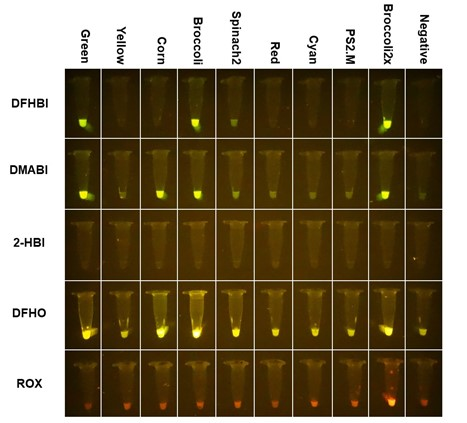
\includegraphics[width=350px]{chapter2/chapter/figs/Imagen4.jpg}
\end{center}
%\captionsetup{labelformat=empty}
\caption{Fluorescent RNA aptamers observed under a blue  light/red  filter  system. Aptamers  showing  different  colours  under  a  blue  light/red  filter  system  after measurement 16.5 h and being observed by naked eye without the need for further equipment. Picture taken with a Sony, DSC-RX100 camera and aperture}
\label{fig34}%
\end{figure*}

\begin{table}[ht]
%\captionsetup{labelformat=empty}
\caption{Oligonucleotides used\\}
\label{table:331}%
{%\hspace*{-4cm}
\begin{tabular*}{\columnwidth}{@{}lll@{}}
\hline
\textbf{Oligo} & \textbf{Name} & \textbf{Sequence}
\\
\\
\hline
F240 & Cyan$_{F30::2-4}Fw$ &  \MakeLowercase{TGTGGGAGACGCAACTGAATGAACCTAGAGTTATGCCAGG}
\\
& & \MakeLowercase{CTCTGAGCCTGCTTCGGCAGGTGCTATGATCGCCAGCGGTA}
\\
& & \MakeLowercase{TGCAGTCCGTAACTAGTCGCGTCTCC}
\\
F241 & Cyan$_{F30::2-4}Rv$ &  \MakeLowercase{GTGGGGAGACGCGACTAGTTACGGACTGCATACCGCTGGC}
\\
& & \MakeLowercase{GATCATAGCACCTGCCGAAGCAGGCTCAGAGCCTGGCATA}
\\
& & \MakeLowercase{ACTCTAGGTTCATTCAGTTGCGTCTCC}
\\
F242 & 	Red$_{F30::6-8}Fw$ &  \MakeLowercase{TGTGGGagacgcaactgaatgaaaatggcaaaatattcga}
\\
 & &  \MakeLowercase{gaagctggtctgcttcggcaggattctccaaggggtagatc}
\\
& & \MakeLowercase{gtgtattccgtaactagtcgcgtcTCC}
\\
F243 & Red$_{F30::6-8}Rv$ &  \MakeLowercase{GTGGGgagacgcgactagttacggaatacacgatctaccc}
\\
& & \MakeLowercase{cttggagaatcctgccgaagcagaccagcttctcgaatatt}
\\
& & \MakeLowercase{ttgccattttcattcagttgcgtcTCC}
\\
F244 & Yellow$_{F30::17-3}Fw$ &  \MakeLowercase{TGTGGGagacgcaactgaatgaagagcagtagcgagtag}
\\
& & \MakeLowercase{ttcacaagagctgcttcggcaggatcttgtaggaagtaaat}
\\
& & \MakeLowercase{gtgcaaatccgtaactagtcgcgtctcC}
\\
F245 & Yellow$_{F30::17-3}Rv$ &  \MakeLowercase{GTGGGgagacgcgactagttacggatttgcacatttacttc}
\\
& & \MakeLowercase{ctacaagatcctgccgaagcagctcttgtgaactactcgc}
\\
& & \MakeLowercase{tactgctcttcattcagttgcgtctCC}
\\
F296 & Green$_{F30::iSpinach}Fw$ &  \MakeLowercase{gaattcgcggccgcttCTAGAGTAATACGACTCACTATAG}
\\
&  &  \MakeLowercase{GGTTGCCATGTGTATGTGGGAGACGCGACTACGGTGAGGG}
\\
&  &  \MakeLowercase{TCGGGTCCAGTAGCTTCGGCTACTGTTGAGTAGAGTGTGG}
\\
F297 & Green$_{F30::iSpinach}Rv$ & \MakeLowercase{ctgcagcggccgctactagtaCCCCTCAAGACCCGTTTAG}
\\
&  &  \MakeLowercase{AGGCCCCAAGGGGTTATTTGCCATGAATGATCCCGAAGGA}
\\
&  &  \MakeLowercase{TCATCAGAGTATGTGGGGAGACGTACGGAGCCCACA}
\\
F310 & P$_{pbr}$::Green Fw &  \MakeLowercase{GAATTCGCGGCCGCTTCTAGAGGGCGTCGGATGGGAGATG}
\\
&  &  \MakeLowercase{TCTTGACTCTATAGTAACTAGAGGGTGTTAAATCGGCAACT}
\\
&  &  \MakeLowercase{TGCCATGTGTATGTGGGAGACGCGACTACGGTGAGGGTC}
\\
F311 & P$_{mer}$::Green Fw & \MakeLowercase{GAATTCGCGGCCGCTTCTAGAGATCGCTTGACTCCGTACAT}
\\
& & \MakeLowercase{GAGTACGGAAGTAAGGTTACGCTATCCAATTTCAATTCGA}
\\
& & \MakeLowercase{ATTGCCATGTG}
\\
F312 & P$_{cop}$::Green Fw & \MakeLowercase{GAATTCGCGGCCGCTTCTAGAGAATTTCTTGACCTTCCCCT}
\\
& & \MakeLowercase{TGCTGGAAGGTTTAACCTTTATCACATTGCCATGTGTATGT}
\\
& & \MakeLowercase{GGGAGACGCG}
\\
F313 & P$_{ars}$::Green Fw & \MakeLowercase{GAATTCGCGGCCGCTTCTAGAGGTATATACACATTCGTTA}
\\
 &  & \MakeLowercase{AGTCATATATGTTTTTGACTTATCCGCTTCGAAGAGAGAC}
\\
&  & \MakeLowercase{ACTACCTGCAACTTGCCATGTGTATGTGGGAGACGCGACT}
\\
F330 & Corn$_{F30::Corn}Fw$ & \MakeLowercase{GATCCTTCGGGATCATTCATGGCAAATAACCCCTTGGGGC}
\\
& & \MakeLowercase{CTCTAAACGGGTCTTGAGGGGTACTAGTAGCGGCCGCTG}
\\
&& \MakeLowercase{CAGtactata}
\\
F331 & Corn$_{F30::Corn}$Rv & \MakeLowercase{CTCCTCAGACCTCCTTCCTCGCGCcgtctCCCACATACAC}
\\
& & \MakeLowercase{ATGGCAACCCTATAGTGAGTCGTATTACTCTAGaagcgg}
\\
&& \MakeLowercase{ccgcgaattc}
\\
\hline
\end{tabular*}
}{ }
\end{table}

\newpage
\makeatletter
\setlength{\@fptop}{0pt}
\makeatother
\begin{table}[ht!]
\label{table:332}
{%\hspace*{-4cm}
\begin{tabular*}{\columnwidth}{@{}lll@{}}
\hline
\textbf{Oligo} & \textbf{Name} & \textbf{Sequence}
\\
\\
\hline
F404 & 	P$_{czcN}$::GreenFw & \MakeLowercase{GAATTCGCGGCCGCTTCTAGAGggagggcgtctctg}
\\
&  &  \MakeLowercase{ggtgtgtgctgaaaatggccaagacagtctatgtcc}
\\
&  &  \MakeLowercase{cagaagatgactgtcagattgccgagctTTGCCATG}
\\
&  &  \MakeLowercase{TGTATGTGGGAG}
\\
F405 & P$_{cnr}$::GreenFw & \MakeLowercase{GAATTCGCGGCCGCTTCTAGAGggaggcctgaagc}
\\
& & \MakeLowercase{cggaacatcgacctgcttacgatcgcgttcttatcg}
\\
& & \MakeLowercase{atgcacTTGCCATGTGTATGTGGGAGACG}
\\
F408 & PS2M$_Fw$ & \MakeLowercase{gaattcgcggccgcttCTAGAGTAATACGACTCACT}
\\
&  &  \MakeLowercase{ATAGGGGTGGGTAGGGCGGGTTGGATAACCCCTTG}
\\
&  &  \MakeLowercase{GGGCCTCTAAACGGGTCCTTGAGGGGtactagtagc}
\\
& & \MakeLowercase{ggccgctgcagTAT}
\\
F409 & PS2M$_Rv$ & \MakeLowercase{ATActgcagcggccgctactagtaCCCCTCAAGAC}
\\
& & \MakeLowercase{CCGTTTAGAGGCCCCAAGGGGTTATCCAACCCGCC}
\\
& & \MakeLowercase{CTACCCACCCCTATAGTGAGTCGTATTACTCTAGaa}
\\
& & \MakeLowercase{gcggccgcgaattc}
\\
F296-F297 & BBK::P$_{T7}$::Green & \MakeLowercase{gaattcgcggccgcttCTAGAGTAATACGACTCACT}
\\
& ::T$_{T7}$::BBK& \MakeLowercase{ATAGGGTTGCCATGTGTATGTGGGAGACGCGACTAC}
\\
& & \MakeLowercase{GGTGAGGGTCGGGTCCAGTAGCTTCGGCTACTGTTG}
\\
& & \MakeLowercase{AGTAGAGTGTGGGCTCCGTAGTCGCGTCTCCCCACA}
\\
&  & \MakeLowercase{TACTCTGATGATCCTTCGTCGGGTCCAGTAGCTTCGG}
\\
&  & \MakeLowercase{CTACTGTTGAGTAGAGTGTGGGCTCCGTAGTCGCGTC}
\\
& & \MakeLowercase{TCCCCACATACTCTGATGATCCTTCGGGATCATTCAT}
\\
& & \MakeLowercase{GGCAAATAACCCCTTGGGGCCTCTAAACGGGTCTTG}
\\
& & \MakeLowercase{AGGGGtactagtagcggccgctgcag}
\\
F313-F297 & BBK::P$_{ars}$::Greeen & \MakeLowercase{GAATTCGCGGCCGCTTCTAGAGGTATATACACATTC}
\\
& ::T$_{T7}$::BBK & \MakeLowercase{GTTAAGTCATATATGTTTTTGACTTATCCGCTTCGAAG}
\\
& & \MakeLowercase{AGAGACACTACCTGCAACTTGCCATGTGTATGTGGG}
\\
& & \MakeLowercase{AGACGCGACTACGGTGAGGGTCGGGTCCAGTAGCT}
\\
& & \MakeLowercase{TCGGCTACTGTTGAGTAGAGTGTGGGCTCCGTAGTCG}
\\
&& \MakeLowercase{CGTCTCCCCACATACTCTGATGATCCTTCGGGATCAT}
\\
& & \MakeLowercase{TCATGGCAAATAACCCCTTGGGGCCTCTAAACGGG}
\\
& & \MakeLowercase{TCTTGAGGGGtactagtagcggccgctgcag}
\\
F405-F297 & BBK::P$_{cnr}$::Green & \MakeLowercase{GAATTCGCGGCCGCTTCTAGAGggaggcctgaagc}
\\
& ::T$_{T7}$::BBK & \MakeLowercase{cggaacatcgacctgcttacgatcgcgttcttatcg}
\\
& & \MakeLowercase{atgcacTTGCCATGTGTATGTGGGAGACGCGACTAC}
\\
& & \MakeLowercase{GGTGAGGGTCGGGTCCAGTAGCTTCGGCTACTGTTG}
\\
& & \MakeLowercase{AGTAGAGTGTGGGCTCCGTAGTCGCGTCTCCCCACA}
\\
&&\MakeLowercase{TACTCTGATGATCCTTCGGGATCATTCATGGCAAATA}
\\
& & \MakeLowercase{ACCCCTTGGGGCCTCTAAACGGGTCTTGAGGGGtac}
\\
& & \MakeLowercase{tagtagcggccgctgcag}
\\



\hline
\end{tabular*}
} { }
\end{table}

\newpage
\makeatletter
\setlength{\@fptop}{0pt}
\makeatother
\begin{table}[ht!]
\label{table:333}
{%\hspace*{-4cm}
\begin{tabular*}{\columnwidth}{@{}lll@{}}
\hline
\textbf{Oligo} & \textbf{Name} & \textbf{Sequence}
\\
\\
\hline
F312-F297 & BBK::P$_{cop}$::Green & \MakeLowercase{GAATTCGCGGCCGCTTCTAGAGAATTTCTTGACCTTCC}
\\
& ::T$_{T7}$::BBK & \MakeLowercase{CCTTGCTGGAAGGTTTAACCTTTATCACATTGCCATGT}
\\
&  & \MakeLowercase{GTATGTGGGAGACGCGACTACGGTGAGGGTCGGGTC}
\\
&  & \MakeLowercase{CAGTAGCTTCGGCTACTGTTGAGTAGAGTGTGGGCTC}
\\
& & \MakeLowercase{CGTAGTCGCGTCTCCCCACATACTCTGATGATCCTTCG}
\\
& & \MakeLowercase{GGATCATTCATGGCAAATAACCCCTTGGGGCCTCTAA} 
\\
& & \MakeLowercase{ACGGGTCTTGAGGGGtactagtagcggccgctgcag} 
\\
F404-F297 & BBK::P$_{czc}$::Green & \MakeLowercase{GAATTCGCGGCCGCTTCTAGAGggagggcgtctctgg}
\\
&::T$_{T7}$::BBK & \MakeLowercase{gtgtgtgctgaaaatggccaagacagtctatgtccca}
\\
& & \MakeLowercase{gaagatgactgtcagattgccgagctTTGCCATGTGTA}
\\
& & \MakeLowercase{TGTGGGAGACGCGACTACGGTGAGGGTCGGGTCCAG}
\\
& & \MakeLowercase{TAGCTTCGGCTACTGTTGAGTAGAGTGTGGGCTCCGTA}
\\
& & \MakeLowercase{GTCGCGTCTCCCCACATACTCTGATGATCCTTCGGGAT}
\\
&&\MakeLowercase{CATTCATGGCAAATAACCCCTTGGGGCCTCTAAACG}
\\
& & \MakeLowercase{GGTCTTGAGGGGtactagtagcggccgctgcag}
\\
F311-F297 & BBK::P$_{mer}$::Green & \MakeLowercase{GAATTCGCGGCCGCTTCTAGAGATCGCTTGACTCCGT}
\\
& ::T$_{T7}$::BBK& \MakeLowercase{ACATGAGTACGGAAGTAAGGTTACGCTATCCAATTT}
\\
&  & \MakeLowercase{CAATTCGAATTGCCATGTGTATGTGGGAGACGCGAC}
\\
& & \MakeLowercase{TACGGTGAGGGTCGGGTCCAGTAGCTTCGGCTACTG}
\\
&& \MakeLowercase{TTGAGTAGAGTGTGGGCTCCGTAGTCGCGTCTCCCCA}
\\
& & \MakeLowercase{CATACTCTGATGATCCTTCGGGATCATTCATGGCAAA}
\\
& & \MakeLowercase{TAACCCCTTGGGGCCTCTAAACGGGTCTTGAGGGGt}
\\
& & \MakeLowercase{actagtagcggccgctgcag}
\\
F310-F297 & BBK::P$_{pbr}$::Green & \MakeLowercase{GAATTCGCGGCCGCTTCTAGAGGGCGTCGGATGGGA}
\\
& ::T$_{T7}$::BBK & \MakeLowercase{GATGTCTTGACTCTATAGTAACTAGAGGGTGTTAAAT}
\\
& & \MakeLowercase{CGGCAACTTGCCATGTGTATGTGGGAGACGCGACTA}
\\
& & \MakeLowercase{CGGTGAGGGTCGGGTCCAGTAGCTTCGGCTACTGTTG}
\\
&& \MakeLowercase{AGTAGAGTGTGGGCTCCGTAGTCGCGTCTCCCCACA}
\\
& & \MakeLowercase{TACTCTGATGATCCTTCGGGATCATTCATGGCAAATA}
\\
& & \MakeLowercase{ACCCCTTGGGGCCTCTAAACGGGTCTTGAGGGGtaC}
\\
& & \MakeLowercase{tagtagcggccgctgcag}
\\
\hline
\hline
\end{tabular*}
} { }
\end{table}


\begin{figure*} [ht] 
\begin{center}
%\hspace*{-2.5cm}
\includegraphics[width=500px]{chapter2/chapter/figs/figureS2.png}
\end{center}
%\captionsetup{labelformat=empty}
\caption{TXO sensors over time with different metals. Coloured shades represent variability of three independent tests.}
\label{NAR-figS2}%
\end{figure*}

\renewcommand{\dir}{../chapter3/chapter/}
\chapter{Unintentional Genomic Changes Endow \textit{Cupriavidus metallidurans} with an Augmented Heavy-Metal Resistance }

\section{Foreword}

While looking into the diverse abilities present in the genome of \textit{Cupriavidus metallidurans}, it was observed that mutants of this bacteria are difficult to make or too unstable. A natural plasmid pTP6 was previously introduced into strain CH34, increasing its resistance to mercury. However, resistance to some other heavy metals were also increased but with no direct relation to the resistance markers introduced. After genomic sequencing, it was observed that this bacteria has an inherit genetic unstability allowing it to adapt under harsh conditions. 

The present chapter has been published as a research article entitled “Unintentional Genomic Changes Endow \textit{Cupriavidus metallidurans} with an Augmented Heavy-Metal Resistance” in the peer-reviewed journal Genes. Sections from 4.2 to 4.9 show the published manuscript including its Supplementary Information. Additional information, official links and repositories are mentioned within the chapter text. 

\section{Abstract}

For the past three decades, \textit{Cupriavidus metallidurans} has been one of the major model organisms for bacterial tolerance to heavy metals. Its type strain CH34 contains at least 24 gene clusters distributed over four replicons, allowing for intricate and multilayered metal responses. To gain organic mercury resistance in CH34, broad-spectrum \textit{mer} genes were introduced in a previous work via conjugation of the IncP-1$\beta$ plasmid pTP6. However, we recently noted that this CH34-derived strain, MSR33, unexpectedly showed an increased resistance to other metals (i.e., Co$^{2+}$, Ni$^{2+}$, and Cd$^{2+}$). To thoroughly investigate this phenomenon, we resequenced the entire genome of MSR33 and compared its DNA sequence and basal gene expression profile to those of its parental strain CH34. Genome comparison identified 11 insertions or deletions (INDELs) and nine single nucleotide polymorphisms (SNPs), whereas transcriptomic analysis displayed 107 differentially expressed genes. Sequence data implicated the transposition of IS1088 in higher Co$^{2+}$ and Ni$^{2+}$ resistances and altered gene expression, although the precise mechanisms of the augmented Cd$^{2+}$ resistance in MSR33 remains elusive. Our work indicates that conjugation procedures involving large complex genomes and extensive mobilomes may pose a considerable risk toward the introduction of unwanted, undocumented genetic changes. Special efforts are needed for the applied use and further development of small nonconjugative broad-host plasmid vectors, ideally involving CRISPR-related and advanced biosynthetic technologies.

\section{Introduction}

Since life appeared on earth some 3.7 billion years ago, microorganisms have undergone molecular changes to adapt (i.e., respond to selection) to the harsh conditions of their natural habitats, including extreme temperatures, pH, salinity, UV and ionizing radiation, and heavy metals \citep{bakermans2015microbial}. In addition, global fluctuations in the composition of the atmosphere, the oceans, and the earth crust have elicited genomic changes in microbes over eons of time and hence contributed to microbial diversity \citep{knoll2015paleobiological}. Certain microorganisms had been adapted to heavy metals and radionuclides prior to human appearance. However, during the past few hundred years, anthropogenic influences have forced microbes to also adapt to pollutants previously nonexistent (xenobiotics) \citep{springael2004horizontal, cao2012characterization, ilori2015catabolic, mergeay2014adaptation}, as well as to increased concentrations of heavy metals and radionuclides \citep{nies1999microbial, mergeay2000bacteria, sobecky2009horizontal}.
Members of the \textit{beta}-proteobacterial genus \textit{Cupriavidus} are prime examples of microbial endurance, possessing a variety of genomic islands involved in the resistance to heavy metals or the degradation of aromatics or xenobiotics \citep{pohlmann2006genome, amadou2008genome, janssen2010complete, lykidis2010complete, poehlein2011complete,cserhati2012novo, hong2012whole, li2013genome, ray2015complete, wang2015genome, fang2016complete}. They all typically display a bipartite chromosomal structure with one chromosomal replicon bearing the marks of a plasmid-type maintenance and replication system henceforth called “chromid”. In addition, most \textit{Cupriavidus} strains carry one or two dispensable megaplasmids with a size of 100 kb or more. The model organism for heavy metal resistance, \textit{Cupriavidus metallidurans} strain CH34, carries two megaplasmids, pMOL28 and pMOL30. Together, the four CH34 replicons encode resistance markers for a plethora of heavy metals including copper, nickel, zinc, cobalt, cadmium, chrome, lead, silver, gold, mercury, caesium, selenium, strontium, and uranium \citep{janssen2010complete, mergeay2003ralstonia, monchy2007plasmids, avoscan2007uranium, monsieurs2011heavy, salem2013strontium}. These resistances are mainly related to a variety of metal reduction and efflux systems \citep{van2015genomic, vandenbussche2015metal,nies2016biological}. Aromatics degradation, on the other hand, is carried out by various bacterial multicomponent mono- and di-oxygenases solely encoded by genes on the chromosome and chromid \citep{millacura2017degradation}.
In an effort to improve the inorganic and organic mercury resistance of \textit{C. metallidurans} CH34 and thus improve its utility in cleaning up mercury-contaminated environments, the IncP-1$\beta$ plasmid pTP6, providing additional \textit{mer} genes \citep{smalla2006increased}, was introduced in CH34 by biparental mating, leading to strain MSR33 \citep{rojas2011characterization}. These extra \textit{mer} genes are part of a transposon, Tn50580, which is necessary for broad-spectrum (organomercury) resistance, including two genes, \textit{merG} and \textit{merB}, not native to CH34 (i.e., CH34 only contains two narrow-spectrum mercury resistance \textit{merRTPADE} operons, one on each megaplasmid, conferring resistance to inorganic mercury). MerB plays a key role in methylmercury degradation through its unique ability to cleave the carbon-mercury bond in methylmercury and the subsequent shuttling of ionic mercury to MerA to reduce it to the less harmful elemental mercury.
In comparison to its parental strain CH34, strain MSR33 became 240\% more resistant to inorganic mercury and gained resistance to methylmercury by incorporating the previously nonpresent \textit{merBG} genes. Other metal resistances (as tested for chrome and copper) were seemingly unaffected, and the pTP6 plasmid was stably maintained for over 70 generations under nonselective pressure \citep{rojas2011characterization}. However, when we recently tested the resistances for both strains to additional metals (i.e., cadmium, cobalt, and nickel), we noted a significant increase of metal resistance for strain MSR33 compared to CH34 (this study). As this was fully unexpected, since the only difference between the two strains should be an additional \textit{mer} gene dosage, implicating only an improved mercury resistance, we set out to investigate the reasons for this phenomenon. Considering the genome plasticity \citep{van2009new,mijnendonckx2011insertion,van2012variation} and the intricate relationships between metal resistance loci \citep{monsieurs2011heavy} in \textit{C. metallidurans} CH34, we decided to sequence the full genome of strain MSR33 and compare the sequence of its replicons with the corresponding replicons of the parental strain CH34 and with plasmid pTP6. We also performed microarray-based expression analysis on both CH34 and MSR33 gene sets to determine whether genomic differences could be correlated with differences in the expression of individual genes.

\section{Materials and Methods}

\subsection{Strains and Culture Conditions}

\textit{Cupriavidus metallidurans} strains CH34 and MSR33, obtained from respectively the SCK$\cdot$CEN (Mol, Belgium) and the Univesidad Católica del Norte (UCN) (Antofagasta, Chile) culture collections, were cultivated at 30$^{\circ}$C and 200 revolutions per minute (rpm) on a shaker in dark, aerobic conditions in a Tris-buffered mineral medium (MM284) \citep{mergeay1985alcaligenes} with 0.4\% (w/v) succinate as the sole carbon source. Escherichia coli JM109 pTP6 (also obtained from the UCN culture collection) was cultured at 37$^{\circ}$C on an M9 minimal medium \citep{sambrook1989molecular} supplemented with 0.4\% (w/v) glucose.

\subsection{Synthetic Construct Generation}

The \textit{merTPAGB1} gene cluster of pTP6 was amplified by PCR using Phusion High-Fidelity DNA polymerase (ThermoFisher, Aalst, Belgium) with primer pair pTP6mer$_{Fw-Rv}$ (Table \ref{table:44}). In tandem, the broad-host-range cloning vector pBBR1MCS-2 \citep{kovach1995four} was linearized by PCR with the same DNA polymerase and primer pair pBBR1MCS-2-GA$_{Fw-Rv}$ (Table \ref{table:44}), providing homologous ends with the amplified \textit{merTPAGB1} locus. These compatible PCR products were end-ligated using the Invitrogen GeneArt \textsuperscript{\tiny\textregistered} Seamless Cloning and Assembly Enzyme Mix (ThermoFisher). After transforming \textit{E. coli} DG1 with the ligation mix and selection on Lysogeny Broth (LB) with 50 $\mu$g/mL kanamycin (Km), four randomly chosen transformants were tested by DNA digestion and fragment sizing for correct plasmid construction holding the \textit{merTBAGB1} genes. The plasmid gene construct of one transformant was further verified by sequencing its insert using forward and reverse cloning primers (Table \ref{table:44}) prior to electroporation into \textit{C. metallidurans} CH34 on an Eppendorf 2510 Electroporator (Eppendorf, Aarschot, Belgium) using conditions as described previously \citep{taghavi1994electroporation}.

\subsection{Estimation of Bacterial Tolerance to Metals}

Strains CH34 and MSR33 were grown overnight in MM284 liquid media with 0.4\% (w/v) succinate as the sole carbon source and thereafter used as a pre-inoculum (1\% v/v) for a freshly prepared 200 $\mu$L culture supplemented with increased concentrations of Hg$^{2+}$ (from 0.0625 mM to 8 mM), Cd$^{2+}$ (from 0.25 mM to 8 mM), and increasing steps (1 mM) of Co$^{2+}$ or Ni$^{2+}$ (from 5 mM to 20 mM). Cultures for metal contact were grown in microtiter plates at 30$^{\circ}$C on a rotary shaker at 120 rpm. Metal ion solutions were prepared from soluble salts of analytical grade (CdCl$_{2+}$, HgCl$_{2+}$, CoCl$_{2+}$·6H$_{2+}$O, and NiCl$_{2+}$·6H$_{2+}$O) in double-deionized water and were filter-sterilized before use. The lowest metal concentration that prevented growth after 48 h (i.e., showing no growth as measured at OD600 by a CLARIOstar microplate reader (BMG LabTech, Offenburg, Germany)), was considered the minimum inhibitory concentration (MIC) (Table \ref{table:41} and Table \ref{table:45}). All MIC analyses were performed using biological triplicates.

\begin{table}[ht]
%\captionsetup{labelformat=empty}
\caption{Minimal inhibitory concentration (MIC) of heavy metals for \textit{Cupriavidus metallidurans} strains MSR33 and CH34. \\ }
\label{table:41}%
{%\hspace*{-4cm}
\begin{tabular*}{\columnwidth}{@{}lllll@{}}
\hline
\textbf{Strain/Metal in mM} & \textbf{Hg$^{2+}$} & \textbf{Cd$^{2+}$} & \textbf{Ni$^{2+}$} & \textbf{Co$^{2+}$} \\
\hline
				
\textit{C. metallidurans }CH34 &	0.01 &	2.0 & 10.0 & 11.0 \\
\textit{C. metallidurans} MSR33 & 0.10 &	4.0 & 12.0 & 20.0 \\
\textit{C. metallidurans} CH34 (pBBR::\textit{merTPAGB1}) &	0.10 &	2.0	& ND$^1$ &	ND$^1$ \\
\\
\hline
\hline
\end{tabular*}
} {\footnotesize{$^1$ND: not determined.}}

\end{table}


\subsection{Plasmid Copy Number Determination}

Single-copy (i.e., “replicon-unique”) genes were taken as representatives of the chromosome (\textit{cadA}), chromid (\textit{zniA}), and plasmids pMOL30 (\textit{nccA}), pMOL28 (\textit{cnrA}), and pTP6 (\textit{merG}). Primer pairs were designed to amplify 150 bp of each gene (Table \ref{table:44}). Real-time PCR was performed on a 7500 Applied Biosystems Fast Real-Time PCR System (ThermoFisher) using QiaGen RT2 Sybr Green Rox qPCR Mastermix (ThermoFisher), 20 ng of MSR33 or CH34 genomic DNA as a template, and 0.2 $\mu$M of each primer. To reduce nonspecific amplification, we incubated this mixture at 95 $^{\circ}$C for 10 min as part of a hot start PCR setup. Next, a 40-cycle amplification and quantification protocol (15 s at 95 $^{\circ}$C, 15 s at 58 $^{\circ}$C, and 30 s at 60 $^{\circ}$C) was performed with a single fluorescence measurement for each cycle. Finally, a melting curve program (15 s at 95 $^{\circ}$C, 60 s at 60 $^{\circ}$C, 30 s at 95 $^{\circ}$C, and 15 s at 60 $^{\circ}$C) was carried out. Plasmid copy numbers for both strains were determined using the absolute method (allowing estimates of both the absolute and relative number of plasmids per cell), following earlier described protocols \citep{lee2006absolute}. Standard curves were created with 7500 Fast Software v2.3 of Applied Biosystems (Foster City, CA, USA), using serial (10-fold) dilutions of genomic DNA in a linear range from 20 ng to 0.2 pg. The qPCR efficiencies were calculated from slopes of the log-linear portion of the calibration curves from the equation E = 10$^{(1/slope)}$. Using the linear equation obtained from each calibration curve, log DNA copy numbers were derived by intersecting the obtained Ct values. All analyses were done in triplicate.

\subsection{Illumina Sequencing and Assembly}
MSR33 cells were grown overnight in MM284 liquid medium, and genomic DNA was extracted by using the Qiagen QIAamp DNA Mini Kit (ThermoFisher), following the instructions of the manufacturer. DNA quantity and quality were measured using a DropSense (Trinean, Piscataway, NJ, USA). Genome sequencing was performed on a HiSeq 2500 apparatus (Illumina, San Diego, CA, USA) using 2 × 250 bp paired-end reads. The reads were trimmed using the Trimmomatic tool \citep{bolger2014trimmomatic} and their quality assessed using in-house Perl and shell scripts in combination with SAMtools \citep{li2009sequence}, BEDTools \citep{quinlan2014bedtools}, and a Burrows–Wheeler aligner with maximum exact matches (bwa-mem) \citep{li2013aligning}.
The entire genome of \textit{C. metallidurans} CH34 was sequenced and largely annotated \citep{janssen2010complete, monchy2007plasmids}. Sequences for a chromosome (NC\_007973.1), a chromid (NC\_007974.2), and the large plasmids pMOL28 (NC\_007972.2) and pMOL30 (NC\_007971.2) were all obtained from GenBank and used as a reference for the assembly and annotation of trimmed sequences of the MSR33 genome. The DNA sequence of pTP6 plasmid, also obtained from Genbank (AM048832), was used for sequence comparisons between the CH34 and MSR33 sequence data sets. The full \textit{C. metallidurans} MSR33 genome sequence (this study) is available from the NCBI Sequence Read Archive (SRA) under accession number PRJNA493617.

\subsection{Total RNA Isolation and Microarray}

\textit{Cupriavidus metallidurans} MSR33 and CH34 cells were both cultivated in triplicate on MM284 medium supplemented with 0.4\% (w/v) succinate. Cell samples were taken at the middle exponential phase (OD600 0.6–0.7) and centrifuged at 16,000 × \textit{g} and 4$^{\circ}$C for 5 min. Pellets were quick-frozen with liquid nitrogen and kept at -80$^{\circ}$C for further analysis. Total RNA extraction was performed as described previously \citep{monsieurs2011heavy} by using an SV Total RNA Isolation System kit (Promega Benelux, Leiden, the Netherlands) according to the manufacturer’s recommendations. Samples were cleaned and concentrated using a Nucleospin RNA cleanup XS kit (Macherey-Nagel, Düren, Germany). Concentrated RNA samples (10–20 $\mu$g) were retrotranscribed using the Invitrogen Superscript$^{TM}$ Direct cDNA Labeling System (ThermoFisher) and labeled by incorporation of Cy3-dCTP (ref PA53021, control condition) and Cy-5dCTP (ref PA55021, experimental condition) by Pronto!$^{TM}$ Long Oligo/cDNA Hybridization Solution (supplied with the Corning\textsuperscript{\tiny\textregistered} Pronto! Universal Microarray Hybridization kit from Merck/Sigma-Aldrich, Overijse, Belgium), following the manufacturer’s instructions. The microarrays we used were designed with 60-\textit{mer} probes for 6205 Open Reading Frames that were spotted in triplicate onto glass slides (UltraGPS, Corning, NY, USA) using a MicroGrid system (BioRobotics, Cambridge, UK) at the microarray platform at SCK$\cdot$CEN (Mol, Belgium). The spotted slides were cross-linked and placed in the presoaking solutions from the Pronto Kit (Promega, Madison, WI, USA). Analyses were performed on RNAs retrieved from CH34 and MSR33 cells, using respectively Cy3-dCTP and Cy5-dCTP incorporation and determination of Cy3/Cy5 signal intensity ratios. Labeled cDNA was resuspended in the universal hybridization buffer (Pronto kit), mixed, and added to the spotted slide for overnight hybridization at 42$^{\circ}$C in a Tecan HS4800 Pro hybridization station (Tecan Group Ltd., Männedorf, Switzerland). Afterwards, the slide was washed according to Pronto kit’s protocol. Slides were scanned (at 532 and 635 nm) using the GenePix Personal 4100A microarray scanner (Molecular Devices, San Jose, CA, USA). All post-hybridization analyses were performed as described before \citep{monsieurs2011heavy}. In brief, spot signals were qualified using GenePix Pro v.6.0.1 software, and raw median density data were imported into R version 3.3.2 (https://cran.rstudio.com/) for statistical analysis using the LIMMA package version 2.15.15 (http://bioinf.wehi.edu.au/limma/), as available from Bioconductor (https://bioconductor.org). Background correction, normalizations, t-statistics, and p-value corrections were done as before \citep{monsieurs2011heavy}. Only log-transformed expression results with a p-value $>$ 0.05 were considered for data interpretation (Table \ref{table:45}).

\section{Results and Discussion}

\subsection{The Influence of Plasmid pTP6 on Increased Heavy Metal Resistance in MSR33}

The \textit{C. metallidurans} strains CH34 and MSR33 have the same genetic background, but MSR33 has, compared to its parental strain CH34, an extra plasmid 54 kb in size \citep{rojas2011characterization}. This plasmid, pTP6, is a broad-host-range IncP-1$\beta$ plasmid originally isolated from mercury-polluted sediments \citep{smalla2006increased}. It carries a transposon with mer genes that are not native to CH34 (i.e., \textit{merG}) that encode an organomercurial transporter, and a pair of duplicate \textit{merB} genes that encode periplasmic organomercurial lyases (Table \ref{table:46}). These additional \textit{mer} genes in strain MSR33, via plasmid pTP6, grant this strain a 2.4-fold increased resistance for Hg$^{2+}$ and a 16-fold increased resistance for CH3Hg$^+$ \citep{rojas2011characterization}. In our hands, we noted a much-improved Hg$^{2+}$ resistance for strain MSR33, with a 10-fold increase in comparison to its parental strain CH34 (Table \ref{table:41}). As an added note, in contrast to \citet{rojas2011characterization}, who performed MIC analyses on solid media, we performed our MIC analyses in a liquid medium, increasing metal bioavailability. Hence, sensitivity (i.e., the MIC (Hg) for CH34) was 0.05 mM in \citeauthor{rojas2011characterization}’s study  but 0.01 mM in our study. Surprisingly, when we tested MICs for the metals cadmium, nickel, and cobalt, we found a 2-fold increased resistance in MSR33 to Cd$^{2+}$ and Co$^{2+}$ and a 1.2-fold increased resistance to Ni$^2+$ (Table \ref{table:41}).
The only genes on pTP6 with relevance to metal resistance are mercury resistance genes situated on transposon Tn50580 as the two clusters \textit{merR1TPAGB1} and \textit{merR2B2D2E} \citep{smalla2006increased}. All other genes are typical for the backbones of self-transmissible and promiscuous IncP-1 plasmids from subgroups $\alpha$ and $\beta$ and are involved in replication (\textit{trfA}, \textit{ssb}), plasmid maintenance, partitioning, control (\textit{kfrABC}, \textit{incC}, \textit{korABC}, \textit{kluAB}, \textit{klcAB}, \textit{kleABEF}, and a remnant of the resolvase gene \textit{parA}), conjugal transfer (\textit{traCDEFGHIJKL}), mating pair formation (\textit{trbABCDEFGHIJKLMNO}), and transposition (\textit{tniABQR} as part of Tn50580). Two more genes, \textit{upf30.5} and \textit{upf31.0}, are located downstream of \textit{trbP} and encode, respectively, a putative outer membrane protein and a site-specific methylase (Figure \ref{chapter3-fig3}). Except for the \textit{upf} genes and the plasmid maintenance, partitioning, and control genes, pTP6 genes have at least one counterpart on one of the replicons of CH34. Taken together, we did not expect the pTP6 genes, other than the above-mentioned \textit{mer} genes, to play any significant role in the augmented metal resistance of strain MSR33. Nonetheless, we decided to generate a new synthetic construct by cloning the \textit{merTPAGB1} gene cluster in the low copy number broad-host-range cloning vector pBBR1MCS-2 \citep{kovach1995four}. This small plasmid only contained two genes, \textit{rep} and \textit{mob}, involved in, respectively, plasmid replication and mobilization, as well as a kanamycin resistance marker (KmR). Strain CH34 transformed with this new construct reached the same level of inorganic mercury resistance as the MSR33 strain but did not show an increase in cadmium resistance (Table \ref{table:41}). From this we deduced that the \textit{mer} genes of pTP6 exerted a positive effect on host resistance to mercury. However, neither the concomitant increase of cadmium resistance in MSR33 nor its higher resistance to nickel and cobalt could be readily explained by the presence of the auxiliary, pTP6-associated mercury resistance genes in this strain.
We also determined the effect of various mixtures containing both mercury and cadmium on the growth of strains CH34 and MSR33. In general, the combination of the two metals was expected to be more toxic to cells than the corresponding metals alone. Indeed, strain CH34 was capable of growing in up to 1 mM of Cd$^{2+}$ when combined with 6.25 $\mu$M of Hg${2+}$, and cellular growth was diminished beyond these threshold metal concentrations (Figure \ref{chapter3-fig4}). Instead, strain MSR33 was capable of growing in up to 4 mM of Cd$^{2+}$ when combined with 6.25 $\mu$M of Hg$^{2+}$ (Figure \ref{chapter3-fig4}). However, even in combination with mercury, cadmium resistance in MSR33 was still twice as high as the cadmium resistance in CH34. Moreover, strain MSR33 showed much higher tolerance to mercury in combination with cadmium, and growth was only affected at the threshold metal concentrations of 125 $\mu$M Cd$^{2+}$ and 100 $\mu$M Hg$^{2+}$ (Figure \ref{chapter3-fig4}).
To exclude the possibility that the increased resistance in strain MSR33 to Hg$^{2+}$ and Cd$^{2+}$, either alone or in combination, was a mere effect of gene dosage, we also determined the plasmid copy number for all replicons in strain MSR33 and strain CH34 using quantitative PCR (Table \ref{table:47}). The presence of the pTP6 plasmid in strain MSR33 (plasmid copy number (PCN) = 1.8) did not alter the relative copy numbers for the chromid and plasmids pMOL28 and pMOL30 with respect to the calculated chromosomal copy number taken as a reference. In addition, the Tn50580 transposon carrying the broad spectrum \textit{mer} gene cluster on plasmid pTP6 did not transpose (verified by genome sequence analysis present in Section 3.2).
The CH34 strain carries on its genome a total of four \textit{mer} gene clusters: \textit{merRTPA} on the chromosome, one complete \textit{merRTPADE} on both plasmids pMOL28 and pMOL30, and one truncated \textit{merRT$\delta$P}, also on pMOL30 \citep{janssen2010complete}. One could argue that the presence of a single copy of pTP6 in strain MSR33 raises the number of \textit{mer} genes in strain MSR33, with one unit for genes T, P, A, D, and E, and two units for gene R (a second \textit{merR} gene is located on the right-hand part of Tn50580 on pTP6 \citep{smalla2006increased} (Table \ref{table:48}), but the \textit{merG} or \textit{merB} genes of pTP6 were not considered here as they only play a role in organomercurial resistance). Considering the calculated PCN values of all replicons, the theoretical abundance of these genes increased by roughly 50–78\% (Table \ref{table:48}). MerR and MerD are transcriptional regulators that compete for the same operator sequence in the \textit{merR}–\textit{merT} intergenic region. The \textit{merT} product is an inner membrane protein involved in the transport of Hg$^{2+}$ ions into the cell cytoplasm. The \textit{merP} product is a small periplasmic Hg$^{2+}$-sequestering protein that shuttles Hg$^{2+}$ to the mercurial reductase MerA, which converts it into the significantly less toxic Hg(0) that then is allowed to leave the cell by passive diffusion. The \textit{merE} product, finally, is another inner membrane protein and may play a role in the uptake of both CH3-Hg+ and Hg$^{2+}$. All these genes appeared to be intact, and there was no reason for us to assume that any of the multiple-copy genes would be dysfunctional or, with respect to each other (from gene to gene or copy to copy), would be differently transcribed or expressed (owing to limitations of gene-specific primer or probe design for multiple copies of these genes in qPCR or hybridization-based microarray procedures, no \textit{mer} gene-specific expression data are available). A plausible explanation for the positive effect of the pTP6 \textit{mer} genes on host mercury resistance could thus lay in the stoichiometry of \textit{mer} gene products, particularly those involved in Hg$^{2+}$ sequestration (\textit{merP}) and transport (merT/merE). Nevertheless, the increased resistance to Cd$^{2+}$ in MSR33 cannot be readily explained by a stoichiometric change in \textit{mer} gene products. Also, when a single \textit{merTPAGB} was introduced on a small plasmid into strain CH34, the increased Hg$^{2+}$ resistance was still there, but the increased Cd$^{2+}$ resistance was no longer seen (Table \ref{table:41}). From this we had to conclude that the MSR33 genetic background, besides the extra plasmid pTP6, may actually have differed from the genetic background of its parental strain CH34. In other words, the MSR33 genome had undergone genetic changes leading to an improved resistance to cadmium and possibly also to other metals. Such a genomic adaptation appears to be common to IncP-1 plasmid backbones \citep{norberg2011incp}. In order to get to the bottom of this we decided to determine the DNA sequence of the entire genome of strain MSR33 and register in detail which genetic changes occurred with respect to the reference genomes of strain CH34 and plasmid pTP6. \subsection{The 
\textit{C. metallidurans} MSR33 Genome Showed Multiple Insertions or Deletions and Single Nucleotide Polymorphisms}

The whole-genome resequencing of MSR33 (since the known genome sequences of strain CH34 and plasmid pTP6 served as references, we considered this effort as a resequencing project) revealed a total of eight insertions and three deletions (Table \ref{table:42}), and nine single nucleotide polymorphisms (Table \ref{table:43}), all changes being located predominantly across the four replicons of the CH34 backbone, with only one genomic change occurring in plasmid pTP6 (Table \ref{table:42}, Figure \ref{chapter3-fig1}). Most of the insertions (six out of eight) were found to be related to IS1088, an insertion element belonging to the IS30 family with a typical size range of 1000–1250 bp \citep{siguier2014bacterial}. It should be noted at this point that the CH34 genome indigenously harboured nine copies of IS1088, distributed on its chromosome and chromid but not on its megaplasmids \citep{janssen2010complete}, bringing the total of IS1088 copies in the MSR33 genome to 15.

\begin{figure*} [ht] 
\begin{center}
%\hspace*{-2.5cm}
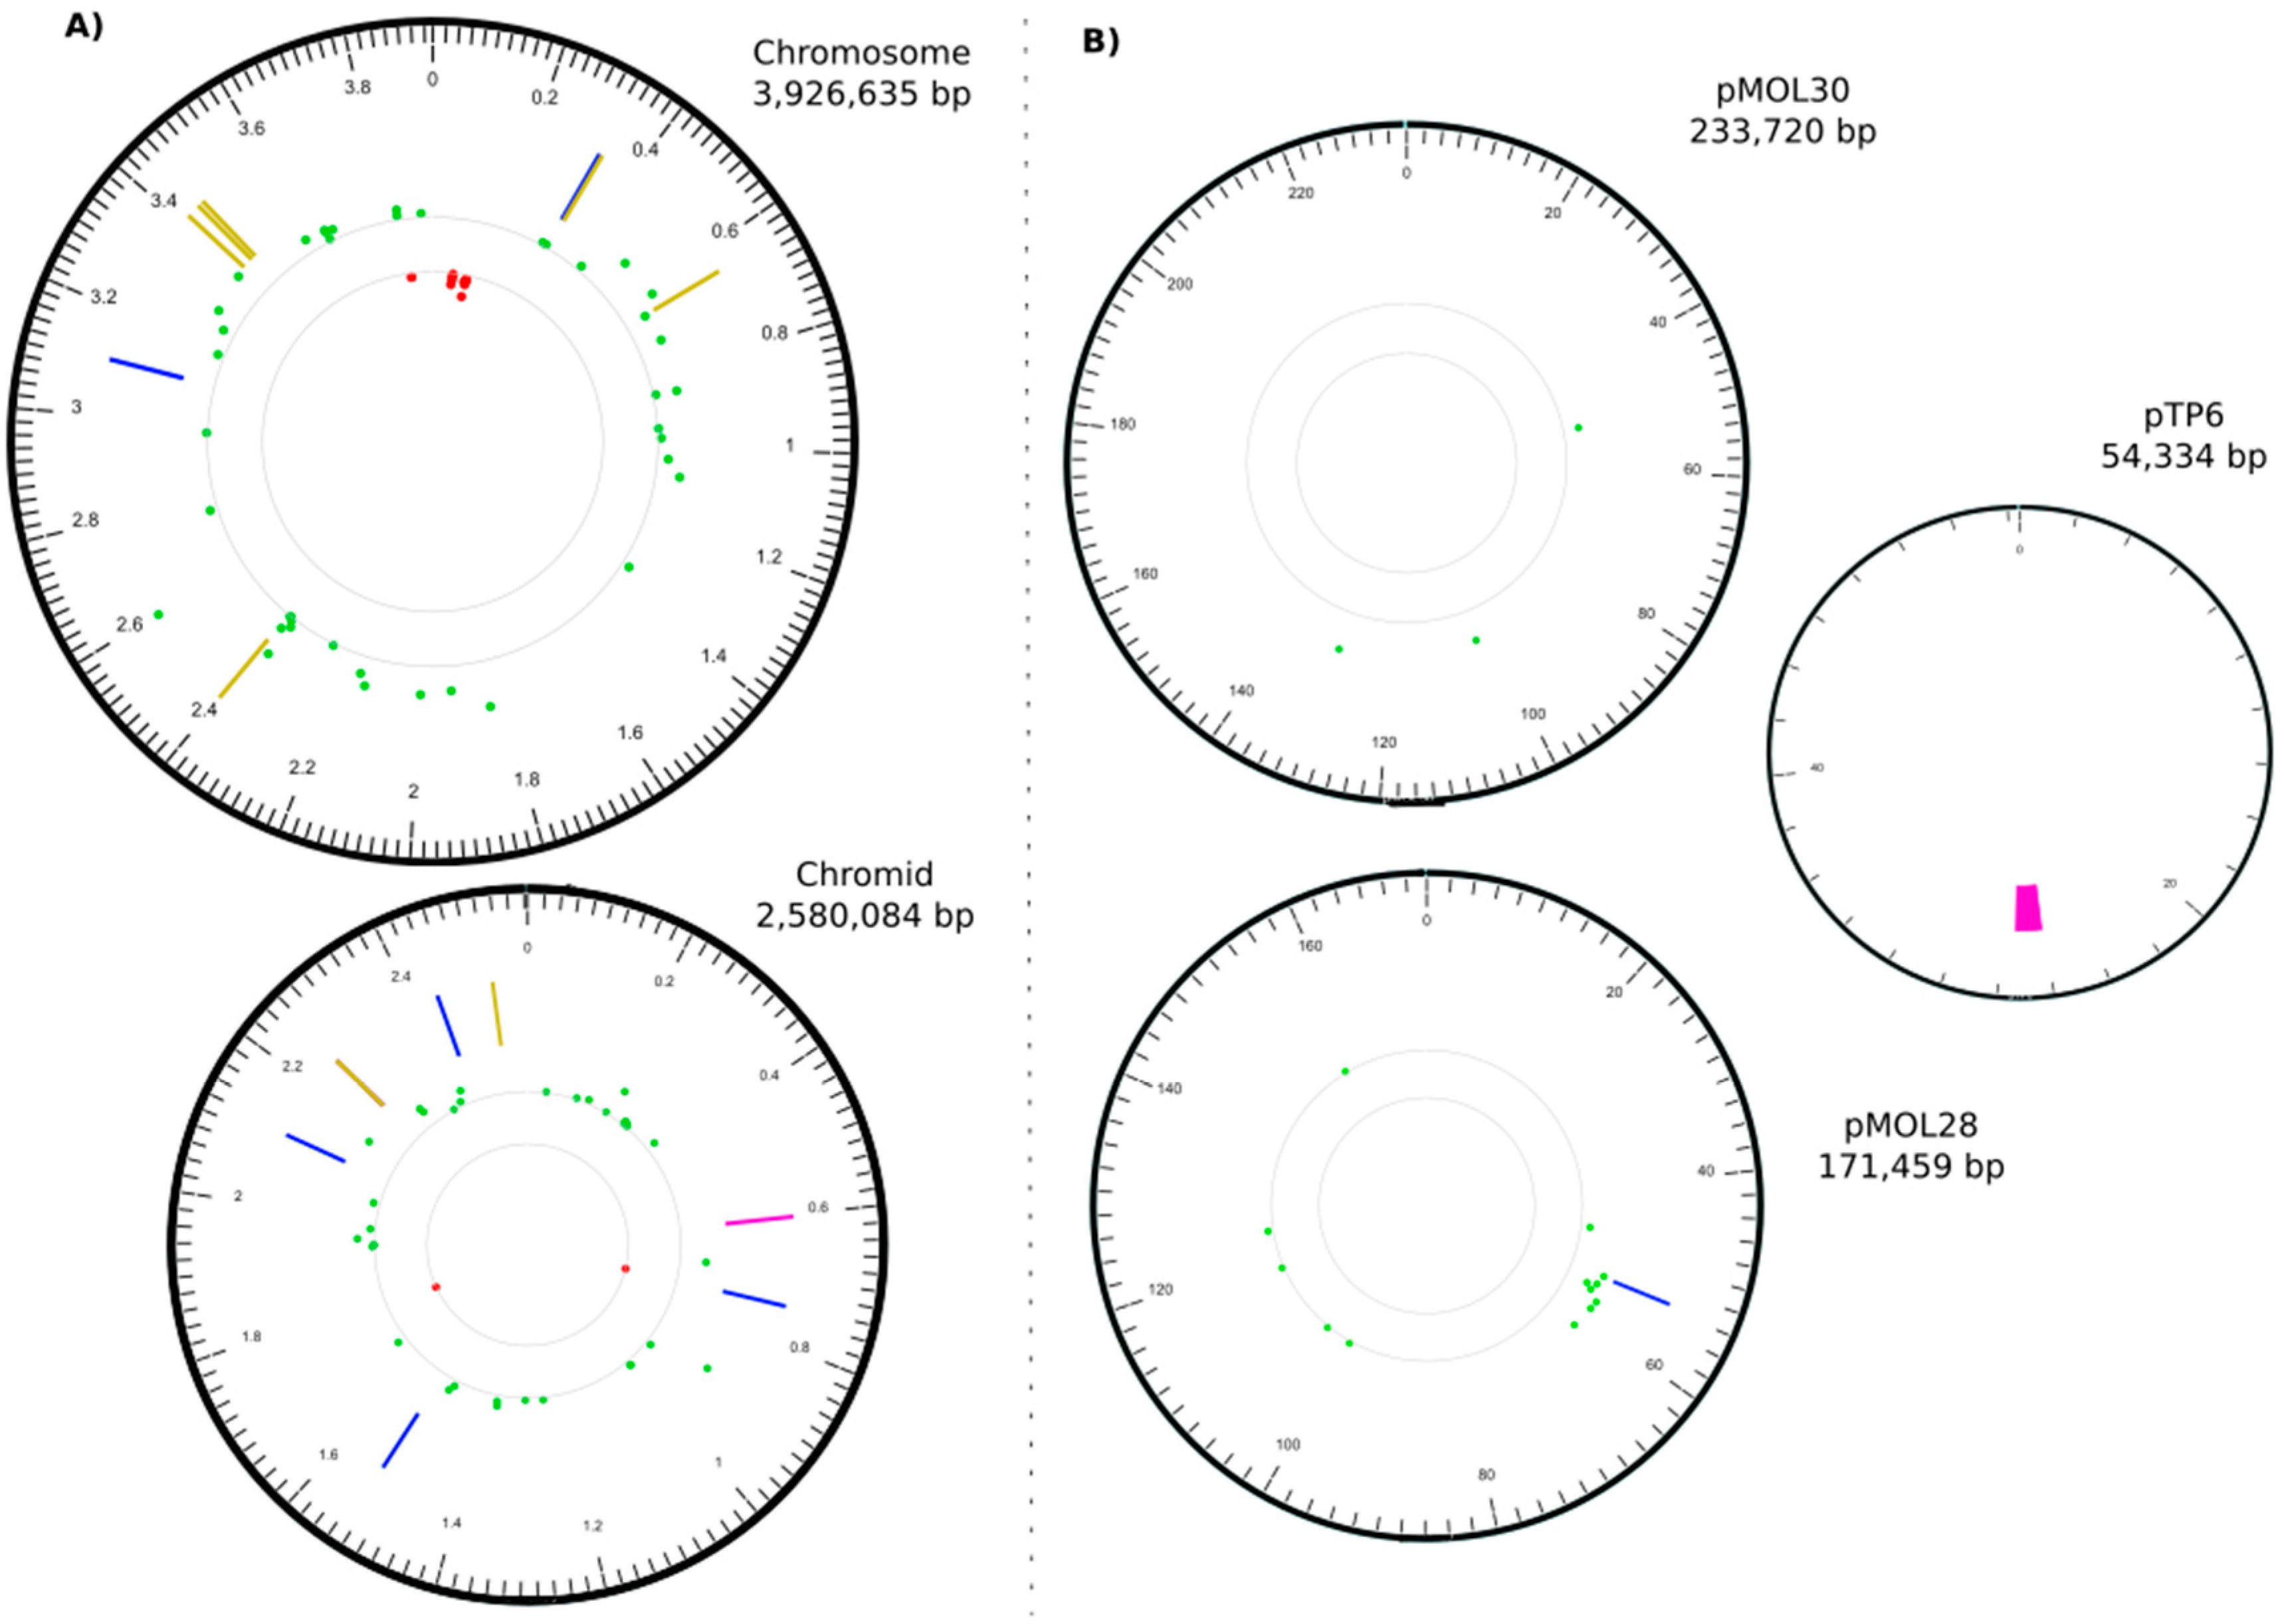
\includegraphics[width=\linewidth]{chapter3/chapter/figs/genes-09-00551-g001.png}
\end{center}
%\captionsetup{labelformat=empty}
\caption{Correlation map between Insertions or Deletions (INDELs), Single nucleotide polymorphisms (SNPs), and transcriptional changes found for \textit{C. metallidurans} MSR33. Concentric circles (ring) displayed from the outside inwards: (A) In ring 1, chromosome and chromid size scale in megabases (Mb) using a 20 kilobase (kb) window; (B) plasmids size scale in kb using a 2 kb window. In ring 2, position of insertion (blue), deletion (pink), and SNPs (mustard). INDELs and SNPs listed in Table \ref{table:42} and Table \ref{table:43}. In ring 3, each dot represents a single gene basal expression, overexpression (log$_2$ ratio $>$ 1, green), or repression (log$_2$ ratio $<$ -1, red), with a p-value $<$ 0.05. Circos plot created with Circa (http://omgenomics.com/circa).}
\label{chapter3-fig1}%
\end{figure*}


\begin{sidewaystable}
%\begin{table}[ht]
%\captionsetup{labelformat=empty}
\caption{Insertions (INs) and deletions (DELs) present in the genome of \textit{C. metallidurans} MSR33.\\}
\label{table:42}%
{%\hspace*{-4cm}
\begin{tabular*}{\columnwidth}{@{}llllllll@{}}
\hline
\textbf{Type} & \textbf{Replicon $^\#$} & \textbf{Start} & \textbf{End} & \textbf{Size (bp)} & \textbf{Description} & \textbf{Targeted} & \textbf{Function $^*$} \\
&  &  &  &  &  &  \textbf{Gene(s)}& \textbf{(MaGe Annotation)} \\
\hline
\\
IN & CHR1 &	328395 & 328395 & 1102 & IS1088 & Rmet\_0312 & Putative transporter \\
IN	& CHR1 & 3106728 & 3106728 & 1102 & IS1088 & Rmet\_2857 & Taurine ABC transporter \\
	&  &  &  &  &  &  (\textit{tauB}) &  ATP-binding protein\\
DEL &	CHR2 &	602035 &	602490 &	455	& &	Rmet\_4033 &	LysR family  \\
 &	 &	 &	 &		& &	& transcriptional regulator\\
IN &	CHR2 &	741818 &	741818 &	1102 &	IS1088 &	Rmet\_4160  &	EPS biosynthesis, \\
 &	 &	& &	 &	 & (\textit{pelF}) &	biofilm formation\\
IN &	CHR2 &	1529231 &	1529231 &	1102 &	IS1088 &	Rmet\_4867  &	Membrane fusion protein,\\
 &	 &	 &	 &	 &	 & (\textit{acrA}) &	multidrug efflux\\
IN &	CHR2 &	2113815 &	2113815 &	256 &	tniA/Tn3 &	Rmet\_5388  &	ApbE-like lipoprotein\\
 &	 &	 &	 &	 &	 &  (\textit{apbE}) & \\
IN &	CHR2 &	2253560 &	2253560 &	3 &	+CTT &	Rmet\_5508 &	Long-chain-fatty-acid\\
 &	 &	 &	 &	 & & & -CoA ligase\\
DEL &	CHR2 &	2253566 &	2253568 &	3 &	-CGG &	Rmet\_5508 &	Long-chain-fatty-acid\\
 &	 &	 &	 &	 & & & -CoA ligase\\
IN &	CHR2 &	2440975 &	2440975 &	1104 &	IS1088 &	Rmet\_5682 &	Membrane fusion protein, \\
 &	 &	 &	 &	 &	 &  (\textit{nimB})	& heavy metal transport\\
IN &	pMOL28 &	53484 &	53484 &	1104 &	IS1088 &	Rmet\_6205 &	Antisigma factor\\
DEL &	pTP6 &	26155 &	27385 &	1230 &	&	 (\textit{cnrY}),  &	Respectively an outer  \\
 &	 &	 &	 &	 &	& \textit{upf30.5}, & membrane protein, a \\
  &	 &	 &	 &	 &	& \textit{upf31.0}, &	DNA methylase, and \\
    &	 &	 &	 &	 &	& \textit{parA} &	a plasmid partition protein\\

\\
\hline
\hline
\end{tabular*}
} {\footnotesize{$^\#$ Chromosome: CHR1; chromid: CHR2. * Genomic and Metabolics analysis software (www.genoscope.cns.fr).} }
%\end{table}
\end{sidewaystable}

\begin{sidewaystable}
%\begin{table}[ht]
%\captionsetup{labelformat=empty}
\caption{ Single nucleotide polymorphisms (SNPs) detected in the genome of \textit{C. metallidurans} MSR33.\\}
\label{table:43}%
{%\hspace*{-4cm}
\begin{tabular*}{\columnwidth}{@{}llllll@{}}
\hline
\textbf{Replicon$^\#$} & \textbf{Position} & \textbf{SNP} & \textbf{SNP Type} & \textbf{Affected Gene} & \textbf{Gene Description$^*$} \\
\hline
CHR1 &	333850 & A→G & intergenic (+201/-75) &	Rmet\_0314 →/	& Putative transporter, major facilitator \\
 &	 &  &  & → \textit{ssb1}	& family/single-stranded DNA-binding \\
 &	 &  &  &	& protein (helix-destabilizing protein) \\
CHR1 &	645608	& A→G & A23A (GCA→GCG) &	Rmet\_0598  & Protein phosphatase family protein \\
 &	 &  &  & →	Ser/Thr	& \\
CHR1 &	2400725	& G→A	& intergenic (-77/+116) &	\textit{greA} ←/← \textit{carB} &	Transcription elongation factor/\\
&	 &  &  &	& carbamoyl-phosphate synthase large  \\
&	 &  &  &	& subunit  \\
CHR1 &	3418147	& A→G &	V295A (GTC→GCC) &	\textit{dppF} ←	& Dipeptide transporter; ATP-binding  \\
&	 &  &  &	& component of ABC superfamily \\
CHR1 &	3444412	& A→G &	V17A (GTC→GCC) &	\textit{nirJ} ← &	Heme d1 biosynthesis protein \\
CHR1 &	3456113 & A→G &	V76A (GTG→GCG) &	\textit{acyP} ← &	Acylphosphatase \\
CHR2 &	2253543 & A→T	& V158E (GTG→GAG) &	Rmet\_5508 ← &	Long-chain-fatty-acid-CoA ligase \\
CHR2 &	2253553 &	G→T	& P155T (CCG→ACG) &	Rmet\_5508 ← &	Long-chain-fatty-acid-CoA ligase \\
CHR2 &	2529357	& T→C &	G264G (GGA→GGG) & 	Rmet\_5769 ← & Esterase \\

\\
\hline
\hline
\end{tabular*}
} {\footnotesize{$^\#$ Chromosome: CHR1; chromid: CHR2; arrows show positive → or negative ← gene orientation; * www.genoscope.cns.fr.} }
%\end{table}
\end{sidewaystable}
The majority of the new IS1088 copies in the MSR33 genome were located on the chromosome and chromid, where all IS1088 copies indigenous to CH34 resided, but one IS1088 copy transposed into the \textit{cnrY} gene (Rmet\_6205) of pMOL28 (Table \ref{table:42}). This gene was part of the \textit{cnrYXHCBAT} locus involved in the inducible cobalt and nickel resistance in strain CH34, and encoded the anti-sigma factor CnrY that tethered, in conjunction with the sensor protein CnrX, the sigma factor CnrH, but released it in the presence of Ni$^{2+}$ or Co$^{2+}$ \citep{grass2000regulation, tibazarwa2000regulation}. The sigma factor CnrH promoted transcription of its own locus \textit{cnrYXH}, but also of the structural locus \textit{cnrCBA}, encoding a resistance nodulation division (RND)-driven efflux system \citep{janssen2010complete, kim2011switch}. The inactivation of the \textit{cnrY} gene in MSR33 by IS1088 inevitably led to the constitutive derepression of \textit{cnrCBAT} transcription and explained the increased cobalt and nickel resistance we observed for MSR33 (Table \ref{table:41}) (see also gene expression results in Section 3.3). A similar phenomenon was previously seen for spontaneous mutants of a pMOL30-less CH34 derivative, strain AE126 \citep{mergeay1985alcaligenes}, which showed a significantly increased resistance to cobalt and nickel \citep{collard1993new} and which was later acknowledged as being an IS- and frameshift-mediated inactivation of \textit{cnrY} and \textit{cnrX} \citep{vandecraen2016zinc}.
The other five genes affected by the insertion of an IS1088 element were Rmet\_0312 (\textit{nptA}) and Rmet\_2860 (\textit{tauB}), lying on the chromosome; and Rmet\_4160 (\textit{pelF}), Rmet\_4867 (\textit{acrA}), and Rmet\_5682 (\textit{nimB}), lying on the chromid (Table \ref{table:42}). The first three genes encode proteins with general cellular functions, and their inactivation is very unlikely to affect heavy metal resistance in strain MSR33. The fourth gene, \textit{acrA}, encodes a membrane fusion protein and is part of an intact \textit{acrABC} operon whose gene products form a tripartite multidrug efflux system. The last gene, \textit{nimB}, is involved in efflux-mediated heavy metal resistance, encoding also a membrane fusion protein resembling other membrane metal-binding fusion proteins in structure and function (e.g., CzcB, CnrB, CusB, and ZneB) by forming a periplasmic bridge between the cytoplasmic porter and the outer membrane channel \citep{kim2011switch}. Nonetheless, taking also into account that the \textit{nimA} gene is already inactivated in strain CH34 (and MSR33) by the presence of the insertion sequence element ISRme3 \citep{janssen2010complete}, it is hard to see how the inactivation of \textit{nimB} would result in the increased metal resistance we observed in strain MSR33. Two insertions were not attributed to IS1088. One appeared to be the result of a Tn3-related transposition event affecting gene Rmet\_5388, encoding a tentative ApbE-like lipoprotein, while the other concerned an unknown mutational event in gene Rmet\_5508 resulting in the insertion of a nucleotide triplet (+CTT) (Table \ref{table:42}). This gene encodes a long-chain fatty-acid CoA-ligase and also underwent a triplet deletion (-CGG) just a few nucleotides downstream of the triplet insert. As a combined result, the actual change at the protein level remained perfectly in-frame and gave a protein of the same length, but led to an altered peptide sequence at positions 149–153 (i.e., Xxx-Leu-Arg-Phe-Ala-Gln-Xxx in CH34 to Xxx-Leu-Phe-Ala-Lys-Gln-Xxx in MSR33 (amino acidic sequence change from Arg-Phe-Ala to Phe-Ala-Lys). The third deletion in MSR33 occurred in plasmid pTP6, effectively destroying the genes \textit{upf30.5}, \textit{upf31.0}, and \textit{parA}, immediately preceding Tn50580. Except for \textit{cnrY} and \textit{nimB}, none of the aforementioned genes are in any way associated with metal resistance.
In addition to the eight insertions and three deletions in the MSR33 genome, sequence analysis revealed the presence of nine single nucleotide polymorphisms (Table \ref{table:43}). Two of those occurred in intergenic regions on the chromosome, without apparent disruption of gene regulatory elements, while the other seven occurred in protein-encoding genes (four on the chromosome and three on the chromid). Except for the “silent” mutation (i.e., no \textit{aa} change) at position 645608, these Single nucleotide polymorphisms (SNPs) caused \textit{aa} substitutions in the corresponding gene products (Table \ref{table:43}). No SNPs were detected in any of the plasmids. Remarkably, gene Rmet\_5508 lying on the chromid (CHR2) once again was a target for mutation, displaying two SNPs in the immediate vicinity of the aforementioned triplet insertion and deletion in this gene (Table 3), bringing the full change of this region from RFAQKPAYV to FAKQKTAYE (changes are in bold and underlined). It is uncertain whether these protein changes would have any effect on the cellular and metabolic functions in MSR33.
Taken together, of the 11 Insertions or Deletions (INDELs) and nine SNPs identified by the whole genome resequencing of the \textit{C. metallidurans} strain MSR33, only the \textit{cnrY} inactivation by IS1088 and the concomitant derepression of \textit{cnrB} (see above) may be directly linked to the observed augmented heavy metal resistance in this strain, at least for Co$^{2+}$ and Ni$^{2+}$ (see above). None of the other genomic changes seemed to play a role in this augmentation. The augmented resistance for Cd$^{2+}$ in strain MSR33 (Table \ref{table:41}), however, remains a puzzle. The fact that such augmentation for Cd$^{2+}$ was only noted for MSR33 with an altered genome (i.e., with 17 INDELs and six SNPs), but not in CH34 transformed with plasmid pBBR::\textit{merTPAGB1} (Table \ref{table:41}) strongly indicates that the MSR33 genetic background was at play. In basic terms, bacterial resistance to toxic metals depends on two cellular processes, metal binding and metal transport, with the former generally being an intrinsic part of the latter. It is well established that many proteins or peptides that mediate the transport, buffering, or detoxification of metal ions in living cells have metal-binding domains (MBDs) in which certain amino acid residues (e.g., cysteine), as well as their structural layout and relative position to each other, play a key role in metal selectivity and specificity \citep{zheng2008data, thilakaraj2007silico}. While some of these proteins might be highly metal-specific, other proteins follow a more relaxed, nonspecific mode of metal binding. For instance, divalent metal uptake in \textit{C. metallidurans} is governed by a battery of redundant transporters that display a minimal degree of metal cation selectivity \citep{kirsten2011contributions}. Depending on the environment, this may lead to a cytoplasmic pool of unsolicited metal ions that at some point, particularly when reaching a toxic threshold, need to be removed by the cell. In \textit{C. metallidurans} this was done by one of three efflux systems: Cation diffusion facilitators (CDF), P-type ATPases, and the earlier mentioned RND-driven transenvelope transporters (HME-RND). Their main task in \textit{C. metallidurans}, because of this bacterium’s adaptation to metal-rich environments, was to balance the cytoplasmic and periplasmic concentrations of unwanted transition metals by entering the cellular arena and going into competition for metal cations with the “frivolous” metal uptake systems. Interestingly, all three types of metal efflux systems seemed to possess some degree of frivolity toward metal ions as well, albeit perhaps not as outspoken as for the metal uptake systems. The \textit{C. metallidurans} CzcD exporter (Rmet\_5979), for instance, allowed as a CDF protein Zn$^{2+}$, Cd$^{2+}$, or Co$^{2+}$ as a substrate \citep{anton1999czcd}, whereas the DmeF and FieF exporters (Rmet\_0198 and Rmet\_3406) displayed as CDF family members broad metal specificity for Zn$^{2+}$, Cd$^{2+}$, Co$^{2+}$, and Ni$^{2+}$ \citep{munkelt2004chromosomally}. It is worth mentioning that disruption of the \textit{dmeF} gene in strain CH34 dramatically lowered the resistance for Co$^{2+}$ (but not for Zn$^{2+}$, Cd$^{2+}$, and Ni$^{2+}$), indicating a complex interplay between the DmeF exporter and the CzcCBA and CnrCBA efflux pumps (possibly partially obscured by the action of other metal resistance systems) \citep{munkelt2004chromosomally}. Moreover, CDF proteins can play diverse roles and may possess different metal ion selectivity depending on the environmental conditions (i.e., by adjusted Kd values for certain metals) \citep{barber2017transition}. In addition, the eight metal resistance-related P1B-type ATPases currently identified in strain CH34 can be subdivided into two groups according to their substrate profile \citep{nies2016biological}: Those that extrude Cu$^+$ and Ag$^+$ (CupA and CupF) and those that extrude Zn$^{2+}$, Cd$^{2+}$, Co$^{2+}$, or Pb$^{2+}$ (ZntA, CadA, PbrA, and CzcP). These exporters mainly differ in the presence of unique amino acid sequences in their transmembrane MBDs, hence defining their metal specificity. But even within a subgroup, differences may exist in terms of metal affinity. For example, CzcP encoded by plasmid pMOL30 is unable to mediate Zn resistance on its own but rather augments the metal exportability of the ZntA, CadA, and PbrA exporters \citep{scherer2009czcp}. In a similar fashion, the five active HME-RND efflux systems in strain CH34 displayed a limited substrate spectrum, pumping out either the monovalent metal cations Cu$^+$ and Ag$^+$ (CusA, SilA) or the divalent metal cations Zn$^{2+}$, Ni$^{2+}$, and Co$^{2+}$, with occasionally also Cd$^{2+}$ (ZniA, CnrA, CzcA) \citep{nies2016biological} (Figure \ref{chapter3-fig2}). In such HME-RND systems, two steps of heavy-metal extrusion were discerned, the periplasmic and the transenvelope efflux (Figure \ref{chapter3-fig2}). Each step involved the interaction of metals with MBDs within the Membrane Fusion Protein (MFP) and RND proteins. Sometimes, the delivery of periplasmic metal ions to the typical C3B6A3-complex is facilitated by a small periplasmic metallochaperone, as is the case for the \textit{E. coli} CusCBFA system \citep{delmar2014bacterial} (and likely, based on CusF \textit{aa} sequence similarities, also the CusCBAF complex of strain CH34). Little is known about the substrate specificity of the metal-binding proteins of HME-RND efflux complexes. Apparently, metal-induced conformational changes in the C3B6A3-complex are required in order to create a proper metal-guiding C3B6A3 channel for metal export to take place \citep{kim2011switch,de2010metal,long2012structure,pak2013structures}.

\begin{figure*} [ht] 
\begin{center}
%\hspace*{-2.5cm}
\begin{subfigure}{0.48\textwidth}
    %\caption{Extracts and \textit{in vitro} experiment setup}
    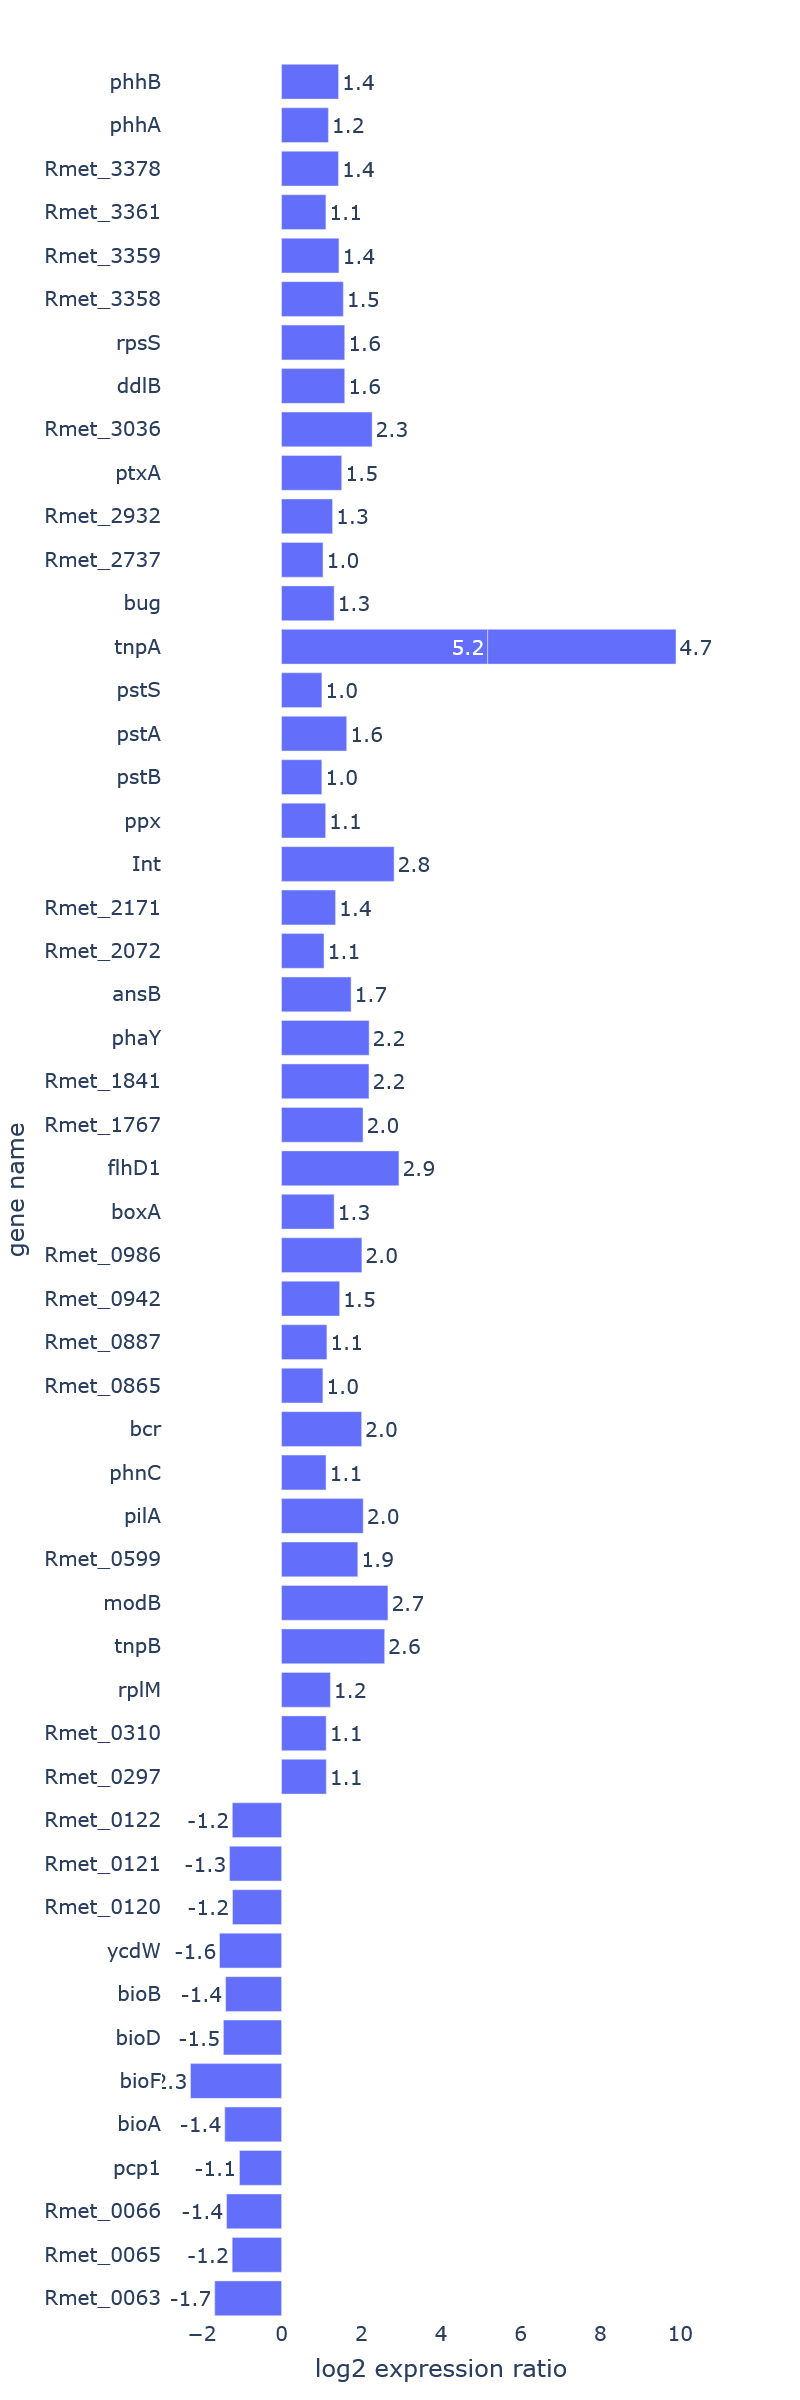
\includegraphics[width=\linewidth]{chapter3/chapter/figs/newplot(8).png}
     \label{fig:4a}
  \end{subfigure}
   \begin{subfigure}{0.48\textwidth}
    %\caption{Mytilid neutral red alive stain }
    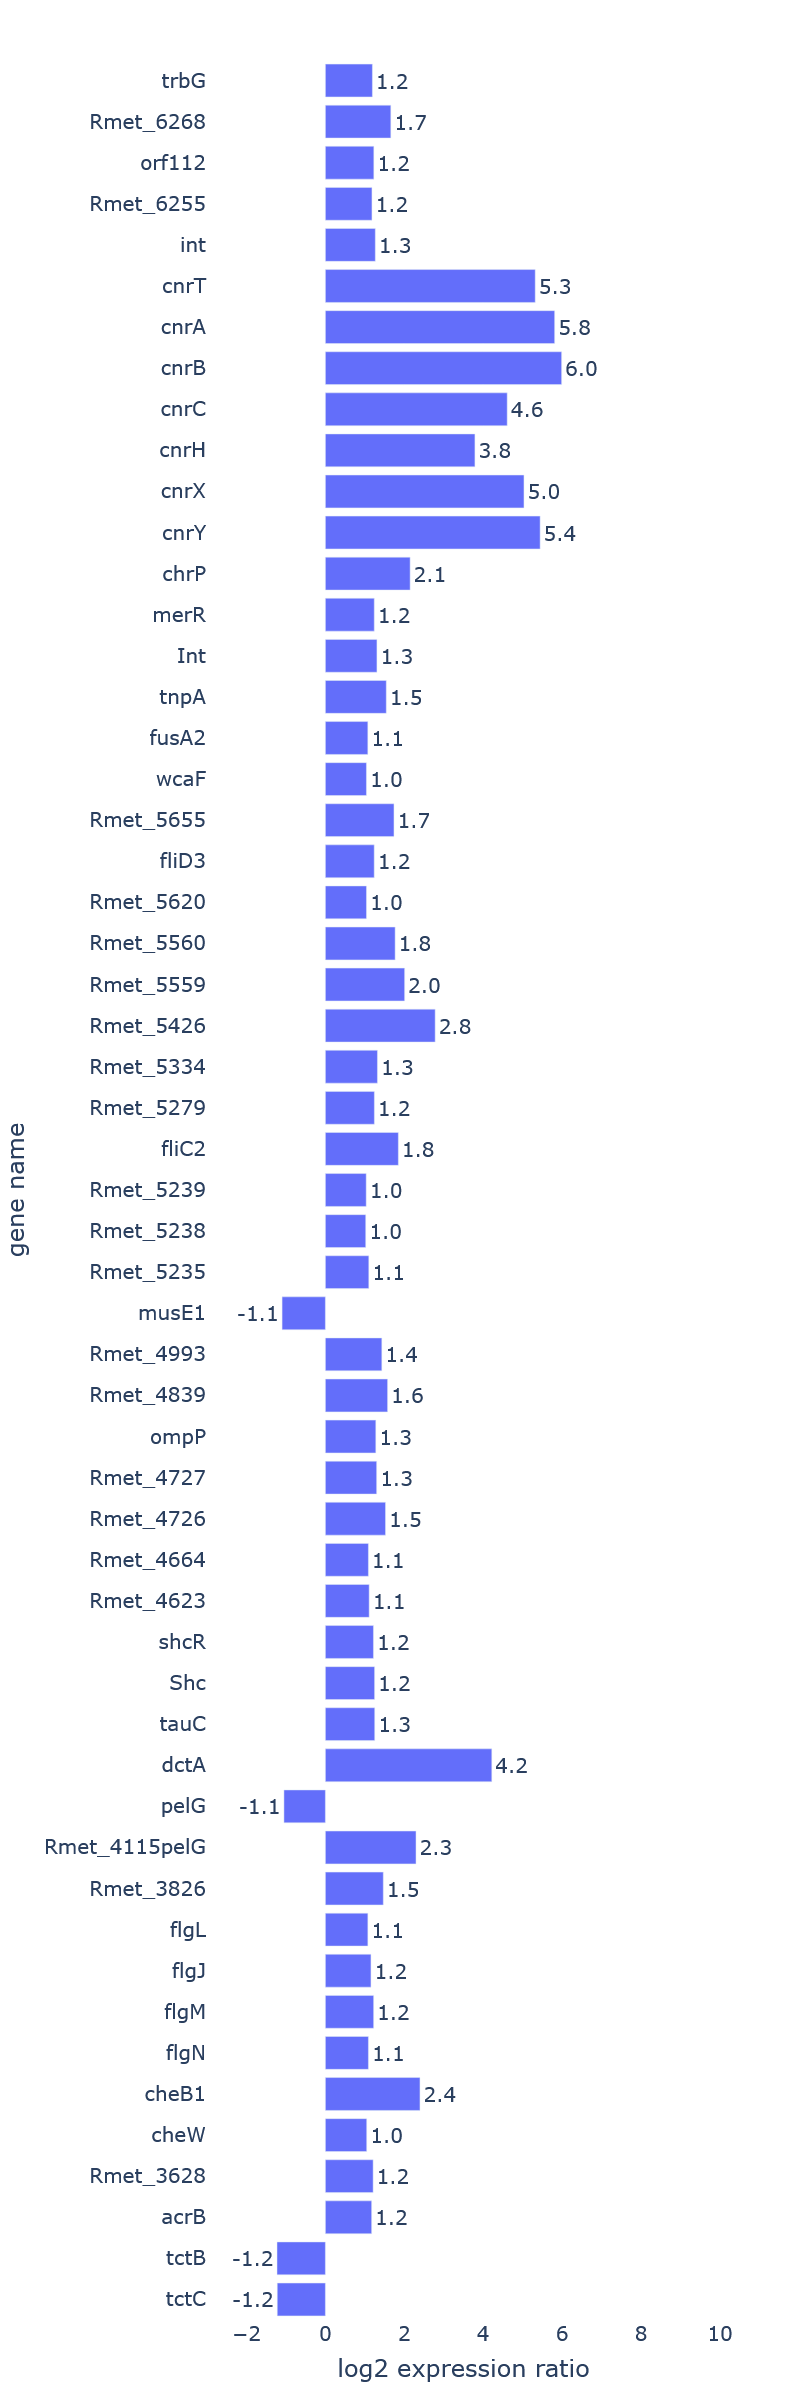
\includegraphics[width=\linewidth]{chapter3/chapter/figs/newplot(7).png}
     \label{fig:4b}
  \end{subfigure}
\end{center}
%\captionsetup{labelformat=empty}
\caption{Transcriptional changes in\textit{ C. metallidurans} MSR33 with respect to CH34, with both strains grown under equal and non-selective conditions (see methods). Bar graphs show the significantly (p-value $<$ 0.05) higher expression (log$_2$ ratio $>$ +1) and lower expression (log$_2$ ratio $<$ -1) of MSR33 genes (with CH34 gene expression levels as reference). 
}
\label{chapter3-fig2}%
\end{figure*}

\begin{figure*} [ht] 
\begin{center}
%\hspace*{-2.5cm}
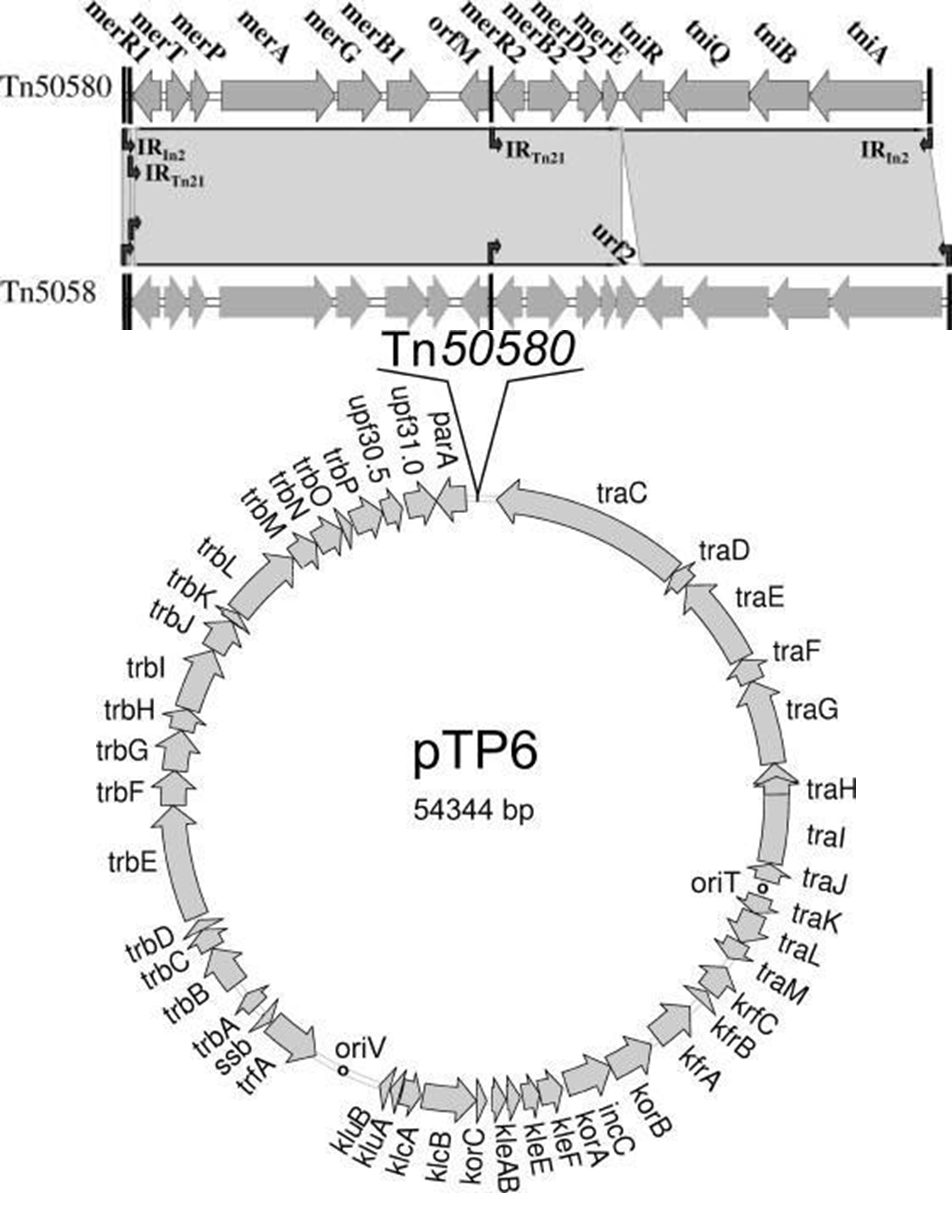
\includegraphics[width=300px]{chapter3/chapter/figs/genes-09-00551-g003.png}
\end{center}
%\captionsetup{labelformat=empty}
\caption{Genetic map of plasmid pTP6. Figure adapted from Smalla \textit{et al.}, 2006 (Copyright\textsuperscript{\tiny\textcopyright} 2006, Appl Environ Microbiol. 2006 Nov; 72(11): 7253–7259).   
}
\label{chapter3-fig3}%
\end{figure*}


As mentioned, it is not inconceivable that the genetic changes in MSR33 instigated cellular conditions or pleiotropic effects that were generally favourable for Cd$^{2+}$ detoxification and hence led to the observed improvement in Cd$^{2+}$ resistance. Possibly, this involved the temporal recruitment of one or more metal binding export proteins, from known metal resistant systems or from hitherto unknown export systems, able to bind Cd$^{2+}$. The transition metals cadmium and mercury belong to Group 12 of chemical elements in the periodic table, together with zinc and copernicium. Although these four metals differ in significant respects, they also have common properties. Particularly, Cd and Hg are similar in their outer shell electron configuration (d$^{10}$s$^2$) and atomic radius (ca. 150 pm), and their cations both have a high affinity for sulfhydryl groups in cellular compounds and proteins (i.e., in methionine and cysteine residues). From this perspective, competition between Cd$^{2+}$ and Hg$^{2+}$ for certain MBDs cannot be excluded. Bacterial evolution and adaptation to new or rapidly changing environments implies a delicate balance between the safeguarding of genome integrity and the tolerance for genome instability. A too-rigid genome inevitably will lead to the demise of innovative power and hence adaptability of the host, whereas a too plastic or “fluid” genome may lead to disadvantageous mutations and cell growth arrest, or even cell death. This balance between beneficiary and perilous change in a bacterial genome also relates to the general fitness and the energy household of its host. Members of the genus \textit{Cupriavidus}, and in particular \textit{C. metallidurans}, appear to be masters in adaptation as they are home to a wide variety of habitats, often in extreme conditions \citep{sota2007region,leys2009response,mijnendonckx2013characterization,byloos2017impact}. The introduction of the 54 kb plasmid pTP6 into a strain already carrying two large replicons of 3.9 and 2.6 Mb (chromosome and chromid, respectively) and two megasized plasmids of 171 and 234 kb (pMOL28 and pMOL30, respectively) could be seen as a serious additional burden to the host regardless of whether or not phenotypical or physiological changes occur.
Because the charting of genomic changes in MSR33 with respect to its parental strain CH34 did not provide us with any clues or direct evidence on the involvement of certain genetic loci or of any of the known metal resistance determinants on the observed augmented Cd$^{2+}$ resistance, we decided to compare the basal gene expression data for strains CH34 and MSR33 using RNA microarray technology in an attempt to associate their gene expression profiles with strain-specific physiological behaviour, with a focus on differentially expressed (DE) genes that might be involved in the cellular detoxification of heavy metals such as Cd$^{2+}$.

\subsection{Transcriptional Analysis of Strain MSR33}

Strains CH34 and MSR33, which were equally grown in nonselective conditions without any metal-related stress, were investigated for basal gene expression levels, and their expression profiles were compared. A total of 107 DE genes showed statistically significant changes in their expression (Figure \ref{chapter3-fig2}). Affected genes pertained to the main chromosome (55 genes), the chromid (36 genes), and the plasmids pMOL30 (3 genes) and pMOL28 (13 genes) (Figure \ref{chapter3-fig2}). In general terms, the products of these 107 genes could be grouped according to their predicted annotated function \citep{janssen2010complete}: Catalytic function (35 genes), transport (24 genes), transcriptional regulation (11 genes), recombination (6 genes), movement and chemotaxis (9 genes), and miscellaneous (22 genes). Most of these genes had a higher expression in strain MSR33, with only 16 genes in strain MSR33 showing a lower expression level. What is immediately striking is that all genes of the \textit{cnrYXHCBAT} operon on plasmid pMOL28 had a significantly higher expression (Figure \ref{chapter3-fig2}), with log$_2$ fold changes ranging from four to six. As we know from MSR33 whole genome sequence analysis, this high expression of the \textit{cnr} locus in strain MSR33 was the direct result of IS1088-mediated \textit{cnrY} inactivation and hence derepression of the \textit{cnr} locus, explaining the increased resistance we observed for strain MSR33 to Co$^{2+}$ and Ni$^{2+}$ (see previous sections). Equally noticeable is the complete absence of an altered expression of the \textit{czc} locus on pMOL30, strongly suggesting that the augmented Cd$^{+2}$ resistance we see for strain MSR33 was independent of this locus. This, in fact, corroborates earlier findings about the pMOL30-less CH34 derivative AE126 (which, like MSR33, also has an IS1088-mediated inactivated \textit{cnrY} gene on the remaining plasmid pMOL28):  \citet{vandecraen2016zinc} showed, next to a heightened resistance to Zn$^{2+}$, Co$^{2+}$, and Ni$^{2+}$, a 2-fold increased resistance to Cd$^{2+}$. Adding another level of complexity, when strains AE126 and AE104 (a CH34 derivative lacking both pMOL28 and pMOL30 plasmids \citep{mergeay1985alcaligenes}) were transformed with pTP6, these strains, like MSR33, gained an improvement in Cd$^{2+}$ resistance, albeit to a lesser extent (Rojas LA, personal communication).
This would indicate that the augmentation of Cd$^{2+}$ resistance in MSR33 by pTP6 conjugation should be seen as a layered process brought about by multiple factors and possibly diverse mechanisms supporting each other. We cannot say at this point what these mechanisms precisely are and how and when they are triggered, as we have no information about the genomic changes in pTP6 conjugants of AE104 and AE126 (as pTP6 conjugation in CH34 causes genomic changes, this would most likely also be the case for pTP6 conjugation in strains AE104 and AE126, but not necessarily involving the same genomic changes). Clearly, further studies are needed to understand the augmented metal resistance in pTP6 conjugants of CH34 and its derivatives, including (1) the resequencing of pTP6-conjugated AE104 and AE126 strains and (2) the extensive RNAseq-based genetic response analyses for a wider range of heavy metals in all three pTP6-conjugated strains. The additional possibility that some of the observed genetic changes were already introduced to the recipient CH34 strain prior to conjugation with pTP6 cannot be entirely excluded. Lastly, the plasmid-curing procedures used to obtain strains AE104 and AE126 (i.e., applying mitomycin C, nalidixic acid, or hydroxyurea to growing CH34 cells \citep{mergeay1985alcaligenes}) may also have had mutagenic effects or may have induced transposition activity. In this respect, it would be best, in the frame of future studies, to resequence these strains as well.
A very high log$_2$ fold difference in the expression of $>$4 was also noted in strain MSR33 for the Rmet\_4229 gene, a \textit{dctA} paralogue whose product was functionally annotated as a C4-dicarboxylate transporter and which is unlikely to have any connection to metal detoxification or resistance, and gene Rmet\_2382, originally identified in CH34 as a transposase-encoding \textit{tnpA} gene (IS1088) (Figure \ref{chapter3-fig2}). Intermediate high log$_2$ fold changes of $>$2 were seen in strain MSR33 for another 17 genes, whereas the remaining 72 genes showed a log$_2$ fold change between one and two. None of these genes is thought to be involved in metal binding, metal detoxification, or metal resistance. Among the genes with lowered expression in strain MSR33, we noted the \textit{pelG} gene (Rmet\_4161), which is part of the \textit{pelABCDEFG} operon required to produce an extracellular polysaccharide that has been implicated in biofilm development \citep{vasseur2005pel}. Our sequence data confirmed that the IS1088 element transposed into the \textit{pelF} gene (Table \ref{table:42}), thereby disrupting expression of the \textit{pelG} gene. This could explain the complete lack of biofilm formation in strain MSR33 reported to us by P. Alviz in a personal communication.
In conclusion, the genome of MSR33 underwent eight insertions, three deletions, and nine SNPs. At least seven of the insertions were due to the action of mobile genetic elements, with their presence fully confirmed by sequence data (implicating IS1088 in six cases), whereas one small insertion and all three deletions in strain MSR33 may have been the result of DNA recombination or transposition events. The \textit{C. metallidurans} genome is known to be ridden with a very high number of mobile genetic elements, with 57 IS elements, 19 other transposable elements, and 16 genomic islands for its type strain CH34 \citep{janssen2010complete,van2009new,van2012variation}. In concordance with this genomic fluidity, \textit{C. metallidurans} displays a highly versatile metabolism and an inherent ability to inhabit a variety of harsh environments \citep{sobecky2009horizontal,sota2007region,leys2009response,mijnendonckx2013characterization,byloos2017impact}. This adaptability has not come about overnight but is the wonderful result of microbial evolution over long periods of time. In a time in which large chunks of DNA were retrieved from the environment (e.g., by plasmid transfer or gene exchanges), adaptation was brought about by DNA mutations and natural selection and molecular inventions took place, steadily moulding the genome into its present large (6.9 Mb) and highly malleable form, providing the bacterium with a vast array of possibilities for rapid genetic responses (hence its well-chosen epithet as “Master Survivalist”) \citep{janssen2010complete}. However, tinkering with this hugely evolved and dynamic genome holds intrinsic dangers. Although the plasmid pTP6 was maintained stably in strain CH34 (i.e., MSR33) for over 70 generations under nonselective conditions \citep{rojas2011characterization}, it has now become clear from our study at hand that the receiving host’s genome underwent multiple changes in the form of 11 INDELs and 9 SNPs, affecting the physiology and heavy metal resistance of the host. It would be wrong to point the finger at the extra plasmid as the “usual suspect” for these genetic changes, but rather we hold the actual process of conjugation responsible. Conjugative interaction appears to be a strong stimulus for transposition \citep{godoy2000transposon,christie2009conjugative,baharoglu2010conjugative}, and hence it is easy to envisage that, as a result of conjugation procedures, some elements of the extensive mobilome of \textit{C. metallidurans} (with nearly 100 mobile elements) were triggered into action and “moved around”, causing genetic changes that led to clearly perceptible but also less visible (and less understood) effects alike. The take-home message here is that the genetic engineering of bacteria with large complex and dynamic genomes should be carried out with much caution and that a strong preference should be given to the new generation of small broad-host-range cloning vectors and CRISPR-based technologies nowadays available \citep{jain2013broad,obranic2013improvement,tian2017fundamental,cook2018genetic,xiong2018genome}.

\begin{figure*} [ht] 
\begin{center}
\hspace*{-1.5cm}
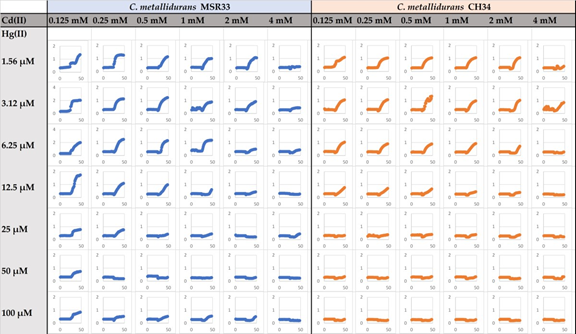
\includegraphics[width=500px]{chapter3/chapter/figs/genes-09-00551-g004.png}
\end{center}
%\captionsetup{labelformat=empty}
\caption{Effect of various mixtures of Hg$^{2+}$ and Cd$^{2+}$  on \textit{C. metallidurans} strains MSR33 and CH34 growth.   
}
\label{chapter3-fig4}%
\end{figure*}

\section{Supplementary Materials}

The following are available online at https://www.mdpi.com/2073-4425/9/11/551/s1. Figure S1: Genetic map of plasmid pTP6; Table \ref{table:44}: Primers designed for this report; Table \ref{table:45}: Transcriptional changes observed in MSR33 versus CH34 under basal conditions; Table \ref{table:46}: Homology analysis of \textit{mer} gene products present in plasmid pTP6; Figure \ref{chapter3-fig4}: Effect of various mixtures of Hg$^{2+}$ and Cd$^{2+}$ on \textit{C. metallidurans} strains MSR33 and CH34 growth; Table \ref{table:47}: Plasmid copy number (PCN) for \textit{C. metallidurans} strains MSR33 and CH34, determined by quantitative PCR; Table \ref{table:48}: mer gene occurrences on the replicons of strains CH34 and MSR33.

\section{Author Contributions}

F.A.M., P.J.J., R.V.H., P.M., and L.A.R. conceived and designed the experiments; F.A.M., A.J., and A.P. performed the experiments; F.A.M., R.V.H., and P.M. analyzed the data; L.A.R. and P.J.J. contributed reagents, materials, and analysis tools; F.A.M., P.J.J., R.V.H., P.M., and L.A.R. wrote the paper.
Funding
SCK$\cdot$CEN EE0630012-09 (to P.J.J., R.V.H., A.J., A.P., and P.M.), CONICYT/FONDECYT 11130117 (L.A.R.), and CONICYT/BC-PhD 72170403 (F.A.M.)

\section{Acknowledgments}
Authors acknowledge research funding by SCK$\cdot$CEN EE0630012-09 (to P.J.J., R.V.H., A.J., A.P., and P.M.), CONICYT/FONDECYT 11130117 (L.A.R.), and CONICYT/BC-PhD 72170403 (F.A.M.). Genome sequencing was provided by MicrobesNG (http://www.microbesng.uk), supported by BBSRC grant number BB/L024209/1. We thank D. Vallenet and Z. Rouy of Génoscope (Centre National de Séquençage, Evry, France) for implementing additional features in MaGe and their essential advice in genome annotation.

\section{Conflicts of Interest}
The authors declare no conflicts of interest. The founding sponsors had no role in the design of the study; in the collection, analyses, or interpretation of data; in the writing of the manuscript; or in the decision to publish the results.


\begin{sidewaystable}[ht]
%\captionsetup{labelformat=empty}
\caption{Primers used in this study.\\}
\label{table:44}%
{%\hspace*{-5cm}
\begin{tabular*}{\columnwidth}{@{}lllll@{}}
\hline
\textbf{Targeted gene} & \textbf{Replicon} & \textbf{Primer} & \textbf{Sequence (5'-3')} \\
\hline
\textit{merTPAGB1} & pTP6 & pTP6mer\_Fw & CACTATAGGGCGAATTACGGTCTTTTCTGACGTTGG\\
& & pTP6mer\_Rv & AAGGGAACAAAAGCTGTTCTAGCCACTTTCGGTTCG\\
MCS & pBBR1 & pBBR1MCS2\_GA\_Fw & CAGCTTTTGTTCCCTTTAGTGAG\\
 &  & pBBR1MCS2\_GA\_Rv & AATTCGCCCTATAGTGAGTCGTAT\\
\textit{cadA} & Chromosome & CadA\_Fw\_CR1 & GCACACTCACACATGGCAAG\\
 &  & CadA\_Rv\_CR1 & CTGAGACACAGGATGGTCCG\\
\textit{zniA} & Chromid  & ZniA\_Fw\_CR2 & GCGCAGATCACCCAGGAATA\\
 &  & ZniA\_Rv\_CR2 & ACTATGACCGTTCGACGCTG\\
\textit{nccA} & pMOL30 & NccA\_Fw\_P30 & AAGAGTGAATGGCCGGATGG\\
 &  & NccA\_Rv\_P30 & TCTCAATGGGTTGGGTGACG\\
 \textit{cnrA} & pMOL28 & CnrA\_Fw\_P30 & AAATGTCCCGATCACAGTCGG\\
 &  & CnrA\_Rv\_P30 & GCCCACCACCGTTTCATTG\\
  \textit{merG} & pTP6 & MerG\_Fw\_PT6 & TACAAATGCGGTATGGGCGT\\
 &  & pTP6\_Rv\_PT6 & CGAGGTTGAACTGTGCATCG\\
\\
\hline
\hline
\end{tabular*}
}
\\
{
%\footnotesize{}
}
\end{sidewaystable}


\begin{table}[ht]
%\captionsetup{labelformat=empty}
\caption{Transcriptional changes in MSR33 vs CH34 under equal, non-selective conditions.\\}
\label{table:45}%
{%\hspace*{-5cm}
\begin{tabular*}{\columnwidth}{@{}lll@{}}
\hline
 & \textbf{No genes} & \textbf{\%Total} \\
\hline
Total genes & 6099 & 100\\
Pval $>$0.05 & 5462 & 89.56\\
Pval $<$0.05 & 637 & 10.44\\
Overexpressed (log$_2$ $>$1) & 87 & 0.014\\
Repressed (log$_2$ $<$-1) & 15 & 0.002\\
Highly overexpressed (log$_2$ $>$2) & 27 & 0.004\\
Highly repressed (log$_2$ $<$-2) & 1 & 0.001\\
\\
\hline
\hline
\end{tabular*}
}
\\
{
%\footnotesize{}
}
\end{table}



\begin{sidewaystable}[ht]
%\captionsetup{labelformat=empty}
\caption{Sequence similarity of \textit{mer} gene products present in plasmid pTP6.\\}
\label{table:46}%
{%\hspace*{-5cm}
\begin{tabular*}{\columnwidth}{@{}lllll@{}}
\hline
 \textbf{Gene} & \textbf{Protein (aa)} & \textbf{Function} & \textbf{Organism (Reference)} & \textbf{\%ID (aa)}\\
 \hline
 \textit{merR1} & MerR (144) & activator/repressor of \textit{mer} operon & \textit{C. metallidurans} CH34 & 95\% (144) \\
  &  &  &  (YP\_145639.1) &  \\
 \textit{merT} & MerT (116) & mercuric ion transport protein & \textit{C. metallidurans} CH34  & 87\% (116) \\ 
   &  &  &  (YP\_145638.1) &  \\
 \textit{merP} & MerP (91) & periplasmic mercuric-ion binding protein & \textit{C. metallidurans} CH34  & 77\% (91) \\
    &  &  &  (YP\_145637.1) &  \\
 \textit{merA} & MerA (569) & mercuric-ion reductase Fad flavoprotein & \textit{C. metallidurans} CH34  & 71\% (561) \\ 
     &  &  &  (YP\_145636.1) &  \\
 \textit{merG}* & MerG (217) & organomercurial transporter & \textit{C. testosterone} JL40  & 100\% (190) \\ 
     &  &  &  (KGH30768.1) &  \\
 \textit{merB-}1* & MerB(212) & organomercurial lyase & \textit{B. cepacia} 2a  & 100\% (212) \\
    &  &  &  (YP\_006965881.1) &  \\
\textit{merR}2 & MerR (144) &
activator/repressor of \textit{mer} operon & \textit{C. metallidurans} CH34  & 93\% (144)\\
&&&(YP\_145639.1)&\\
\textit{merB}-2* & MerB (212) & organomercurial lyase & \textit{B. cepacia} 2a  & 100\% (212) \\
    &  &  &  (YP\_006965883.1) &  \\
\textit{merD} & MerD (121) & secondary regulatory protein & \textit{C. metallidurans} CH34  & 92\% (121) \\
    &  &  &   (YP\_145635.1) &  \\
\textit{merE} & MerE (78) & membrane mercuric resistance protein & \textit{C. metallidurans} CH34   & 79\% (78)\\
    &  &  &  (YP\_145634.1) &  \\
\\
\hline
\hline
\end{tabular*}
}
\\
{
\footnotesize{*Genes not present in \textit{C. metallidurans} CH34}
}
\end{sidewaystable}

\begin{sidewaystable}[ht]
%\captionsetup{labelformat=empty}
\caption{Plasmid copy number (PCN) for \textit{C. metallidurans} strains MSR33 and CH34.\\}
\label{table:47}%
{%\hspace*{-5cm}
\begin{tabular*}{\columnwidth}{@{}llllllllll@{}}
\hline
 \textbf{Replicon} & \textbf{Ct} & \textbf{SD} & \textbf{Log$_{10}$(DNA)} & \textbf{PCN}  & \textbf{Ct} & \textbf{SD} & \textbf{Log$_{10}$(DNA)} & \textbf{PCN} & \textbf{Average PCN}\\
 \hline
Chromosome (\textit{cadA}) & 23.38 & 0.05 & 10.18 & 1.00 & 23.47 & 0.21 & 10.18 & 1.00  & 1.00\\
Chromid (\textit{zniA}) & 20.90 & 0.19 & 10.24 & 1.16 & 20.18 & 0.07 & 10.24 & 1.14  & 1.15\\
pMOL30 (\textit{nccA}) & 21.71 & 0.29 & 10.26 & 1.21 & 19.75 & 0.20 & 10.24 & 1.14  & 1.18\\
pMOL28 (\textit{cnrA}) & 27.80 & 0.24 & 10.25 & 1.18 & 24.62 & 0.07 & 10.23 & 1.12  & 1.15\\
pTP6 (\textit{merG})* & 20.67 & 0.08 & 10.50 & 1.81 & 35.28 & 0.60 & 9.48 & 0.17  & 0.99\\
\\
\hline
\hline
\end{tabular*}
}
\\
{
\footnotesize{*Gene not present in \textit{C. metallidurans} CH34}
}
\end{sidewaystable}

\begin{table}[ht]
%\captionsetup{labelformat=empty}
\caption{\textit{mer} gene  occurrence  on  replicons  of  strains  CH34  and  MSR33  (individual  genes  of  the \textit{merRT}, \textit{merRTPA}, \textit{merRDE}, \textit{merRTPA} or \textit{merRTPADE} loci are indicated).\\}
\label{table:48}%
{%\hspace*{-5cm}
\begin{tabular*}{\columnwidth}{@{}llllllll@{}}
\hline
 \textbf{Replicon} & \multicolumn{6}{c}{\textbf{\textit{mer} genes present on each replicon }} & \textbf{PCN*} \\
 \hline
CHR1 & R & T & P & A &   &   & 1.00\\
pMOL28 & R & T & P & A & D & E & 1.15\\
pMOL30 - cluster 1 & R & T & P & A & D & E & 1.18\\
pMOL30 - cluster 2 & R & T & P & A & D & E & 1.18\\
Strain CH34 & 4.51 & 4.51 & 3.33 & 3.33 & 2.33 & 2.33 & \\
pTP6 - cluster 1 & R & T & P & A &  &  & 1.8\\
pTP6 - cluster 2 & R &  &  &  & D & E & 1.8\\
Strain MSR33 & 8.11 & 6.31 & 5.13 & 5.13 & 4.13 & 4.13 & \\
Gene unit increase & +2 & +1 & +1 & +1 & +1 & +1 & \\
Gene content increase & 80\% & 40\% & 54\% & 54\% & 77\% & 77\% & \\
\\
\hline
\hline
\end{tabular*}
}
\\
{
\footnotesize{*PCN values were taken from Table \ref{table:47}}
}
\end{table}
\renewcommand{\dir}{../discussion/chapter/}
\chapter{Discussion and Conclusions}

In this thesis is explained a novel form of generating trans-genetic circuits.  Using ParAlleL, a full adder and a full subtractor were achieved including a digital-like display showing numbers from 0 to seven once the proper 3-bit inputs were added into the system. Here each input bit is considered in two forms, ZERO or ONE, each of which is essential to certain output agents, any arbitrary pattern of outputs for any pattern of inputs can be generated, making all kinds of binary operation possible. The ability of this system to solve information-related and decision-making problems gets it close to the Alan Turing’s theoretical machine.  Biological implementation, rather than electronical processes, adds their own challenges but also follow the same Boolean system where an input enters the system to be later analysed via an algorithm that is in turn processed in a computationally prepared cell or population, following Boolean logics, to finally generate an output that can be detected, reprocessed, or discontinued. Nature could even have processes that computes function not even computable on a Turing machine, helping us to perform new computations overhauling the definition of computability \citep{grozinger2019pathways}. 

\begin{figure}[!ht]
  \centering
  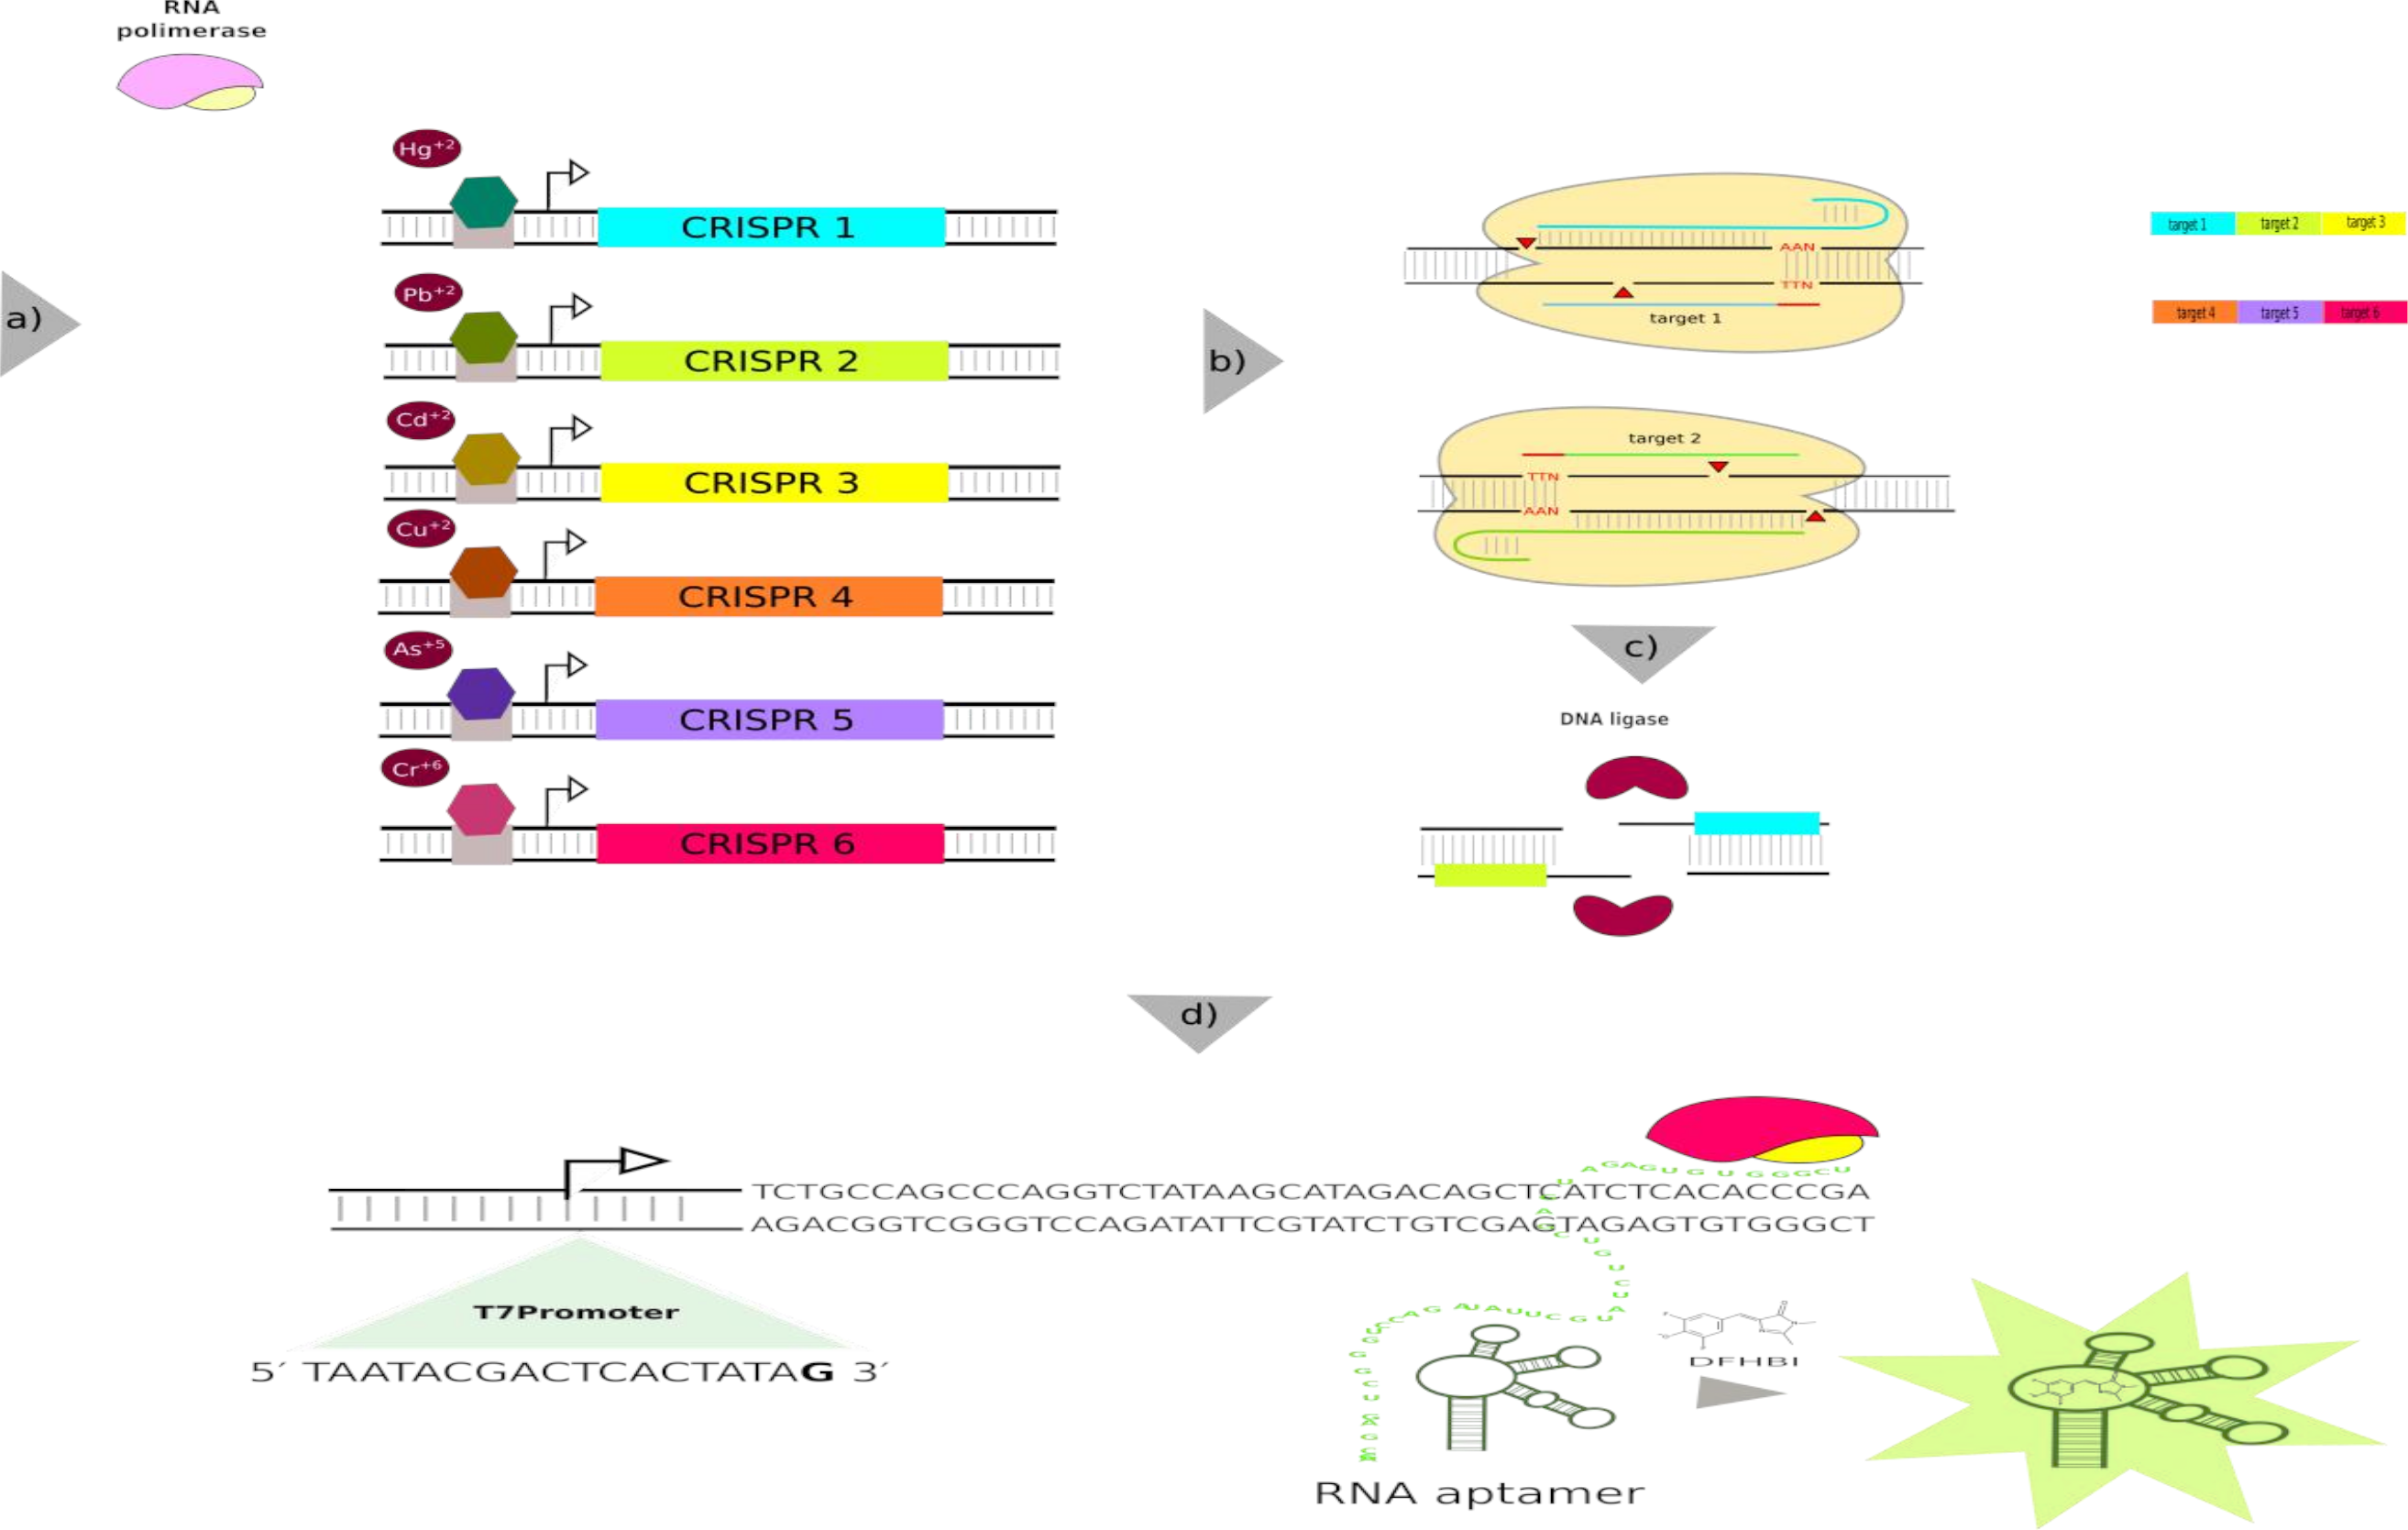
\includegraphics[width=1\textwidth]{discussion/chapter/figs/dnalogic.png}
  \caption{Proposed DNALogic system. A) crRNA expression is regulated by inducible promoters B) Ribonucleoprotein formation is followed by recognition and cutting of the target DNA C) Ligation of the overhangs produced by the Ribonucleoprotein generates a transcriptional unit D) Expression of the transcriptional unit generates a functional fluorescent RNA aptamer.}
  \label{fig.discu1}
\end{figure}

Even though here we use a population of living cells, these could be replaced by a totally in vitro reaction where a transcriptional-only genetic network can be used, without further need of translation. Each agent in this case, rather than a cell, can be a plasmid or a double stranded DNA that does not possess functional transcriptional networks. As cell-free systems can assemble DNA parts in vitro at very low cost by using cell extracts instead of enzyme cocktails \citep{casini2014one} and Golden Gate Assembly is an excellent tool to assemble multiple DNA fragments in a defined linear order, by using type IIS restriction enzymes \citep{engler2008one} , these techniques may be combined to generate a new and inexpensive in vitro system, which through DNA assembly and processing (hereafter DNALogic) would be able to sidestep common problems associated with the use of live cell based systems. As a "triggering" step is vital for the DNALogic processing machinery, the novel CRISPR/Cpf1 technology (or similar) could be used to generate the respective recognition and cutting steps. CRISPR/Cpf1 generates 5' overhanging cuts, producing 8 nt sticky ends and cleaving at the 14th base from the PAM site TTN \citep{Lei2017a, li2016c}. Due to its similarities to Type IIS restriction enzymes, Cpf1 or any simile enzyme can be used to generate a new kind of Golden Gate Assembly, which would not rely on the presence or absence of cutting sites, but on gRNA. The gRNA expression system can be combined with the recognition step, working as a transduction system between the detection and processing steps. This CRISPR triggered sequence recognition, followed by cutting and ligation steps, would result not only in a fully functional transcriptional unit, but also in a different double stranded genetic sequence, complying with the parameters for synthetic memory proposed and demonstrated in vivo by \citet{siuti2013synthetic}. This would create DNA memory that can not only be later amplified and processed by sequencing and/or PCR (late response), but also generating RNA expression of a fluorescent aptamer or a further gRNA if there would be formation of a proper transcriptional unit (immediate response). Proposed mechanisms can be seen on Figure \ref{fig.discu1}. 
RNA aptamers also suffer from several limitations as incorrect folding is observed under non optimal thermal or ionic conditions \citep{autour2016ispinach}. Even though improved aptamers with a stronger secondary structure, such as Broccoli and iSpinach, show increased stability under non-optimal conditions \citep{filonov2014broccoli, autour2016ispinach}, both aptamers are based in the 95 base core sequence of Spinach2 which need to be flanked by a tRNA scaffold, to increase the stability of their secondary structures \citep{filonov2014broccoli, autour2016ispinach, strack2013superfolding}. However, most of them were designed for in vivo usage (e.g. analysing RNA quantities) and have not been tested as outputs for a cell-free sensor besides this work and the one from \citet{jung2020cell}. Such a sensor could require only transcription, not translation, thus being faster and simpler.

Cell-free systems (CFS) are not without their limitations; since their very nature is to be a defined, precisely controlled system that lacks self-replicating functionality, they depend on a limited quantity of supplies, such as ATP, amino acids, and nucleotides \citep{kwon2015high}. Even though the coupling of transcription and translation accelerates the product formation, proteins still need to acquire their secondary, tertiary or even quaternary conformation to become functional, even sometimes needing post-translational modifications to work. 

Consequently, in-vitro synthesis of protein is limited by two dimensions: the overall maximum protein amount that can be synthesized with the supplied components, and the time during which the CFS stays active before background processes and chemical deterioration have used up supplies or inactivated the system \citep{carlson2012cell, bernhard2013cell,kwon2015high}. One of the most promising applications of CFS is the possibility of designing cell-free biosensors, which do not present a living prospect subject to the current GMO legal regulations and offer an alternative to standard analytical techniques, such as ICP-MS and ICP-OES. However, cell-free biosensors that rely on protein expression also present the common limitations of CFS, such as a long response time and a lack of precursor regeneration. Sensors that could function without the need for protein expression would drastically reduce the requirements for such a system.
\begin{figure}[!ht]
  \centering
  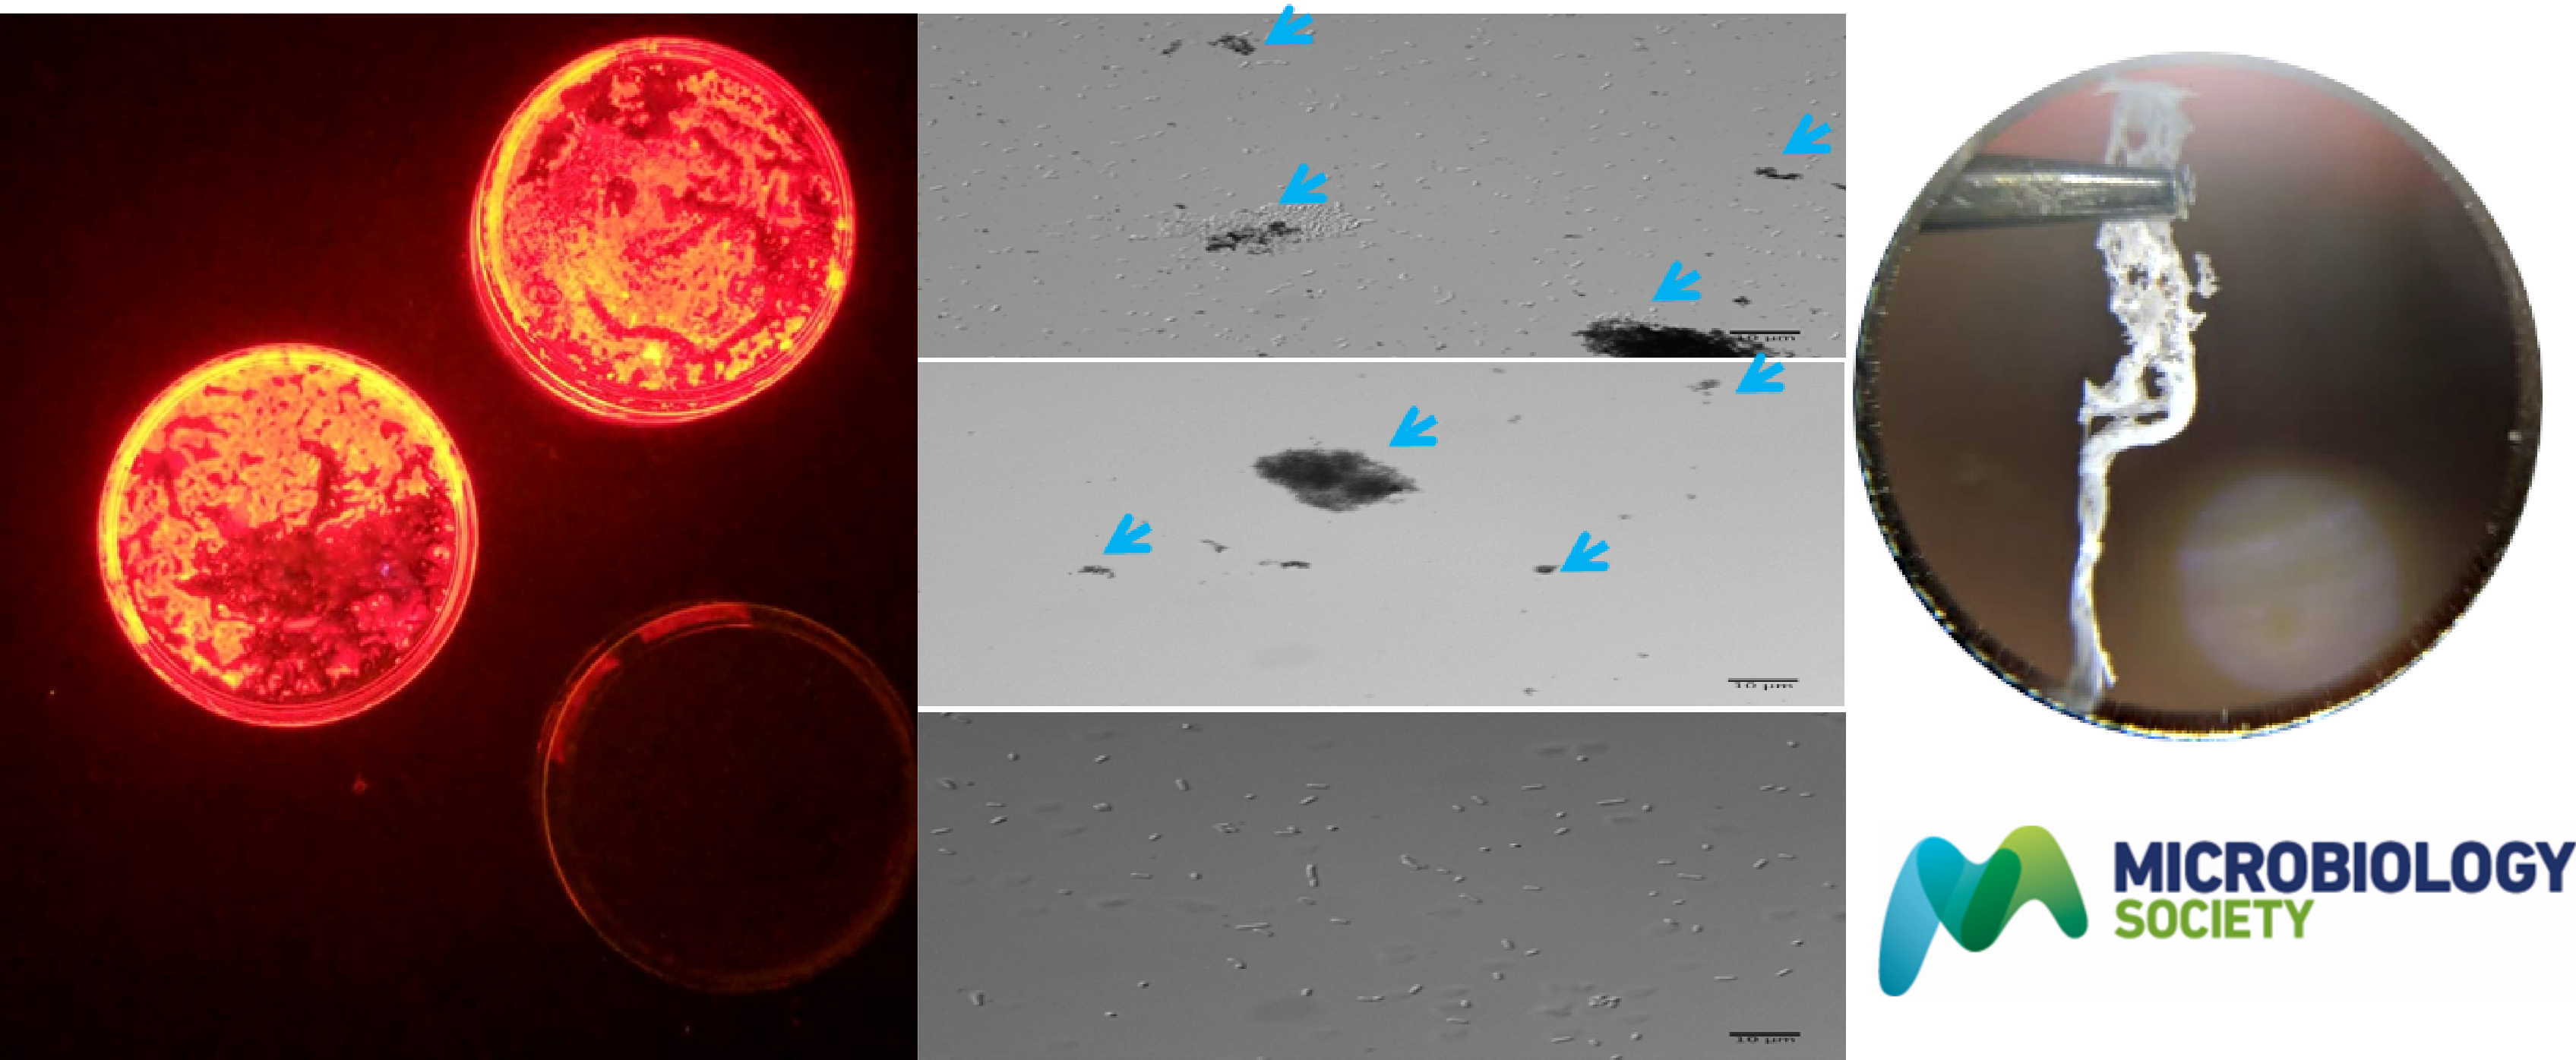
\includegraphics[width=0.9\textwidth]{discussion/chapter/figs/bioplastics.png}
  \caption{PHB Production Using Cell-Free Systems. Left. Bioplastic detection under blue light after Nile Red staining. Middle. in vivo and in vitro PHB production. Right. Bioplastic produced and purified from CH34 cultures. Work sponsored by the Microbiology Society and performed with the help of Nuoya Chen}
  \label{fig.discu2}
\end{figure}

\cite{moore2017cell} have attempted to solve this issue by using non-model bacteria, such as \textit{Bacillus} or \textit{Streptomyces}, for the generation of new cell-free TX/TL systems. This approach can be applied to other organisms, such as extremophiles, in order to use their unique capacities. For example, in this thesis is used the non-model bacteria \textit{Cupriavidus metallidurans} which possesses the capability to tolerate, remove and degrade diverse environmental pollutants \citep{millacura2017degradation}. This cell-free extract is simple to prepare by using a low-salt buffer and shows increased tolerance for heavy metals making it possibly superior to others as a heavy metal sensor. Preliminary results show that the anabolic and catabolic capabilities of this cell extract are conserved after lysis, here demonstrated via bioplastic production (Figure \ref{fig.discu2})  and by catechol degradation via catechol-1,2-dyoxygenases and catechol-2,3-dyoxygenases (Figure \ref{fig.discu3}) respectively. Even though further development is required, this novel cell-free chassis could become a standard for mass production considering versatility and robustness showed once compared with \textit{E. coli} based ones.

\begin{figure}[!ht]
  \centering
  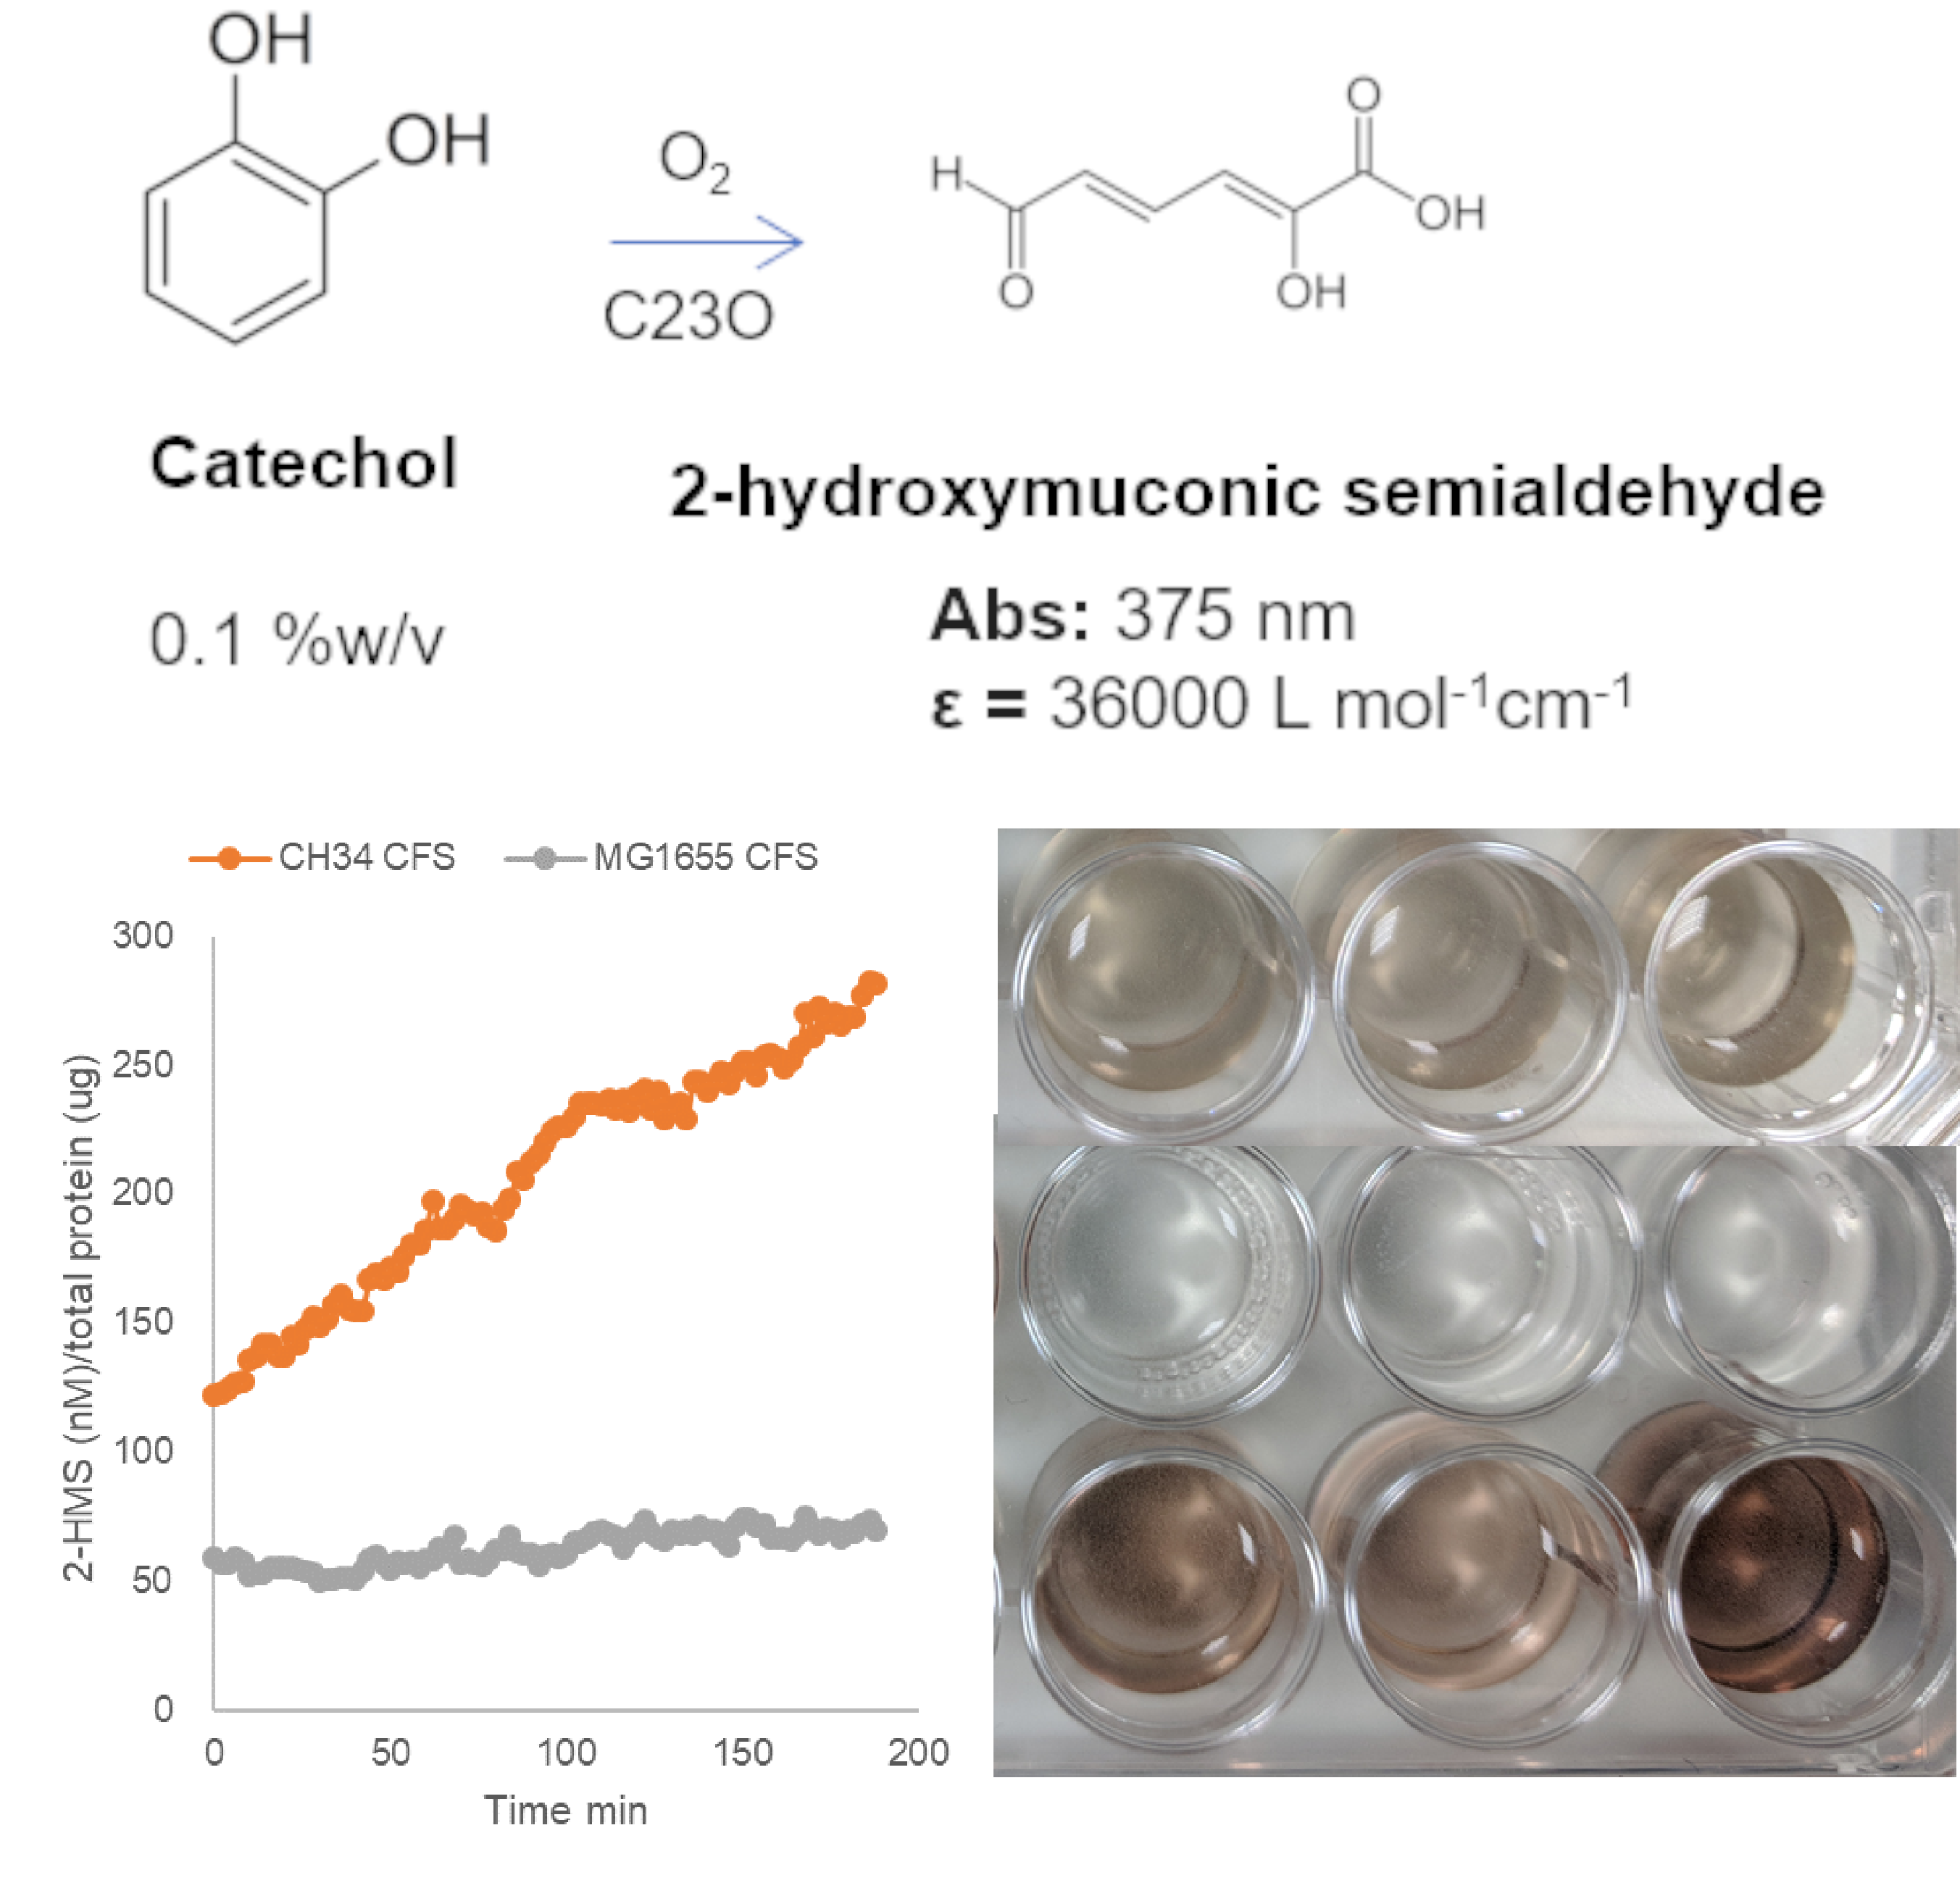
\includegraphics[width=0.7\textwidth]{discussion/chapter/figs/degradation.png}
  \caption{Catechol-2,3-dioxygenase activity assay using \textit{Cupriavidus} cell-free system. Upper. beta-cleavage of the catechol ring and formation of 2-hydroxymuconic semialdehyde. Bottom. \textit{Cupriavidus} cell-free catechol degradation.}
  \label{fig.discu3}
\end{figure}


Another challenge for CFS is to analyse multiple variables simultaneously. As they rely on the normal cell processing/synthesis machinery (interaction between transcription factors, polymerases, ribosomes, and other diverse macromolecules), they suffer the same issues as a living organism. Furthermore, when complex interactions are carried out, problems may arise due to kinetic mismatches, lack of oscillation or Boolean/Reversible designs \citep{guz2016bioelectronic}. The generation of cell-free systems that respond to variables using totally synthetic processing machinery seems to be one of the most promising approaches. There have been some attempts to generate logic gates without mimicking normal cell machinery \citep{bordoy2016transcriptional, chatterjee2016computing, kim2011switch, zhang2016dna}, however, due to their dependence on translation and/or the need for manual addition of foreign oligonucleotides (Kim et al., 2014) they still show slow response. Additionally, some of them rely on recombination processes that make their implementation even more complicated than under \textit{in vivo} conditions \citep{zhang2016dna}. In electronics, a single circuit accepts one or more binary inputs to generate one or more binary outputs. There have been many attempts to replicate such circuits using in vivo genetic networks. A typical biological logic gate consists of an output macromolecule that is produced only if the corresponding pattern of inputs is present, inputs that are commonly associated with the presence of transcriptional regulators, transcription factors, polymerases or other macromolecules \citep{silva2008mining}.


Since scientific data in Synthetic Biology is massively increasing, novel analysis techniques than go further than standard human gathering need to be implemented. For instance, machine learning algorithms and artificial intelligence can be used to gather, process, and analyse scientific reports. An example is shown in Figure \ref{fig.discu4} were Natural Language Processing techniques were used to analyse the complete collection on Synthetic Biology publicly available on BioRxiv. There are hundreds of scientific research manuscripts published every year and information can get missing or hidden-in-plain-sight. Machine learning could grant the link between the words used in research articles and the data referenced on it, also it could allow prediction of new technologies to come by simply analysing both topics of high and low interest for the research community. With enough computational power massive quantities of data could be analysed even in real-time, crossing not only with official repositories but also social networks specialised in research or not.

\begin{figure}[!ht]
  \centering
  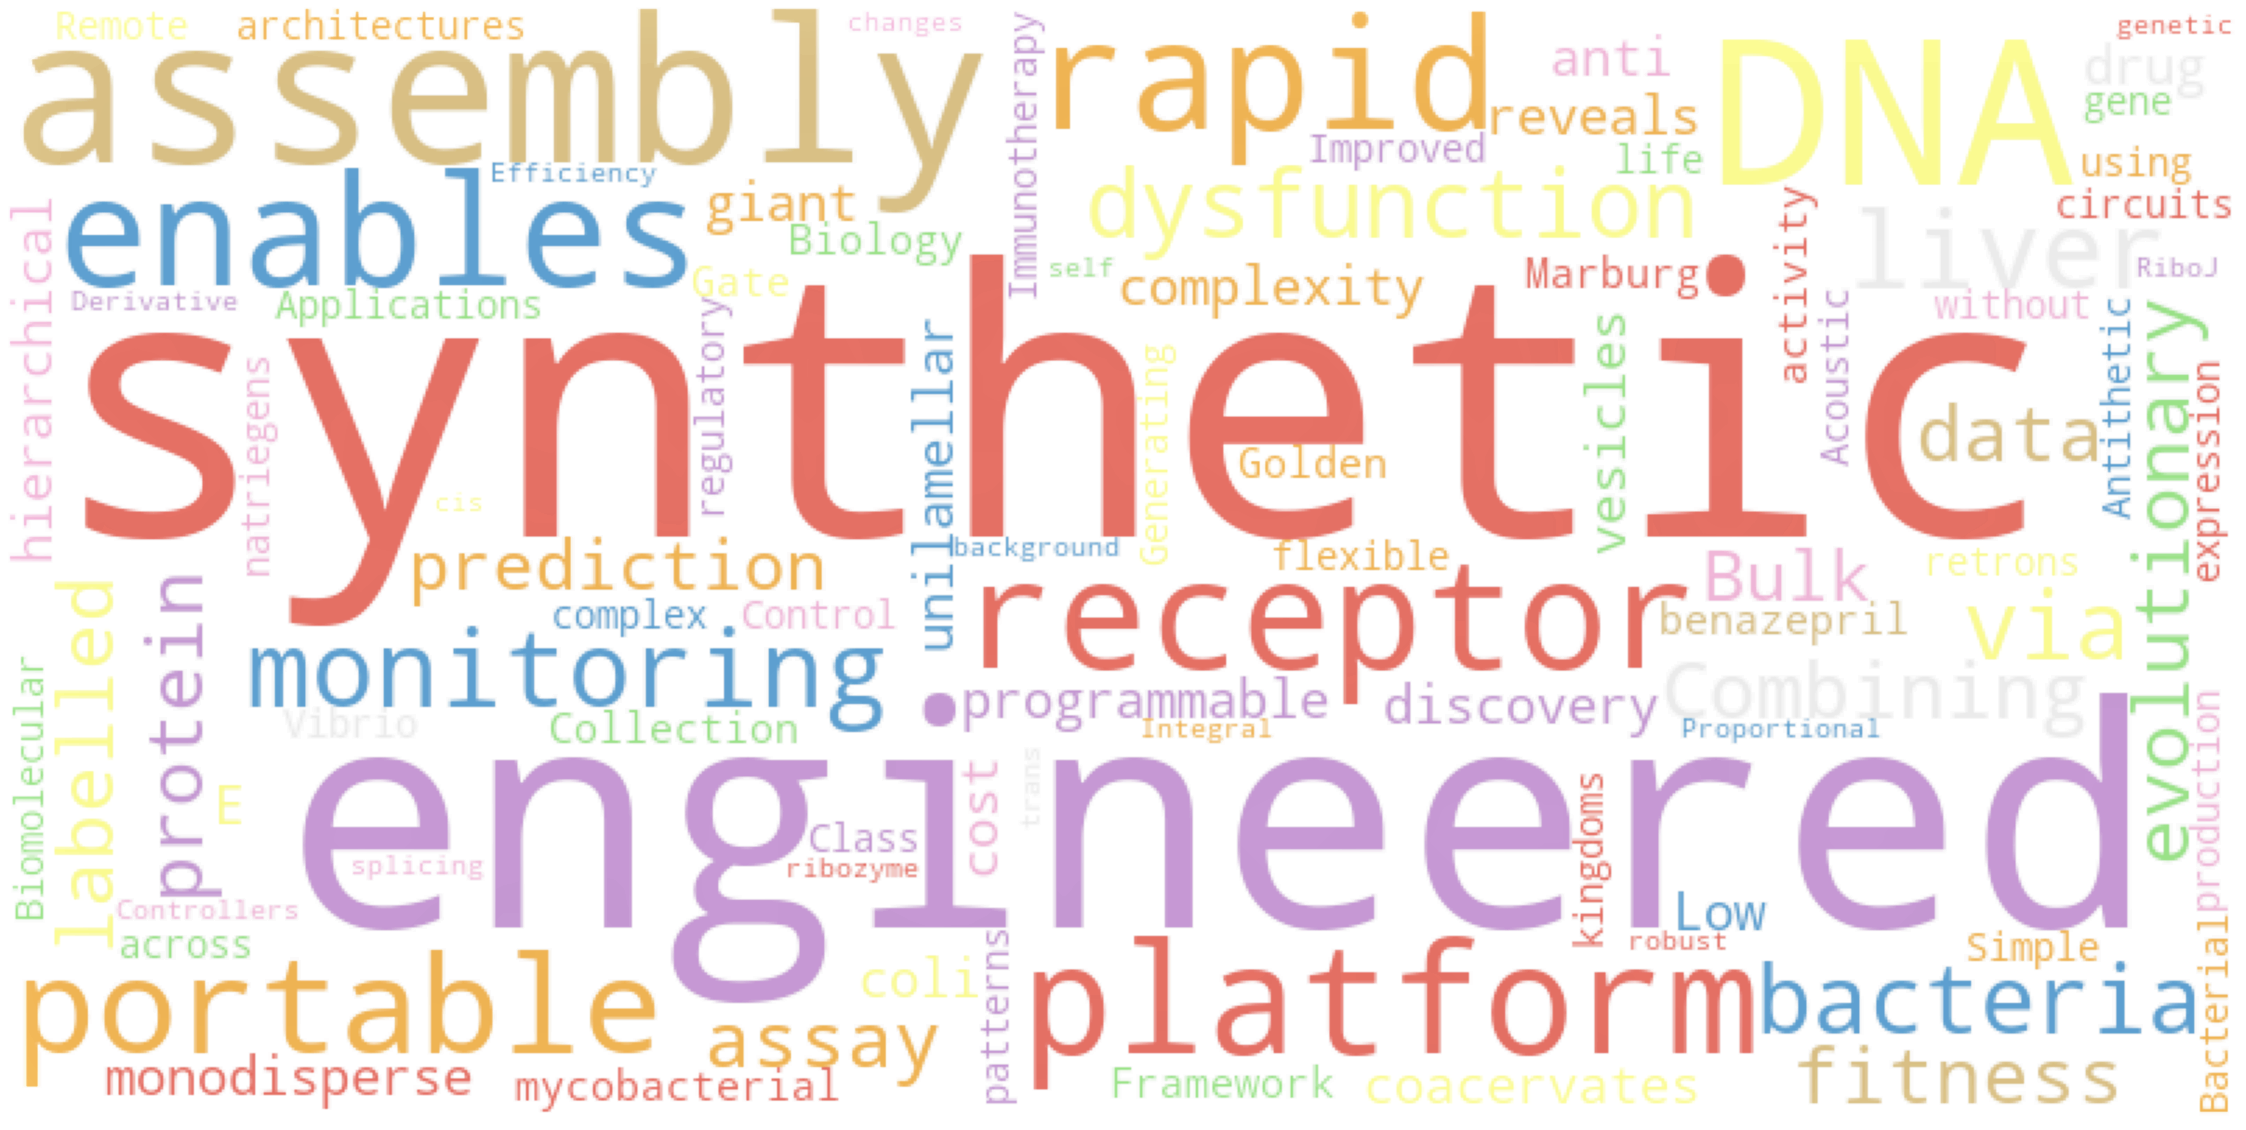
\includegraphics[width=0.9\textwidth]{discussion/chapter/figs/wordcloud.png}
  \caption{Natural Language Processing (NLP) analysis of BioRxiv's Synthetic Biology collection. Article titles from the entire BioRxiv synthetic biology collection were analysed using Natural Language processing (NLP) techniques. All 220 articles were collected via web scrapping and unnested into 2552 tokens and stopwords later removed. Most common 100 words are here plotted as a WordCloud. Full analysis available at https://gist.github.com/millacurafa/0151170cf971d1ae46092f32b4d7c2a2}
  \label{fig.discu4}
\end{figure}

Another interesting feature of current technologies would be the usage of machine and deep learning algorithms to analyse metagenomic or genomic analyses. Sequencing techniques are getting cheaper each time and since it has been proved than mutations can be generated during genetical engineering, rather than just analysing a few genes and phenotypes the scientific community could start preparing into massive genomic analyses. Assemblies could be simplified, together with SNPs and INDELs detection. Additionally, algorithms could be generated to generate inexistent sequences that would allow to go even further than what it is available in nature. For instance, the terms minimal absent words (MAWs), nullomers and primes all describe sequences that do not occur in the entire genome or proteome of an organism \citep{hampikian2007absent, koulouras2020significant}. Primes are the shortest sequences that are not found across all known species, whereas nullomers are the shortest possible absent motifs in a species, MAWs including both definitions. But what are the shortest or even largest sequences present in all organisms (aka popularly as the sequence of god). These still have theoretical significance as sequences that cannot exist on nature due to them causing death in organisms or simply because during natural selection were not prioritized. A world of new opportunities lay in sequences that are beyond nature and the scope of Synthetic Biology should be broaden in that direction allowing to solve the unsolvable.

%========================= Appendix ========================= 
\renewcommand{\chaptermark}[1]{%
 \markboth{\MakeUppercase{%
 \appendixname} \ \thechapter.%
 \ #1}{}}
%\renewcommand{\dir}{../appendix/appendix}
%\input{\dir/appendix.tex}

%========================= BIBLIOGRAPHY ========================= 
\ifthenelse{\boolean{edthesis}}
 {
 \begin{singlespace}
}
{
  \backmatter
}
\def\bibname{References}
\addcontentsline{toc}{chapter}{References}
\bibliography{bibliography}
\ifthenelse{\boolean{edthesis}}
 {
  \end{singlespace}
 }{}

